\documentclass[11pt]{article}
\usepackage[utf8]{inputenc}
\usepackage{amsmath,amssymb,amsfonts}
\usepackage{graphicx}
\usepackage{xcolor}
\usepackage{booktabs}
\usepackage{siunitx}
\usepackage{hyperref}
\usepackage{subcaption}
\usepackage{geometry}
\usepackage{placeins}
\geometry{margin=2.5cm}
\usepackage{changepage}
\usepackage{ulem}

\newcommand{\E}{\mathbb{E}}
\newcommand{\Var}{\mathrm{Var}}
\usepackage{authblk}

\title{Do proprietary and client metaorders impact prices \\ in a different way?}
%Metaorders, Price Impact, and Crowding:\\Evidence from Proprietary and Client Flow}
\author[1]{Daniele Maria Di Nosse\textsuperscript{\dag}}
\author[2]{Francesco Gigante}
\author[1]{Fabrizio Lillo}
\author[2]{Antonio Russo}

\affil[1]{Scuola Normale Superiore, Pisa, Italy}
\affil[2]{Consob, Rome, Italy}
\date{\today}

\begin{document}

\maketitle
\begin{center}
  \footnotesize
  \dag Corresponding author. Email: \texttt{daniele.dinosse@sns.it}
\end{center}

\begin{abstract}
Large trading decisions are typically split into many smaller trades and executed through market members, 
either for the member’s own account or on behalf of clients. This paper asks whether these two trading 
capacities generate the same market footprint. Using trade-by-trade data for FTSE MIB constituents from June 
2024 to May 2025, with aggressive trades attributed to members and labelled as proprietary or client flow, we 
reconstruct member-level metaorders and compare their execution characteristics, price impact, impact dynamics, 
and crowding environment.
Proprietary and client metaorders are similar in their broad statistical properties: both display heterogeneous, 
heavy-tailed distributions of size, duration, and relative volume. The main execution-level difference is that 
proprietary metaorders tend to trade with higher participation rates. The price response, however, differs more 
sharply. Client metaorders produce an impact curve close to the square-root law and their impact partly reverts 
after execution. Proprietary metaorders display a more concave impact law, higher fitted impact over most of the 
observed size range, and a more persistent post-execution footprint.
Crowding reveals the mechanism only in part. Client flow is more strongly aligned with same-day client imbalance, 
especially at high participation rates, so daily crowding is not by itself the source of the proprietary impact 
premium. The relevant distinction appears at the execution-time scale: proprietary metaorders are more often 
surrounded by overlapping flow in the same direction. Controlling for this active directional overlap weakens 
the proprietary premium. Overall, the evidence shows that proprietary and client metaorders should not be pooled: 
trading capacity matters for impact, persistence, and the interpretation of crowded order flow.
\end{abstract}

\section{Introduction}
% {\bf In financial markets, such as the one investigated here, the access to the trading is provided via market members who can trade either on behalf of their client or as proprietary trading.... 
% As the goal of this project is to study the differences and the interplay 
% between proprietary and client metaorders....}

Understanding how large orders move prices is central both to execution-cost analysis and to theories
of price formation. In modern electronic markets, however, large trading decisions typically reach
the market through intermediating members, who may execute on behalf of clients or trade for
their own account. This distinction is economically meaningful: proprietary and client trades may
differ in information content, execution style, inventory motives, and exposure to crowding, with
potentially different consequences for both the level and the persistence of market impact. Related
evidence that order-flow categories should not be pooled is provided by
\cite{ChakrabartyCoxUpson2024RetailOrderFlow}, who show that off-exchange retail,
off-exchange institutional, and on-exchange order flow differ substantially in their
volume-adjusted contribution to price discovery. Our distinction is different: client flow in our
data should not be interpreted as retail flow, since it includes orders executed on behalf of
end-clients that may themselves be institutional investors. Yet most empirical studies of
metaorders do not cleanly separate proprietary and client trading capacities. Using trade-by-trade
data for FTSE MIB constituents in which aggressive trades are attributed to individual members
and labelled as proprietary or client, this paper exploits that separation to compare the properties,
price impact, and crowding of proprietary and client metaorders within a common empirical
framework.


A robust empirical regularity in market microstructure is the
non-linear, concave relation between the average price impact of large
orders and their size, measured either in volume or in execution time. When a metaorder of total size $Q$ shares is executed
over a day by slicing it into many smaller trades, the average price
change $\Delta p$ typically scales as a power law,
\begin{equation}
  \Delta p =Y \epsilon \sigma_D \left(\frac{Q}{V_D}\right)^\gamma, \qquad 0 < \gamma < 1,
\end{equation}
where $\epsilon=\pm  1$ is the sign of the trade, $\sigma_D$ is the daily volatility and $V_D$ the daily volume. 
Here, $\Delta p = p_{\mathrm{end}_j}-p_{\mathrm{start}_j}$ is the peak impact of the metaorder started at price $p_{\mathrm{start}_j}$ and ended at price $p_{\mathrm{end}_j}$. 
The constant $Y$ captures the execution quality and might depend, for example, on the trading algorithm. The ``square-root law'' arises when $\gamma \approx 1/2$ and it has been observed across markets and asset classes .
This behavior has been documented in a wide range of institutional
datasets and synthetic metaorder reconstructions, and is remarkably
robust to variations in the microstructure, i.e. tick size, asset type, etc \cite{BacryEtAl2014, Torre1997, AlmgrenEtAl2005, EngleEtAl2008, MastromatteoEtAl2014, BrokmannEtAl2014, SatoKanazawa2024}.

At the same time, institutional trading activity is highly crowded \cite{PuckettYan2008,Sias2004,DasguptaPratVerardo2011}:
different investors often trade in the same direction on the same names
and days, which amplifies execution costs through co-impact.
In co-impact models, the aggregate price response is driven by the joint
distribution of metaorder signs and sizes, with correlations in order
flow leading to a non-linear impact surface and to important differences
between idiosyncratic and crowded trades \cite{BucciEtAl2020, BriereEtAl2019}. 

% {\bf Altre referenze \textcolor{blue}{Ho aggiunto \cite{PuckettYan2008,Sias2004,DasguptaPratVerardo2011} e \cite{BriereEtAl2019}}}.

The present analysis focuses on a high-frequency dataset where
trade-by-trade aggressive activity can be attributed to individual
members and separated into proprietary and client flows. Using these data, we 
reconstruct metaorders as same-sign sequences of aggressive trades at the member level and
document the empirical distribution of their durations, sizes, relative sizes in units of daily volume, and execution
participation rates. We then estimate a volatility-normalised power-law impact function as a function of the metaorder's 
size, and study crowding measures for proprietary and client flows.

Against this background, we investigate the following questions:

\begin{enumerate}
    \item Do proprietary and client metaorders differ systematically in their basic execution characteristics, such as size, duration, participation rate, and distribution across members?
    \item Do proprietary and client metaorders obey the same impact law, or do they differ in the scale and concavity of price impact once size and impact are properly normalised?
    \item Do their dynamic impact profiles differ, in particular in the build-up of impact during execution and in the decay or persistence after completion?
    \item How does crowding differ across proprietary and client flow, both within each group and in their cross-group interaction? Does crowding help explain the observed differences in impact between proprietary and client metaorders?
\end{enumerate}

% {\bf Possible research questions:

% \begin{itemize}
% \item Are the metaorders executed on behalf of clients or on a proprietary basis statistically different in their static properties?

% \item Is the market impact (trajectory, peak, decay) of metaorders executed on behalf of clients or on a proprietary basis statistically different? Perform the comparison both for the pooled samples across members and for client and proprietary within each member 

% \item What are the possible reasons for different properties?
% Reasons of possible differences:
% \begin{itemize}
% \item Degree of information
% \item Front running
% \item Execution styles
% \item .......
% \end{itemize}
% \item Is it possible that the difference of crowding characteristics of client and proprietary metaorder explains the different impact? The group crowding more should have larger impact.
% \end{itemize}
% }

We find that proprietary and client metaorders are similar in their broad distributional properties, but differ 
in execution aggressiveness and price response. Proprietary metaorders trade at higher participation rates, 
generate a more concave impact curve that lies above the client curve over most of the observed relative-size 
range, and retain a larger fraction of their impact after execution. Crowding measures help interpret this difference: 
even if client flow is more crowded at daily level, the proprietary impact premium 
is most weakened when controlling for directional active overlap during execution. Overall, the evidence shows that 
proprietary and client metaorders should not be pooled when possible: trading capacity matters for impact, persistence, 
and the interpretation of crowded order flow.

The remainder of the paper is organized as follows. Section~\ref{sec:data_metaorders} describes the trade-level data and the metaorder reconstruction procedure. Section~\ref{sec:descriptive_properties} documents the descriptive properties of proprietary and client metaorders, including their distributional features and execution schedules. Section~\ref{sec:impact_model} estimates and compares their price-impact laws and dynamic impact paths. Section~\ref{sec:crowding} studies aggregate, cross-group, participation-conditioned, and execution-time crowding, and evaluates whether these mechanisms explain the proprietary--client impact differences. Section~\ref{sec:member_prop_client_alignment} then studies the related but distinct question of member-level alignment between proprietary trading and same-member client flow. Section~\ref{sec:conclusion} concludes, while Appendix~\ref{app:member_nationality_results} collects member-nationality diagnostics and Italian-member robustness checks.

\section{Data and Metaorder Reconstruction}
\label{sec:data_metaorders}

This section describes the underlying trade-level dataset and the procedure used to reconstruct member-level metaorders.
We also define the per-metaorder quantities used throughout the descriptive analysis, impact estimation, and crowding results.

\subsection{Trade-level data}

We investigate an event-level sequence of aggressive trades for all the FTSE MIB constituents traded at Borsa Italiana
between June 6, 2024 and May 30, 2025, for a total of 251 trading days. The number of investigated stocks is 41.

For each trade $j$ we have an instrument identifier (ISIN) $k_j$, a timestamp $t_j$, an aggressive
direction $\varepsilon_j \in \{+1,-1\}$, with $\varepsilon_j = +1$ for aggressive buys and $\varepsilon_j=-1$ 
for aggressive sells, a traded volume $q_j > 0$ (number of shares), the first and last execution 
prices $p_{\mathrm{start}_j}, p_{\mathrm{end}_j}$, an aggressive capacity flag distinguishing proprietary 
(``dealing on own account'') from client (non-proprietary) trading, a client identifier and a member identifier. 

% \begin{itemize}
%   \item an instrument identifier (ISIN) $k_j$;
%   \item a timestamp $t_j$;
%   \item an aggressive direction $\varepsilon_j \in \{+1,-1\}$, with
%         $\varepsilon_j = +1$ for aggressive buys and $\varepsilon_j=-1$
%         for aggressive sells;
%   \item a traded volume $q_j > 0$ (number of shares);
%   \item the first and last execution prices $p_{\mathrm{start}_j}, p_{\mathrm{end}_j}$;
%   \item an aggressive capacity flag distinguishing proprietary (``dealing
%         on own account'') from client (non-proprietary) trading;
%   \item a client identifier and a member identifier.
% \end{itemize}

\begin{figure}[htbp]
    \centering
    \begin{subfigure}[b]{0.45\linewidth}
        \centering
        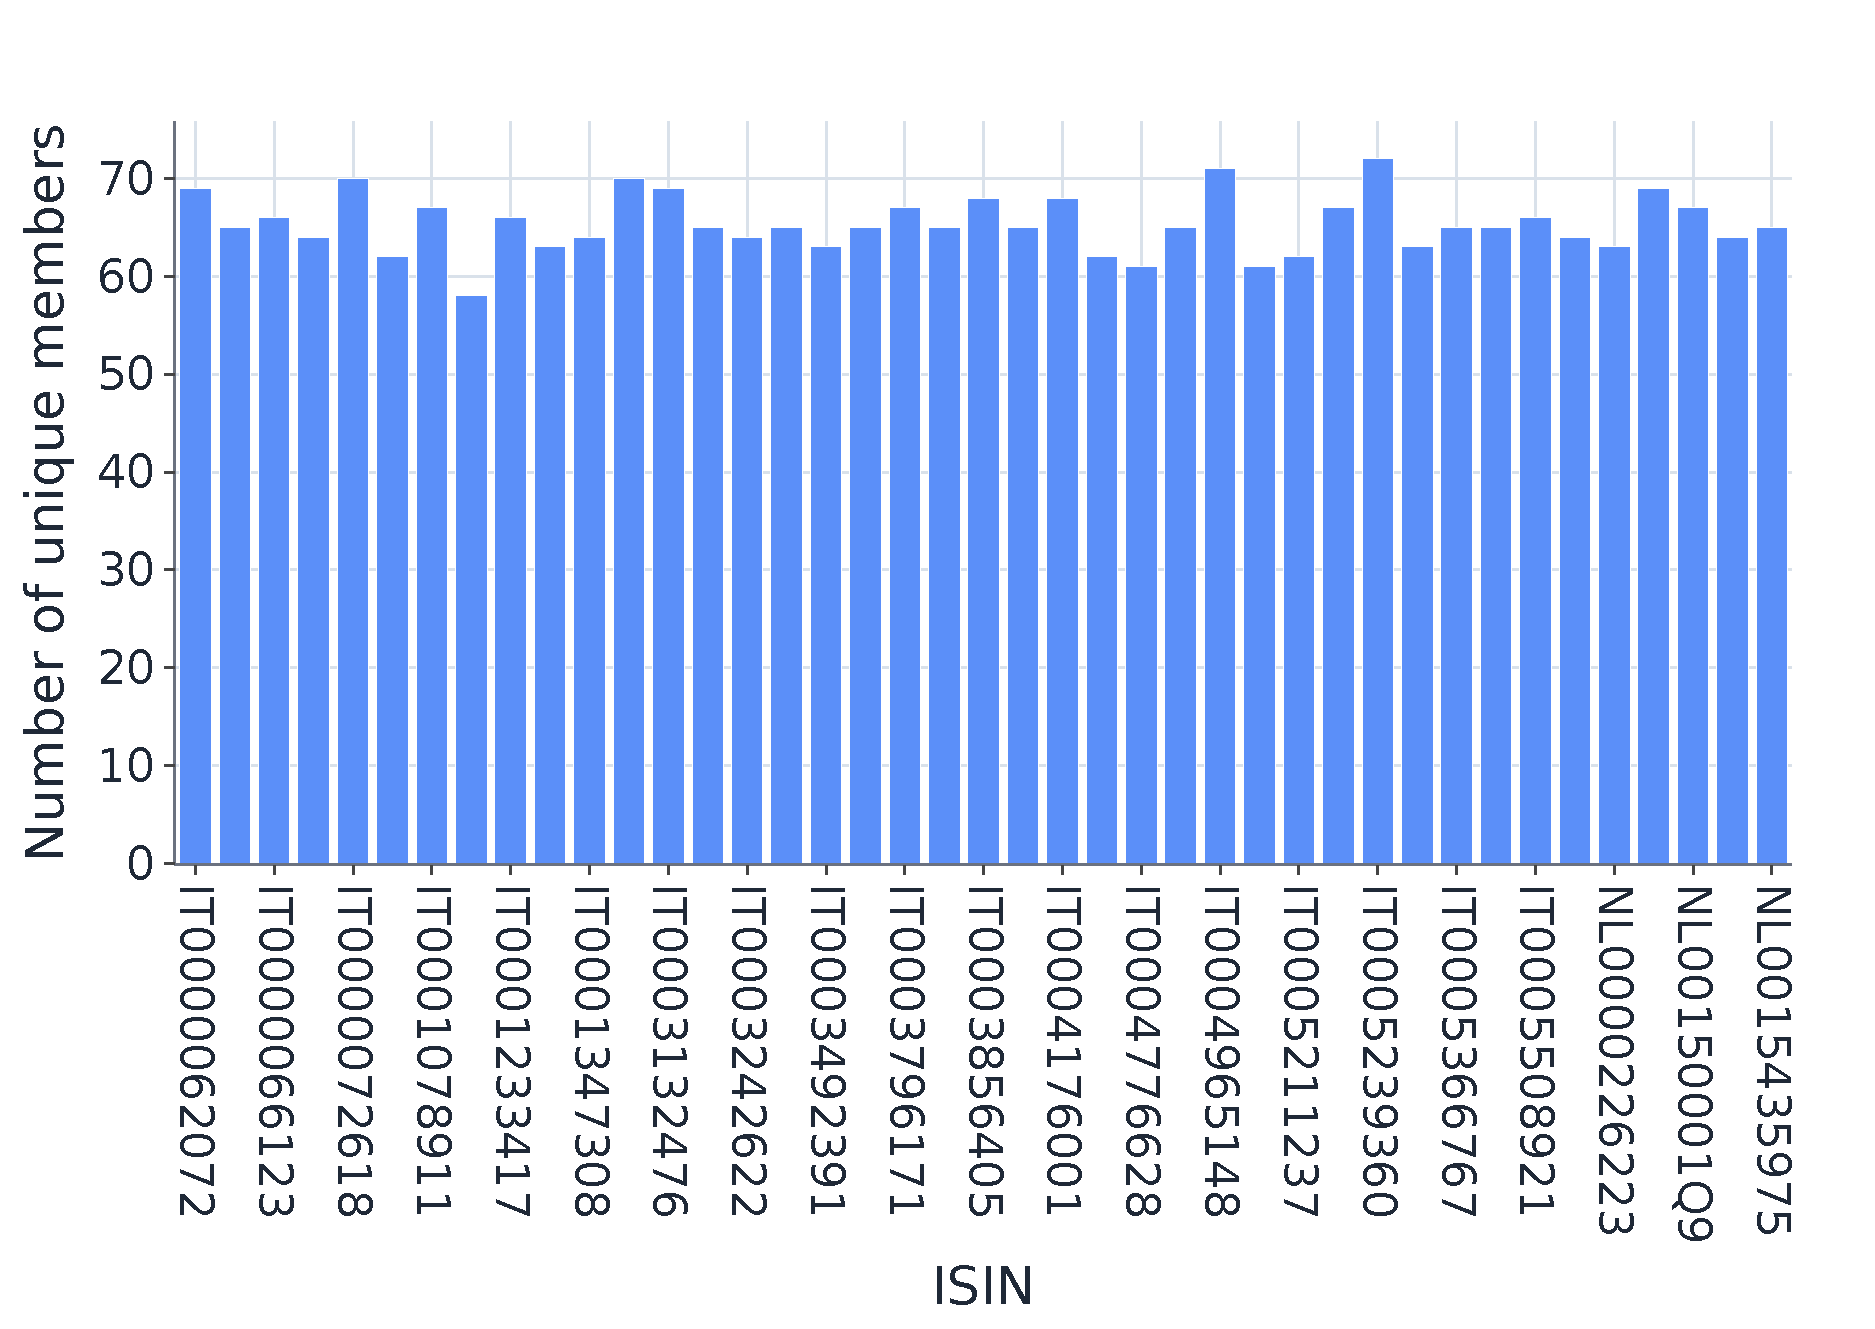
\includegraphics[width=\linewidth]{images/member_statistics/png/members_per_isin}
        \caption{Active members per ISIN.}
        \label{fig:members_isins}
    \end{subfigure}
%    \hfill
    \begin{subfigure}[b]{0.45\linewidth}
        \centering
        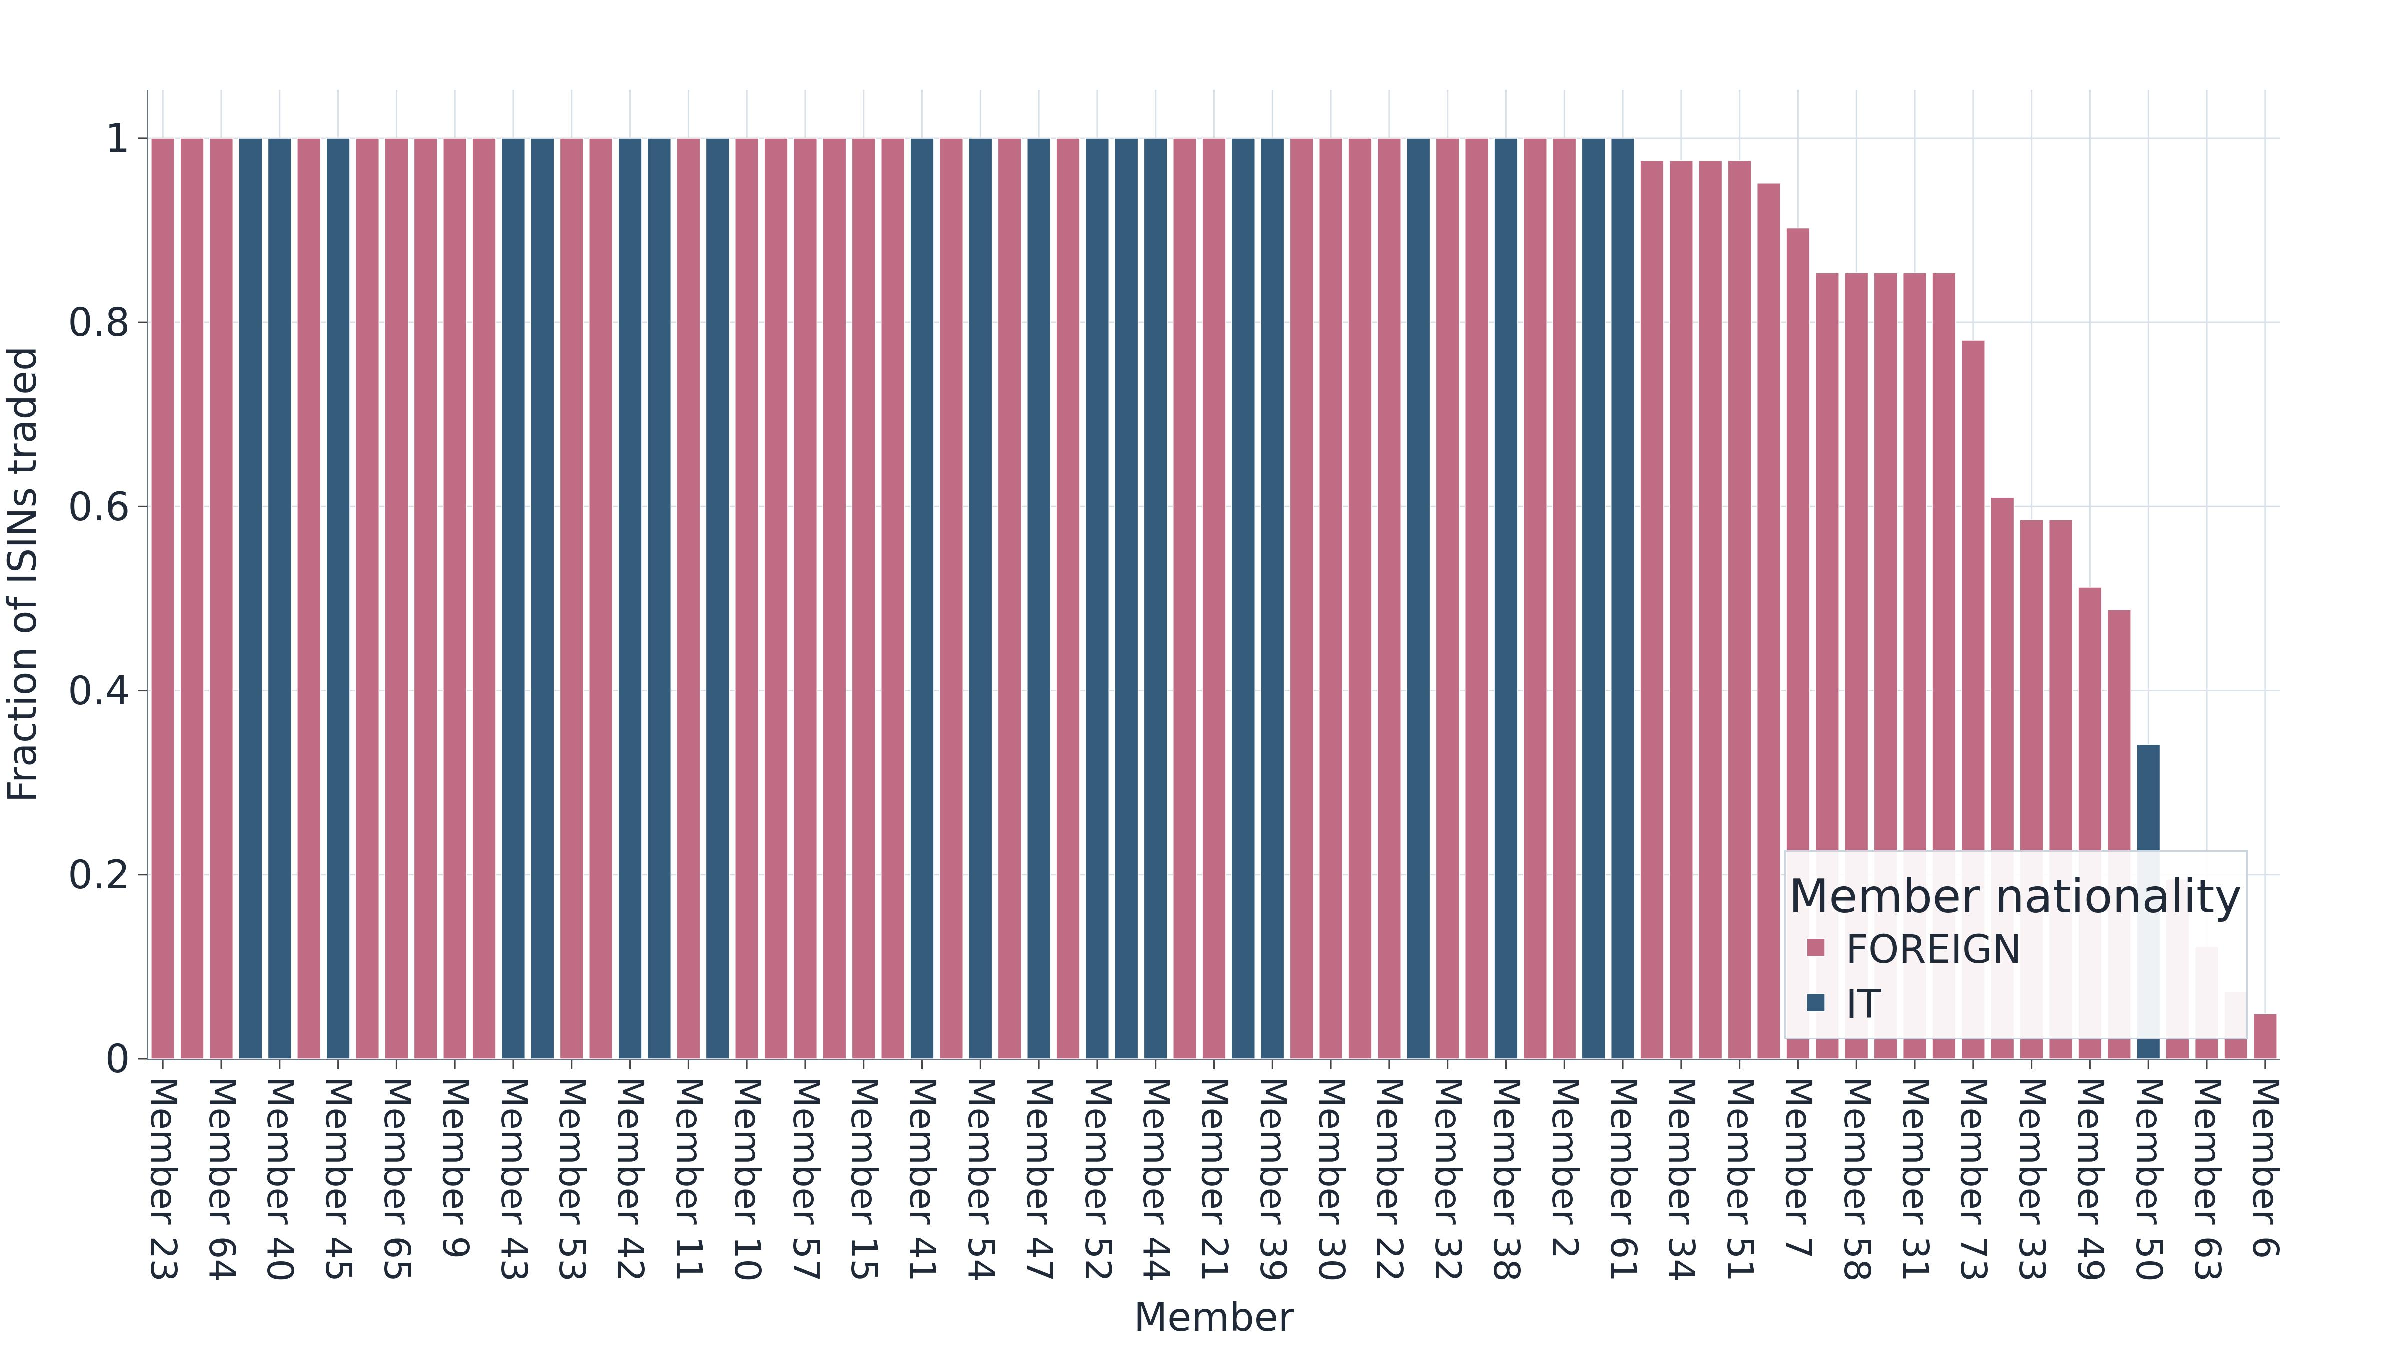
\includegraphics[width=\linewidth]{images/member_statistics/png/member_isin_coverage_per_member}
        \caption{ISIN coverage per member.}
        \label{fig:trades_per_member}
    \end{subfigure}
    % \caption{Analysis of member activity and market coverage across ISINs.}
    \caption{}
    \label{fig:member_statistics_combined}
\end{figure}

Only trades in the continuous trading session are used (from 09{:}30 to 17{:}30) and trades are sorted by time within 
each ISIN to form a time-ordered event stream. As the goal of this project is to study the differences and the interplay 
between proprietary and client metaorders, it is useful to collect some descriptive statistics about these two kinds of 
trades and the overall behavior of the market members. There are $73$ active members across all ISINs in the sample, 
and Figure~\ref{fig:members_isins} shows the number of active members per ISIN. The figures indicate that almost all 
members are active in almost all ISINs and that the majority of them traded all the assets, with a very small fraction 
focused on a smaller subset of the ISINs.

Across ISINs, the ratio between proprietary and client aggressive trades is relatively stable, as shown in 
Figure~\ref{fig:trades_per_isins}. Proprietary aggressive trades are consistently more numerous than client trades, 
with a ratio ranging from 0.60 to 1.30.

\begin{figure}[t]
    \centering
    \begin{subfigure}[b]{0.45\linewidth}
        \centering
        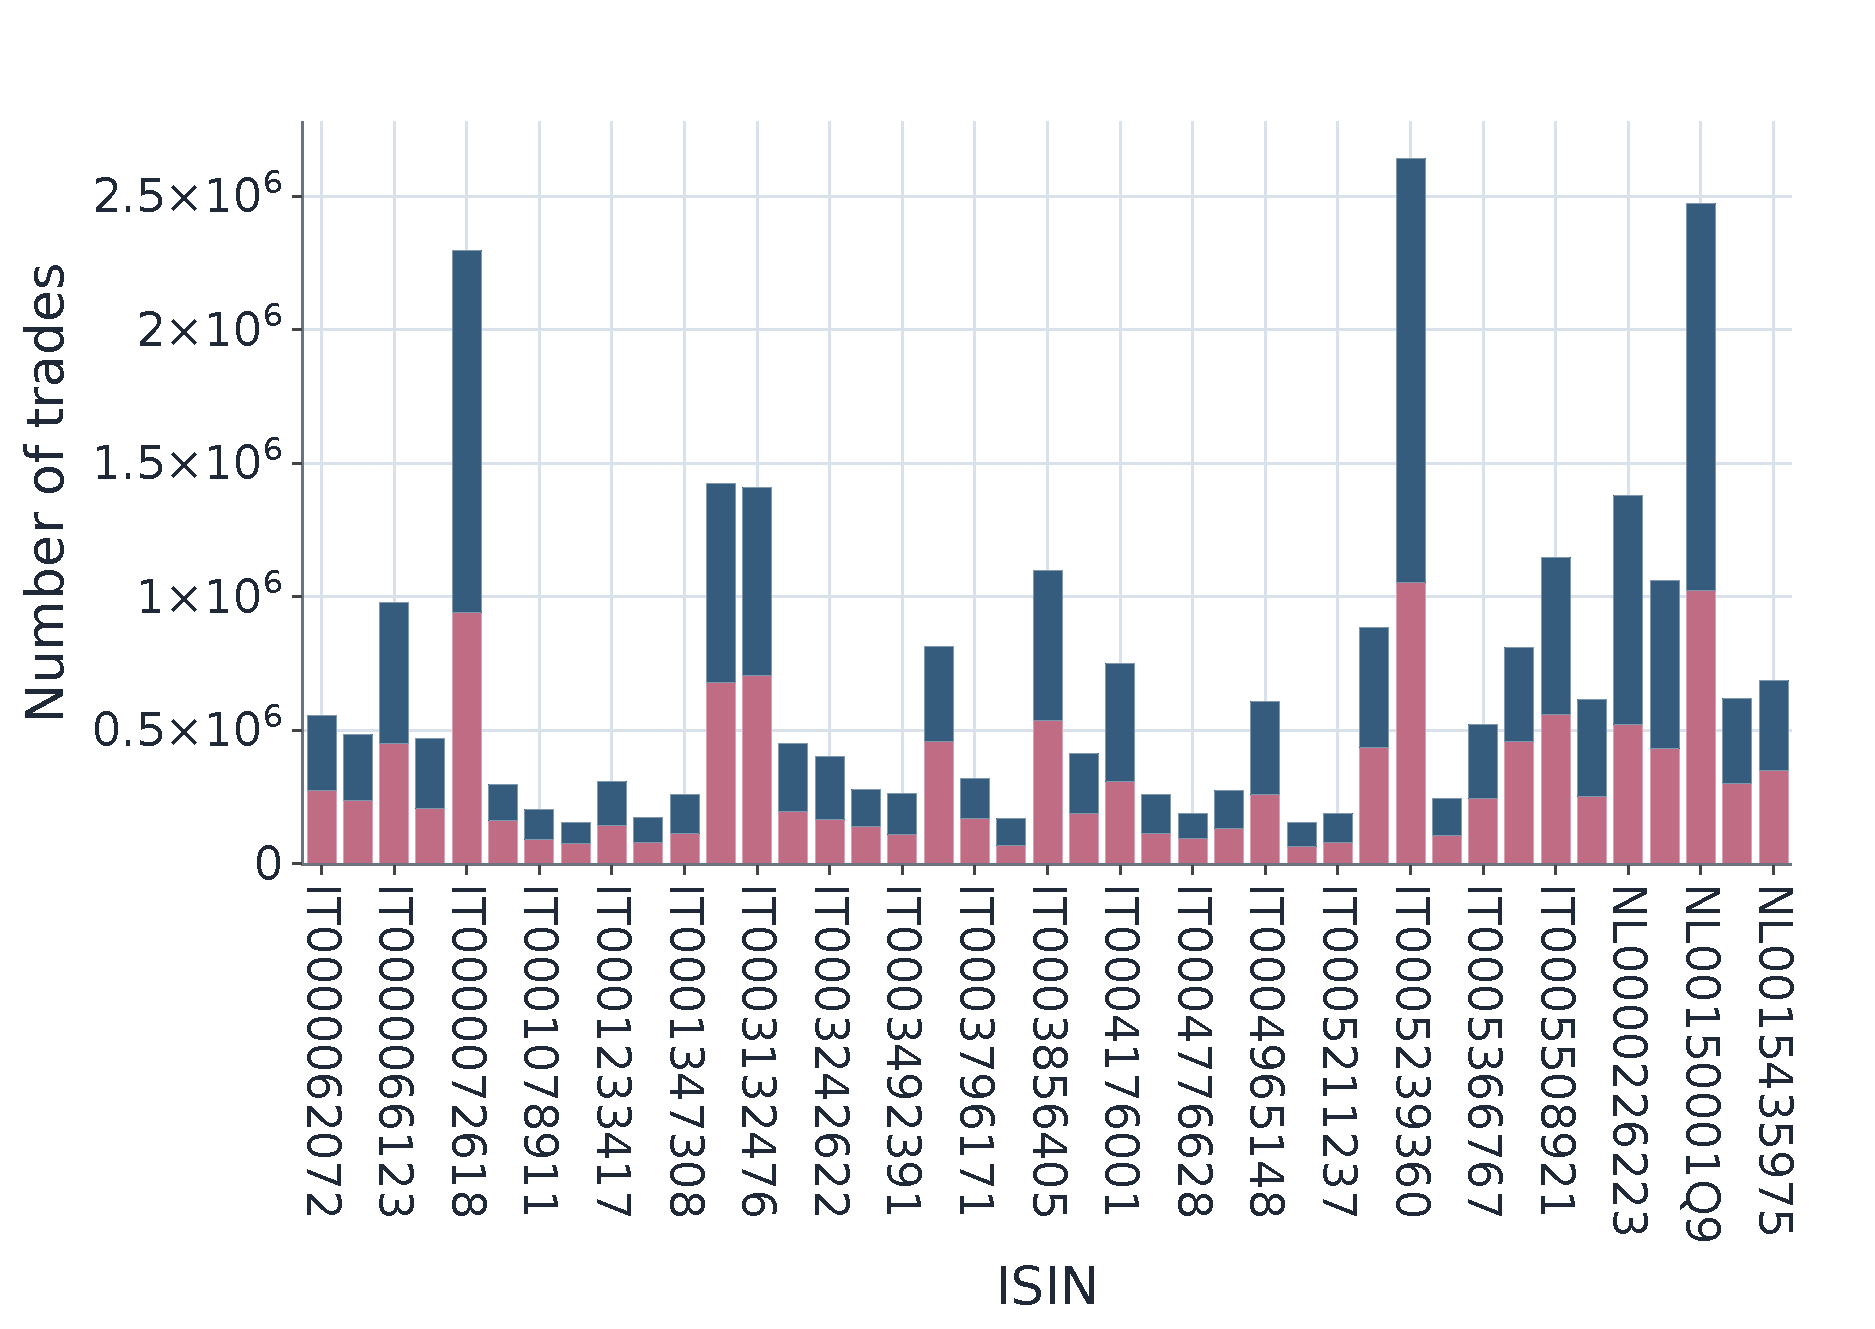
\includegraphics[width=\linewidth]{images/member_statistics/png/proprietary_vs_client_trades_per_isin}
        \caption{Number of proprietary and client trades per ISIN (blue: proprietary, red: client).}
        \label{fig:trades_per_isins}
    \end{subfigure}
%    \hfill
    \begin{subfigure}[b]{0.45\linewidth}
        \centering
        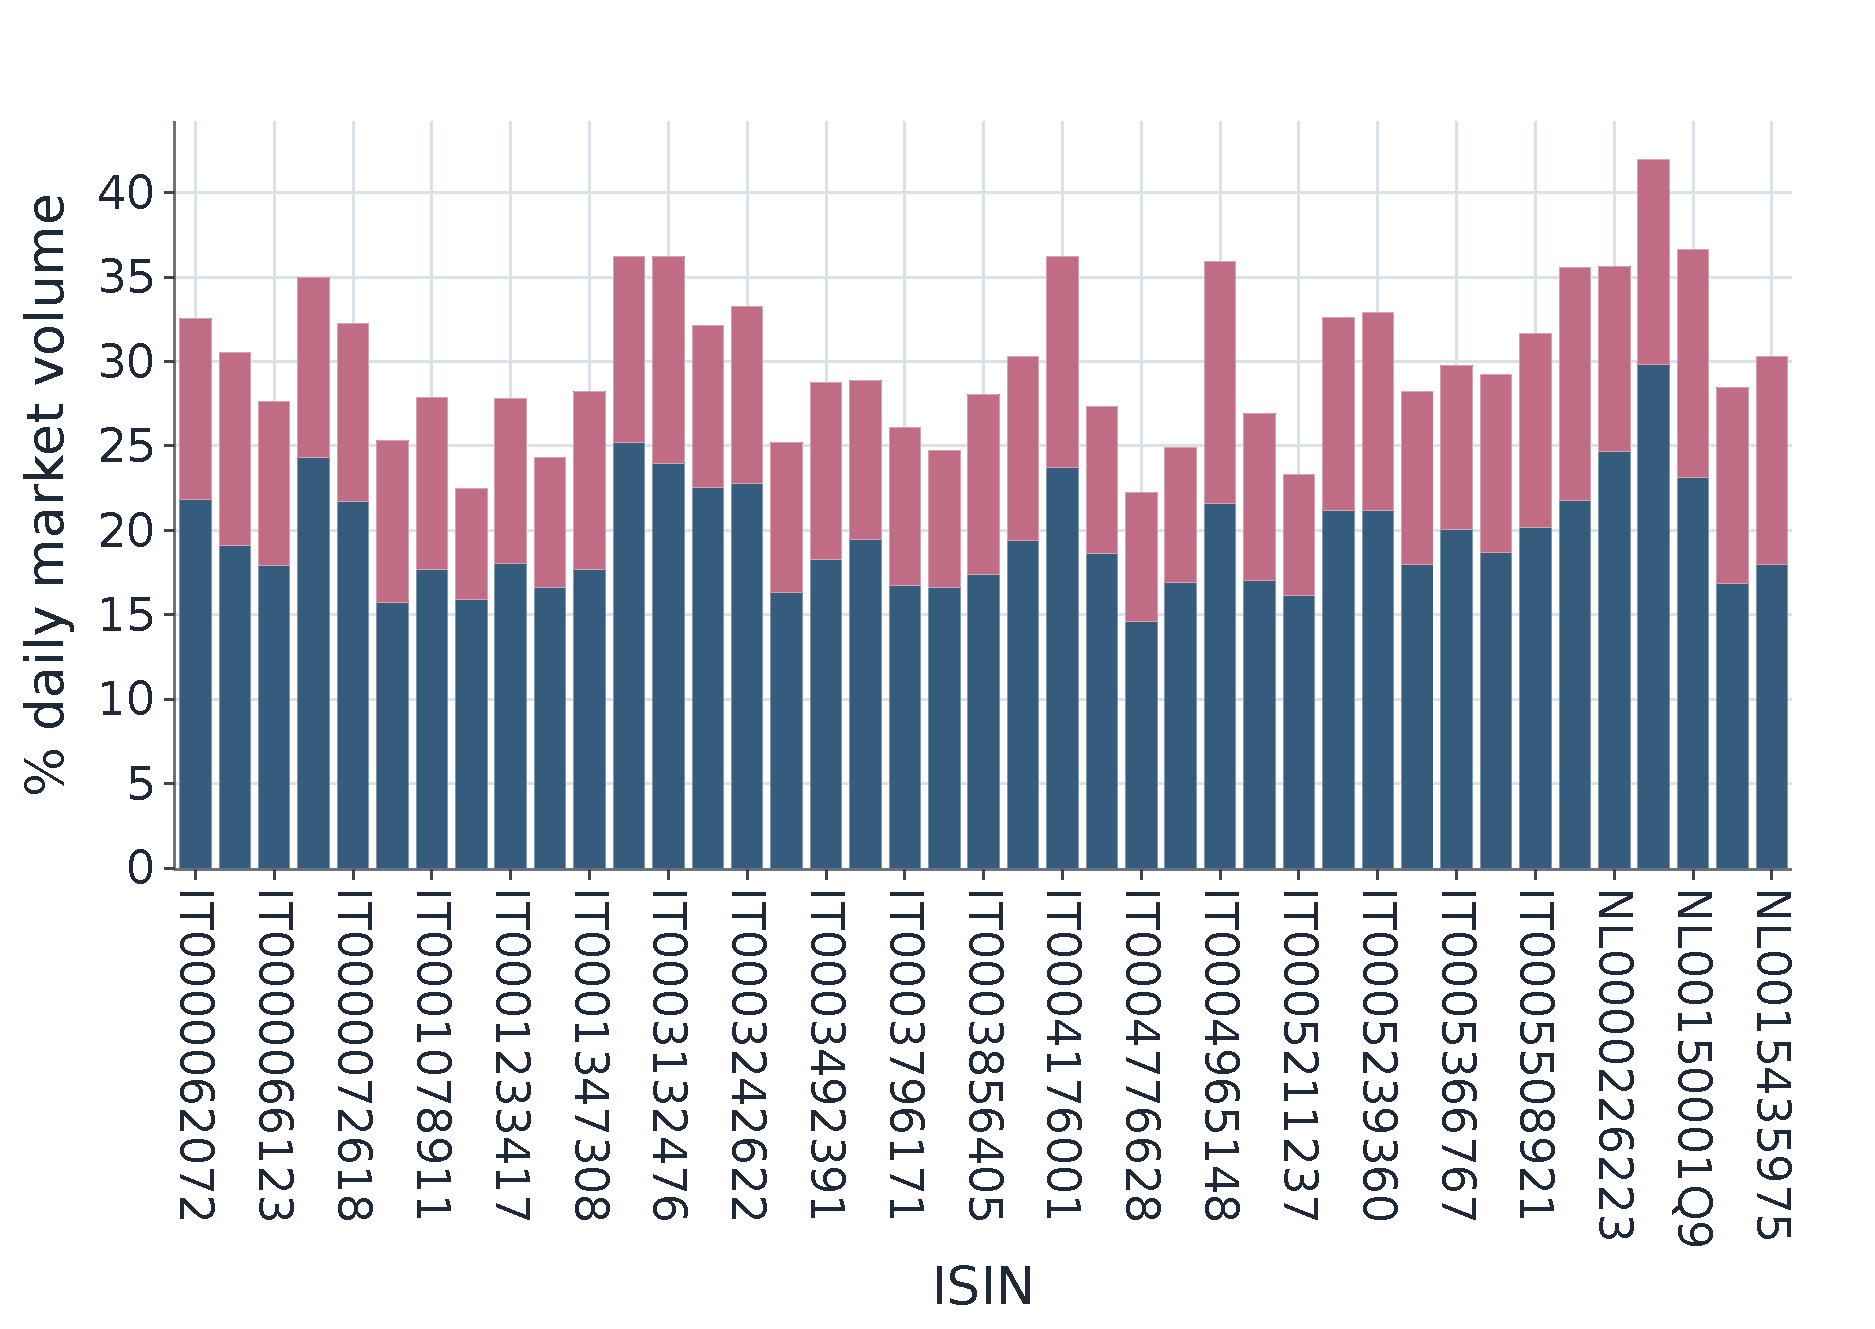
\includegraphics[width=\linewidth]{images/prop_vs_nonprop/png/mean_daily_metaorder_volume_share}
        \caption{Mean percentage of volume within a metaorder with respect to the overall daily volume (blue: proprietary, red: client.)}
        \label{fig:mean_perc_metavol_dailyvol}
    \end{subfigure}
    \caption{}
    \label{fig:member_statistics_combined}
\end{figure}

% \begin{figure}
%     \centering
%     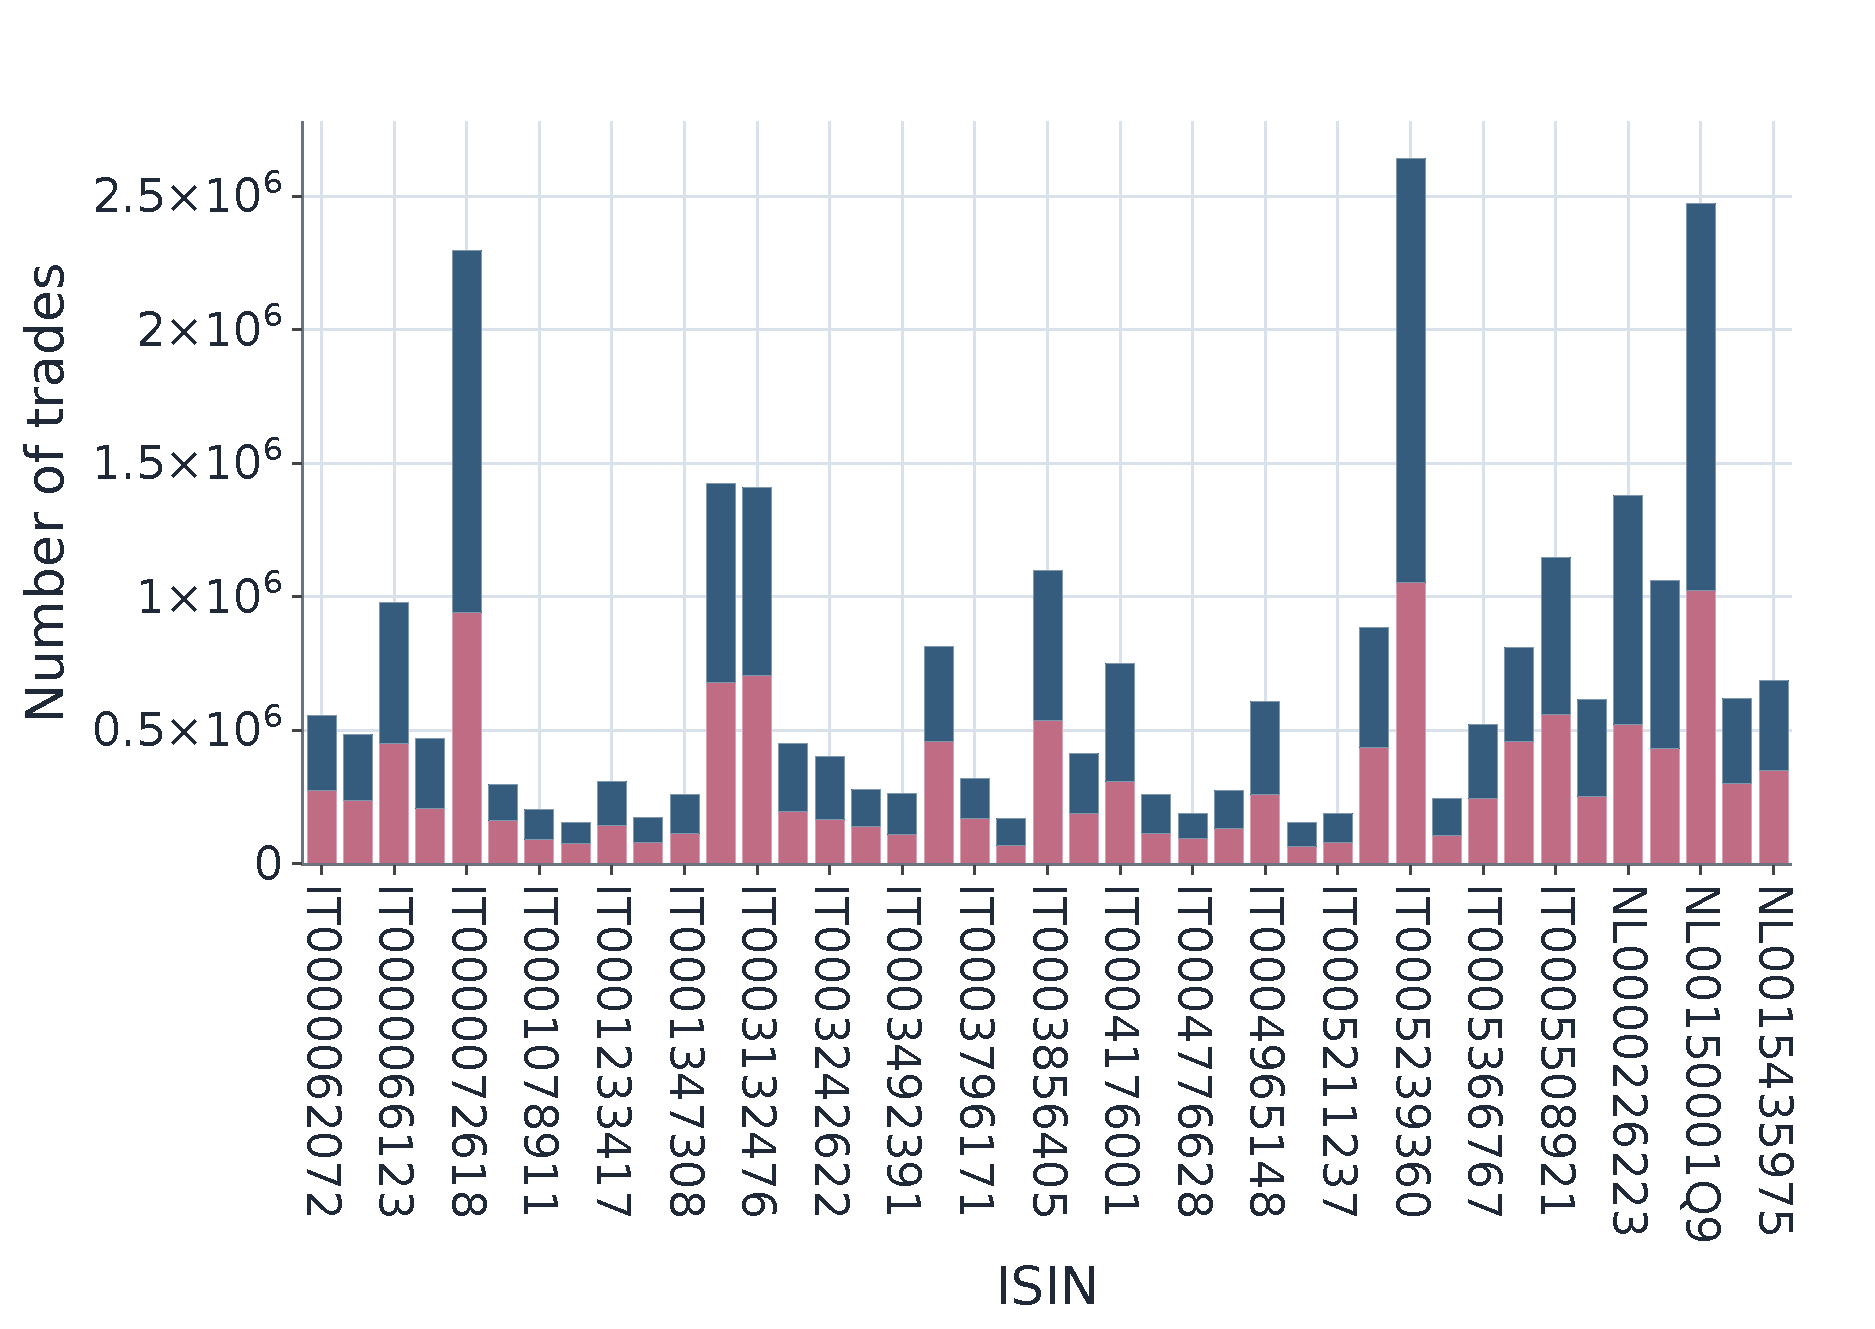
\includegraphics[width=0.8\linewidth]{images/member_statistics/png/proprietary_vs_client_trades_per_isin.png}
%     \caption{Number of proprietary and client trades per ISIN (blue: proprietary, red: client).}
%     \label{fig:prop_vs_client_per_isin}
% \end{figure}

% {\bf Leverei il paragrafo seguente e la figura 3 a meno che non venga richiamata piu' avanti nel testo.} Figure \ref{fig:heatmap_trades} shows the distribution of the number of trades for each member across all the days and 
% all the ISINs in the dataset. Looking at the heatmap, we can notice some vertical bands linked to the most active members 
% during the studied periods, with a little cluster during the first ten days of April 2025 
% \footnote{This period corresponds to the first tarrifs imposed by U.S. president Donal Trump}. An interactive version of this 
% plot can be found in the github repository of the project \cite{repo}.

% \begin{figure}
%     \centering
%     \includegraphics[width=0.8\linewidth]{images/member_statistics/png/member_activity_heatmap.png}
%     \caption{Member-day activity heatmap.}
%     \label{fig:heatmap_trades}
% \end{figure}

\subsection{Metaorder definition at the member level}
Before detailing how we construct metaorders from our dataset, it is useful to briefly review the main approaches that 
have been proposed in the literature to identify such metaorders. Our data set is particularly valuable in this respect, 
as it provides access to both client and member identifiers, as well as detailed information on the nature of each trade. 
These features substantially improve the accuracy of our metaorder reconstruction, placing it just below datasets in which 
metaorders are explicitly labeled. In summary, the literature distinguishes six broad 
categories of metaorder detection methods:

\begin{itemize}
    \item Labelled metaorders: use datasets in which parent orders or execution packages are explicitly reported, so metaorders can be observed directly after applying sample filters
    \cite{zarinelli,BucciEtAl2018,BucciEtAl2020Invariants};

    \item Detection of same-sign sequences from proxies of trader IDs: infer persistent trading agents from available identifier proxies, then group their consecutive aggressive trades with the same sign into candidate metaorders
    \cite{SatoKanazawa2024};

    \item Detection of same-sign sequences from unlabeled member data: reconstruct hidden order splitting by aggregating sequences of same-direction trades associated with the same intermediary, without observing the underlying client identity
    \cite{MoroEtAl2009,VaglicaEtAl2010};

    \item Detection of same-sign sequences from proprietary data with labels on the nature of trades: exploit the distinction between proprietary and client flow to construct and compare metaorders separately across trading categories
    \cite{GomesWaelbroeck2015};

    \item Identification from regimes in the order flow: detect persistent directional regimes or changes in latent order-flow imbalance, and interpret these regimes as periods of coordinated buying or selling pressure
    \cite{Tsaknaki2025};

    \item Synthetic metaorder construction: generate artificial metaorders calibrated to observable market activity when real parent-order identifiers are unavailable, allowing controlled impact analysis under known construction rules
    \cite{MaitrierEtAl2025};
    \end{itemize}


\paragraph{Metaorder construction} We work at the member level: a metaorder is a sequence of
trades routed by a given member, for a given client in a given ISIN and day, with constant sign of
aggressive activity. The construction proceeds as follows.

Fix an instrument $k$ and a member $a$. Let $I_{a,k}$ be the ordered set
of indices $j$ such that member $a$ trades instrument $k$ at time
$t_j \in [09{:}30,17{:}30]$. For each $j \in I_{a,k}$ we observe the
sign $\varepsilon_j$ and volume $q_j$.

We first detect runs of constant sign:
\begin{equation}
  M = \{j_s, j_s+1, \dots, j_e\} \subset I_{a,k}
\end{equation}
such that
\begin{equation}
  \varepsilon_j = \varepsilon_{j_s}, \qquad \forall j \in M,
\end{equation}
and $M$ is maximal with this property (no strictly larger contiguous
set has a constant sign). We apply several filters to the detected sequences. Specifically, we keep only sequences such that
$|M| \geq 5$, all trades in the run belong to the same calendar day, and all trades in the run share the same client identifier. 
This ensures that we do not aggregate orders from different final investors and that we focus on sequences of trades that are likely to be part of the same execution decision.

% \begin{itemize}
% \item  A sequence is kept if $|M|$ $\geq$ 5
%   \item All trades in the run must belong to the same
%         calendar day; runs spanning the market close are discarded.
%   \item All trades in the run share the same
%         client identifier; this ensures that we do not aggregate orders
%         from different final investors.
% \end{itemize}

Even after this step, very long runs can contain long periods of
inactivity. We finally split runs on large gaps. Let $\Delta t_k = t_{j_{k+1}} - t_{j_k}$ be
successive inter-trade gaps within a run. If $\Delta t_k > 1 \text{ hour}$,
the run is split at that point into separate metaorders. Again, 
metaorders with fewer than five trades are discarded. This yields a collection of same-day, same-client, same-sign metaorders for each ISIN.

Each resulting metaorder $i$ is characterised by:

\begin{itemize}
  \item its set of child trades $M_i = \{j_s(i),\dots,j_e(i)\}$,
  \item its sign $\varepsilon_i \in \{+1,-1\}$ (direction), taken as the sign of
        its trades,
  \item its start and end timestamps $t_i^{\text{start}} = t_{j_s(i)}$
        and $t_i^{\text{end}} = t_{j_e(i)}$ defining the execution interval $[t_i^{\text{start}},t_i^{\text{end}}]$,
  \item the capacity flag (proprietary vs client (non-proprietary)).
\end{itemize}

We thus obtain two large metaorder datasets: one for proprietary (group "prop") flow and one for client (group "client") flow
 \footnote{It is crucial to emphasize that a portion of 
  trades labeled as client trades are in fact institutional executions carried out by entities with direct market access 
  on behalf of end-clients who lack such access. These are not retail trades.}, which we analyze 
separately and comparatively in the following sections.

% \begin{itemize}
%   \item proprietary metaorders (group ``prop''),
%   \item client (non-proprietary) metaorders (group ``client'') \footnote{It is crucial to emphasize that a portion of 
%   trades labeled as client trades are in fact institutional executions carried out by entities with direct market access 
%   on behalf of end-clients who lack such access. These are not retail trades.}
% \end{itemize}

Table~\ref{tab:metaorders_numbers} summarises the number of metaorders for each group before and after every filter.

\begin{table}[h!]
\centering
\begin{tabular}{lccc}
\hline
\textbf{Category} & \textbf{Initial Number} & \textbf{After Min Trades} & \textbf{After Min Duration} \\
\hline
Proprietary & 2,774,525 & 866,437 & 588,543 \\
Client      & 988,240  & 308,026 & 256,371 \\
\hline
\end{tabular}
\caption{Metaorder counts for proprietary vs client flow across filtering steps (gap split at 1 hour, min trades set to 5, min duration to 120 seconds).}
\label{tab:metaorders_numbers}
\end{table}

The final dataset contains $588,543$
proprietary metaorders and $256,371$ client metaorders, thus an average of $57$ and $25$ proprietary and client metaorders per day and ISIN, respectively. Buy and sell metaorders are of comparable frequency 
in both groups (proprietary: 279,992 buys vs.\ 308,551 sells; client: 129,919 buys vs.\ 126,452 sells) and the share of daily volume associated with a metaorder ranges between 0.22 and 0.42 with a systematically higher contribution from proprietary metaorders, see Figure \ref{fig:mean_perc_metavol_dailyvol}.

\subsection{Metaorder features}

For each metaorder $i$ we compute:

\begin{itemize}
  \item Metaorder volume
        \begin{equation}
          Q_i = \sum_{j\in M_i} q_j,
        \end{equation}
        i.e.\ the total number of shares executed by the metaorder.

  \item Metaorder direction.
        \begin{equation}
            \varepsilon_i = \begin{cases}
                +1 \quad \text{buy metaorder} \\ -1 \quad \text{sell metaorder}
            \end{cases}
        \end{equation}
  \item Duration
        \begin{equation}
          T_i = t_i^{\text{end}} - t_i^{\text{start}}.
        \end{equation}

  \item Inter-arrival times. Within each metaorder, gaps between
        consecutive child trades are
        \begin{equation}
          \Delta t_i^{(\ell)} = t_{j_{\ell+1}} - t_{j_\ell}, \qquad \ell = 1,\dots, |M_i|-1.
        \end{equation}

\item Average Daily volume.
      In order to smooth day–to–day fluctuations, we consider
      the 5‑day average daily volume
      \begin{equation}
        \bar V_d = \frac{1}{K_d} \sum_{k=0}^{K_d-1} V_{d-k},
      \end{equation}
      where $K_d = 5$  and $V_d$ is the total volume traded in that ISIN on day $d$
      %  \begin{equation}
      %   V_d = \sum_{j \in J_d} q_j,
      % \end{equation}
      % where $J_d$ are all trades in that ISIN on day $d$ {\bf Scritto così pare che sommi solo i volumi dei metaordini, mentre immagino sommi anche i volumi dei trade non dei metaordini}.


  \item Average Daily volatility. For each day, we compute the intraday integrated volatility $\sigma_d$ using a realised-kernel estimator \cite{BarndorffNielsen2008}. Then, we average it similarly as the average daily volume
  \begin{equation}
        \bar{\sigma}_d = \frac{1}{K_d} \sum_{k=0}^{K_d-1} \sigma_{d-k},
  \end{equation}
  The sampling frequency used in the estimation was selected based on the signature plots, choosing the point beyond which the volatility estimates become stable. Using this approach, we decided to sample the data every 1000 seconds. This method differs from the one commonly used in the literature (for example, in \cite{SatoKanazawa2024}), where the volatility is taken as the difference between the opening and closing prices of the day.

  \item Relative size (fraction of daily volume).
        \begin{equation}
          \phi_i = \frac{Q_i}{V_{d(i)}} \in (0,1],
        \end{equation}
        where $d(i)$ denotes the day of metaorder $i$. This is the
        fraction of the daily traded volume executed by the metaorder and enters in the square-root impact law.

  \item Participation rate within the execution window. Let
        $V_i^{\text{window}}$ denote the total market volume
        traded in the same instrument between $t_i^{\text{start}}$ and
        $t_i^{\text{end}}$. The execution participation rate is
        \begin{equation}
          \eta_i = \frac{Q_i}{V_i^{\text{window}}}.
        \end{equation}
        This is the metaorder's market share during its own execution.

  \item Start and end prices. $P_i^{\text{start}}$ and
        $P_i^{\text{end}}$, taken as volume-weighted prices at the
        corresponding timestamps \footnote{A single trade can hit multiple price levels, even if it is rare. In those cases, we consider the volume-weighted price}.

\end{itemize}



\section{Descriptive Properties of Metaorders}
\label{sec:descriptive_properties}

We now present the basic stylised facts about the reconstructed metaorders, focusing on the first research question 
presented in the introduction: Do proprietary and client metaorders differ systematically in their basic execution 
characteristics, such as size, duration, participation rate, and distribution across members? 

Unless stated otherwise, the results are computed at the member 
level and aggregated across ISINs and days. 
% {\bf Molte delle cose che mostri in questa sezione 3 sono note in letteratura 
% (e dovresti dettagliare meglio il confronto quantitativo, ad esempio sugli esponenti di cosa, con quello che si e' 
% osservato in altri mercati). La parte originale di questa sezione (e forse di tutto il paper) e' secondo me il confronto 
% tra metaordini di clienti e proprietari, sui quali pero' non fai molti commenti. La domanda e' quindi "Are the metaorders 
% executed on behalf of clients or on a proprietary basis statistically different?"}

\subsection{Distributions}
In this section, we examine the distributions of several key metrics, most of which will be used in the following 
sections to fit metaorder price impact. For each metric, we consider the decay behaviour of the tail of its distribution. 
Specifically, we apply the power-law fitting procedure introduced in \cite{Clauset_2009}, which is widely regarded as 
the standard approach for fitting power-law models to empirical data and benchmarking them against plausible alternative 
distributions. In our analysis, we compare the power-law fit with lognormal, truncated power-law, and exponential alternatives.

Before turning to the main analysis, it is useful to examine how metaorders are distributed across members and 
whether some members specialize in executing metaorders rather than isolated, sparse trades. Figure 
\ref{fig:metaorders_per_member} addresses both questions. The rank plot of $N_m$ across members is 
broad, revealing a small number of highly active members that execute a very large number of metaorders, 
alongside a long tail of members with much lower metaorder activity. The scatter plot, however, does not 
suggest any clear specialization in metaorder execution. Rather, it indicates that some members execute 
relatively fewer metaorders compared with their overall trading activity than others. This might include, for example, 
market makers.
% {\bf La domanda interessante è se il numero di metaordini di un membro è proporzionale al numero di trades 
% (o al volume) complessivi che ha fatto. In altri termini, l'eterogeneita' di figura 5 e' dovuta al fatto che 
% alcuni membri sono più attivi di altri o riflette una specializzazione di alcuni membri nell'eseguire i metarodini?}

\begin{figure}
    \centering
    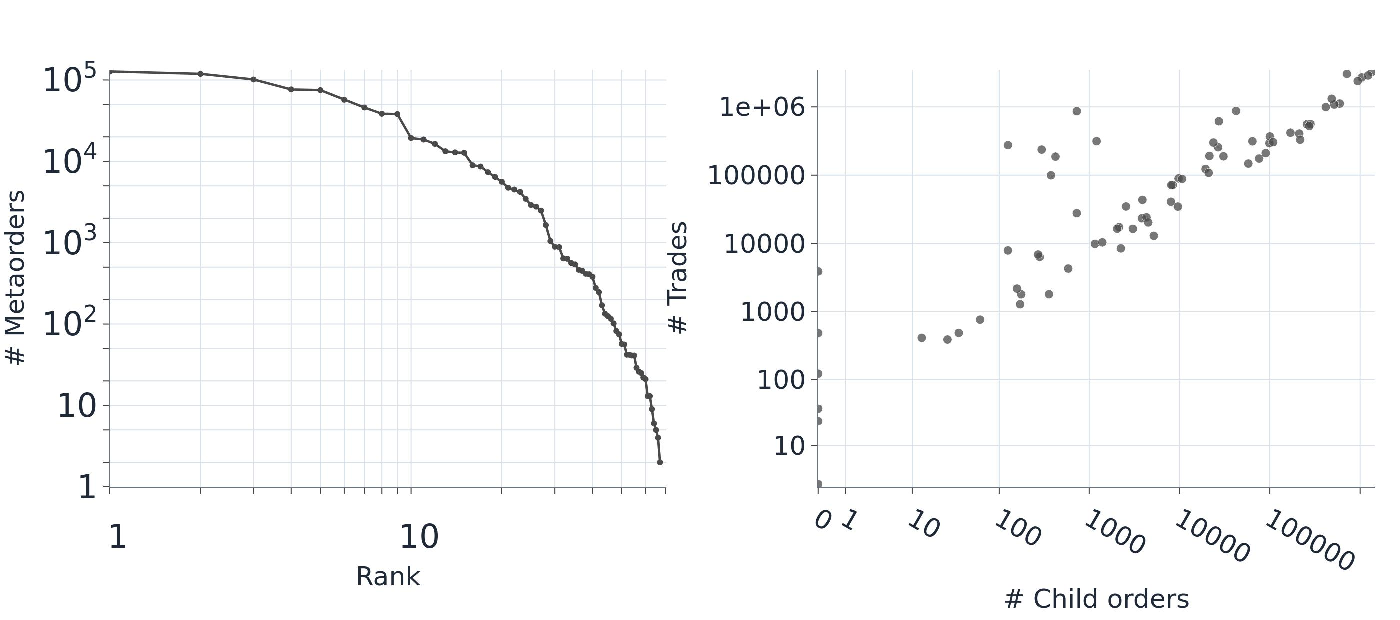
\includegraphics[width=0.8\linewidth]{images/member_metaorder_summary_statistics/png/member_metaorder_profiles_all_metaorders}
    \caption{Log--log rank plot of the number of metaorders per member (left) and zero-preserving log-scaled scatter of the total number of child 
    orders across all metaorders versus the total number of filtered trades at the member level (right).}
    \label{fig:metaorders_per_member}
\end{figure}

We compare the statistical properties of metaorder duration $T$, inter-arrival times $\Delta t$, metaorder volume $Q$, 
and participation rate $\eta$ for client and proprietary metaorders in Figure \ref{fig:metaorders_distributions}.
We observe no striking differences in the statistical properties of the distributions between client and proprietary 
metaorders. The most notable distinction appears in the distribution of participation rates: proprietary metaorders 
tend to shift the mass of the distributoin towardas larger values of $\eta$. Overall, all metrics span several 
orders of magnitude and display heavy-tailed distributions, consistent with the heterogeneous execution 
styles observed in other metaorder datasets 
\cite{MoroEtAl2009,VaglicaEtAl2010,zarinelli}. 

As we can see from Table \ref{tab:best-vs-second-fit} and Figure \ref{fig:metaorders_distributions}, no 
distributions showed an actual power law tail behaviour. For all the metrics, the best fit is either a lognormal 
or a truncated power law model, with a significant tie between the two only for the durations $T$ and relative sizes 
$\phi$ in the case of proprietary metaorders. Table \ref{tab:bootstrap-fit-parameters} reports the fitted parameters 
of the first two best models together with the corresponding percentile bootstrap confidence intervals. However, to compare 
our results with the literature, we overlay on each distribution also the power law fit with the corresponding decaying 
exponent.

\begin{figure}
    \centering
    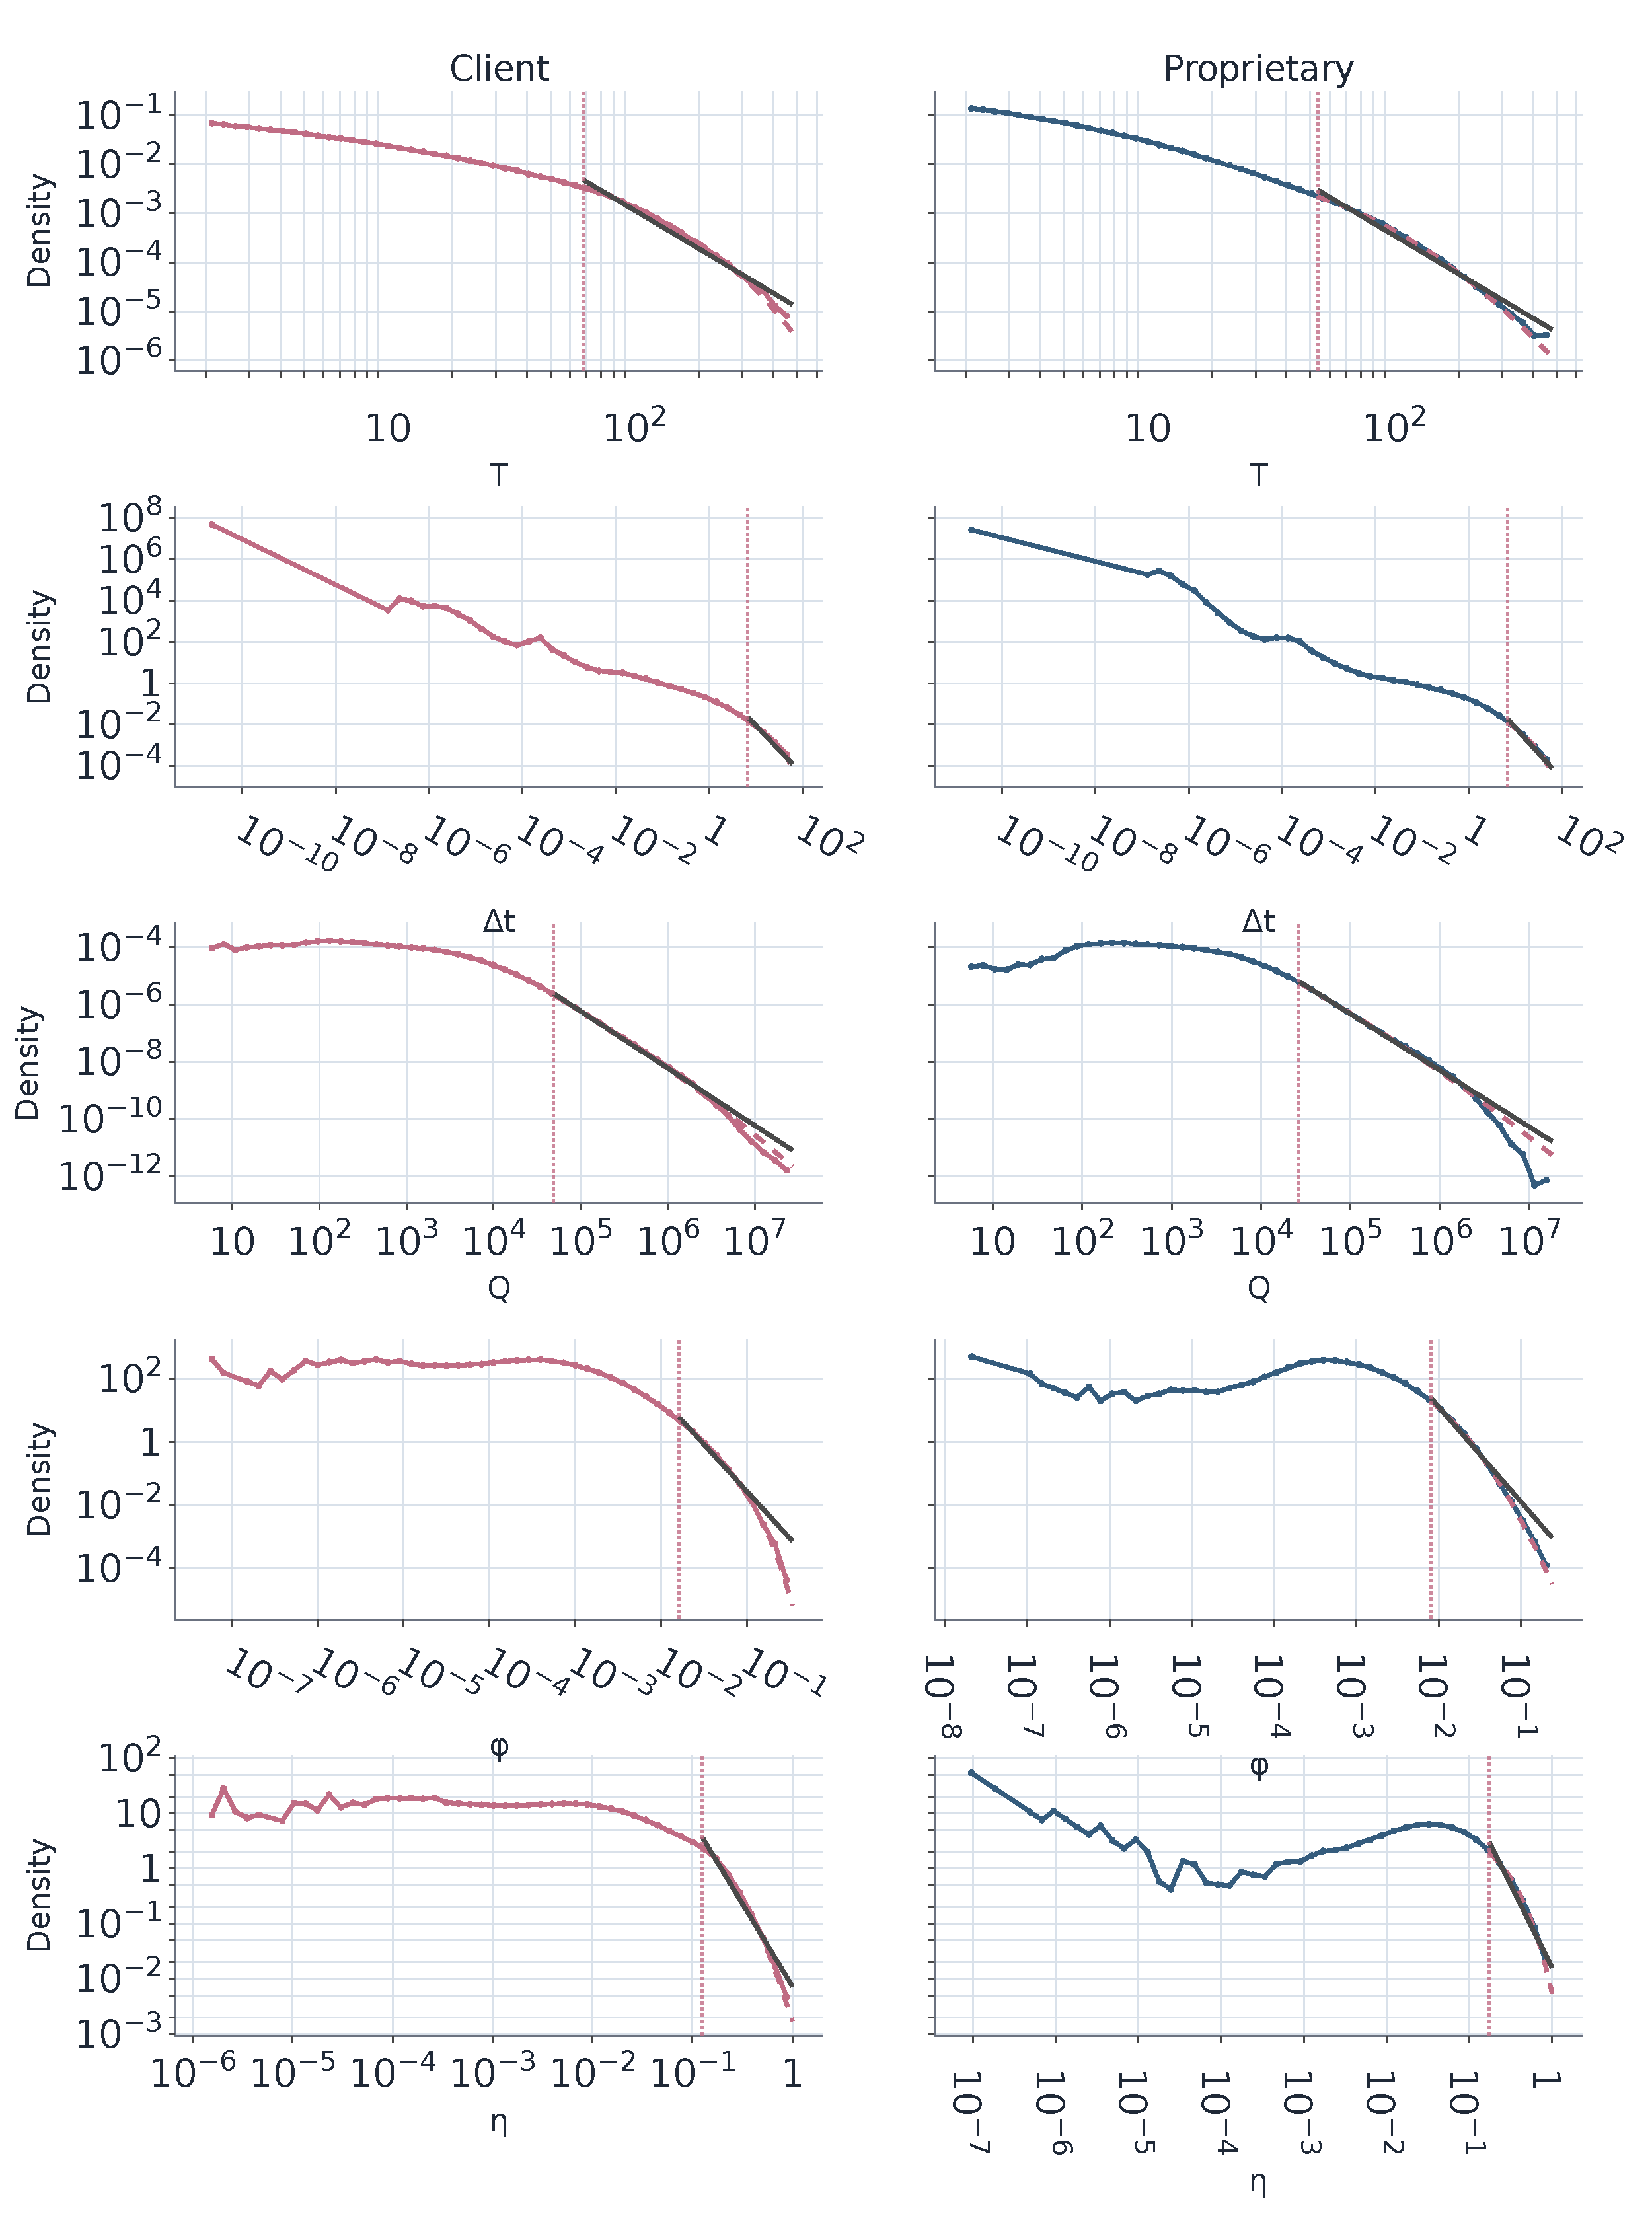
\includegraphics[width=0.9\linewidth]{images/member_metaorder_distributions/png/metaorder_distributions_prop_vs_client}
    \caption{Empirical probability density functions of selected metaorder metrics, conditioned on trading capacity. 
    Vertical dashed lines indicate the estimated lower bound of the power-law regime in the right tail. Solid black 
    lines represent the best power-law fits. The estimated scaling exponents, alongside the statistically preferred 
    model among the tested alternatives, are reported in the legend.}
    \label{fig:metaorders_distributions}
\end{figure}

\begin{table}[htbp]
\centering
\footnotesize
\renewcommand{\arraystretch}{1.15}
\setlength{\tabcolsep}{4pt}

\resizebox{\textwidth}{!}{%
\begin{tabular}{lcccccccc}
\toprule
& \multicolumn{2}{c}{Best Fit by AIC}
& \multicolumn{2}{c}{2nd Best}
& \multicolumn{2}{c}{$\log \dfrac{\mathcal{L}_{1^{\mathrm{st}}}}{\mathcal{L}_{2^{\mathrm{nd}}}}$}
& \multicolumn{2}{c}{p-value} \\
\cmidrule(lr){2-3}
\cmidrule(lr){4-5}
\cmidrule(lr){6-7}
\cmidrule(lr){8-9}
& Client & Proprietary
& Client & Proprietary
& Client & Proprietary
& Client & Proprietary \\
\midrule
$T$
& truncated power law & lognormal
& lognormal & truncated power law
& 47.48 & 4.78
& $\sim 0$ & 0.5511 \\

$\Delta t$
& truncated power law & truncated power law
& lognormal & lognormal
& 2930.58 & 2431.79
& $\sim 0$ & $\sim 0$ \\

$Q$
& truncated power law & truncated power law
& lognormal & lognormal
& 47.53 & 305.10
& $\sim 0$ & $\sim 0$ \\

$Q/V$
& truncated power law & lognormal
& lognormal & truncated power law
& 5.05 & 80.07
& 0.2511 & $\sim 0$ \\

$\eta$
& lognormal & truncated power law
& truncated power law & exponential
& 26.24 & 67.08
& 0.0082 & $\sim 0$ \\
\bottomrule
\end{tabular}%
}
\caption{Best vs second fit review by metric and group. The p values corresponds to the significance test performed on 
the differences in log likehood between the best and second best models. Values below $10^{-5}$ are shown as $\sim 0$.}
\label{tab:best-vs-second-fit}
\end{table}

\begin{table}[htbp]
\centering
\scriptsize
\renewcommand{\arraystretch}{1.15}
\setlength{\tabcolsep}{4pt}

\resizebox{\textwidth}{!}{%
\begin{tabular}{lclcl}
\toprule
Metric & Client model & Client parameters (95\% CI) & Proprietary model & Proprietary parameters (95\% CI) \\
\midrule
$T$
& truncated power law
& \shortstack[l]{$x_{\min}=68.0812\ [62.2530, 68.1113]$\\$\alpha=0.9926\ [0.8344, 1.0501]$\\$\lambda=0.0120\ [0.0115, 0.0130]$}
& lognormal
& \shortstack[l]{$x_{\min}=53.5471\ [48.5295, 52.1330]$\\$\mu=3.5921\ [3.5287, 3.6328]$\\$\sigma=0.7805\ [0.7643, 0.7995]$} \\
\hline
$\Delta t$
& truncated power law
& \shortstack[l]{$x_{\min}=6.5999\ [5.2875, 10.0567]$\\$\alpha=0.9774\ [0.5661, 1.0875]$\\$\lambda=0.0580\ [0.0541, 0.0714]$}
& truncated power law
& \shortstack[l]{$x_{\min}=6.7493\ [6.2979, 8.4972]$\\$\alpha=1.2348\ [1.0791, 1.2727]$\\$\lambda=0.0551\ [0.0537, 0.0605]$} \\
\hline
$Q$
& truncated power law
& \shortstack[l]{$x_{\min}=49139.0000\ [30919.3750, 57036.0000]$\\$\alpha=1.8760\ [1.8548, 1.8905]$\\$\lambda=2.0 \times 10^{-7}\ [1.8 \times 10^{-7}, 2.4 \times 10^{-7}]$}
& truncated power law
& \shortstack[l]{$x_{\min}=26532.0000\ [25076.0750, 32605.9000]$\\$\alpha=1.8598\ [1.8504, 1.8713]$\\$\lambda=3.2 \times 10^{-7}\ [3.0 \times 10^{-7}, 3.5 \times 10^{-7}]$} \\
\hline
$\phi$
& truncated power law
& \shortstack[l]{$x_{\min}=0.0161\ [0.0072, 0.0167]$\\$\alpha=1.9200\ [1.7238, 2.0055]$\\$\lambda=23.9470\ [21.4535, 28.7676]$}
& lognormal
& \shortstack[l]{$x_{\min}=0.0081\ [0.0069, 0.0082]$\\$\mu=-5.7773\ [-5.8757, -5.7264]$\\$\sigma=0.9545\ [0.9367, 0.9801]$} \\
\hline
$\eta$
& lognormal
& \shortstack[l]{$x_{\min}=0.1251\ [0.1147, 0.1258]$\\$\mu=-2.1999\ [-2.2194, -2.1726]$\\$\sigma=0.6815\ [0.6699, 0.6900]$}
& truncated power law
& \shortstack[l]{$x_{\min}=0.1740\ [0.1683, 0.1693]$\\$\alpha=0.3102\ [0.2961, 0.3661]$\\$\lambda=6.4970\ [6.3697, 6.5553]$} \\
\bottomrule
\end{tabular}%
}
\caption{Preferred-model parameter estimates by metric and group, together with the estimated lower cutoff $x_{\min}$.
Confidence intervals are percentile bootstrap intervals at the 95\% level from the nonparametric full-sample
bootstrap with 50 replicates; each replicate re-estimates the lower cutoff and refits all candidate models.}
\label{tab:bootstrap-fit-parameters}
\end{table}


\begin{table}[htbp]
\centering
\scriptsize
\renewcommand{\arraystretch}{1.15}
\setlength{\tabcolsep}{4pt}

\begin{tabular}{lcccccc}
\toprule
& \multicolumn{2}{c}{Sample Size}
& \multicolumn{2}{c}{Mean}
& \multicolumn{2}{c}{Median} \\
\cmidrule(lr){2-3}
\cmidrule(lr){4-5}
\cmidrule(lr){6-7}
& Client & Proprietary
& Client & Proprietary
& Client & Proprietary \\
\midrule

$T$
& 256371 & 588543
& 36.8402 & 19.1341
& 19.0411 & 8.8617 \\

$\Delta t$
& 3449403 & 5297419
& 2.7381 & 2.1258
& 0.5665 & 0.4085 \\

$Q$
& 256371 & 588543
& 38933.1611 & 30800.1527
& 7172.0000 & 6519.0000 \\

$Q/V$
& 256371 & 588543
& 0.0042 & 0.0034
& 0.0018 & 0.0018 \\

$\eta$
& 256371 & 588543
& 0.0844 & 0.1362
& 0.0499 & 0.0949 \\
\bottomrule
\end{tabular}%

\caption{Distribution means and medians by metric and group.}
\label{tab:distribution-means-medians}
\end{table}

\subsection{Execution schedule characterization}
\label{subsec:execution_schedule}
The distributional evidence above already points to an important difference
between the two groups: proprietary metaorders display systematically larger
participation rates than client metaorders. Since participation is tightly linked
to execution aggressiveness, this raises a natural question: are the two groups
also characterized by different execution schedules, beyond differences in
size and duration alone? This question is also motivated by the dynamic impact
results of Section~\ref{subsec:impact-paths} that we anticipate here: if proprietary 
impact is more persistent, one possible channel is that proprietary metaorders are 
executed in a different temporal pattern.

To address this point, we store the child-trade schedule of every metaorder.
Let $t_{i,\ell}$ and $q_{i,\ell}$ denote, respectively, the timestamp and size
of child trade $\ell$ of metaorder $i$. Using the previously defined start and
end times $t_i^{\text{start}}$ and $t_i^{\text{end}}$, we define the normalized execution time
of each child trade as
\begin{equation}
  u_{i,\ell} = \frac{t_{i,\ell} - t_i^{\text{start}}}
                    {t_i^{\text{end}} - t_i^{\text{start}}} \in [0,1],
\end{equation}
and its normalized volume weight as
\begin{equation}
  w_{i,\ell} = \frac{q_{i,\ell}}{Q_i}.
\end{equation}
The cumulative execution schedule of metaorder $i$ is then
\begin{equation}
  C_i(u) = \sum_{\ell : u_{i,\ell} \le u} w_{i,\ell},
  \qquad u \in [0,1].
\end{equation}
By construction, $C_i(0)=0$ and $C_i(1)=1$. For descriptive comparison, we
summarize each group $G \in \{\mathrm{prop},\mathrm{client}\}$ by the
pointwise median cumulative schedule
\begin{equation}
  \widetilde C_G(u) = \operatorname{med}_{i \in G} C_i(u).
\end{equation}
For reference, a TWAP execution corresponds to the diagonal $C(u)=u$.

Figure~\ref{fig:execution_schedule_characterization} reports the median
cumulative schedule together with the heatmap of the empirical density of
$C_i(u)$ in a single object: within each panel, the solid line traces the group
median and the dashed diagonal gives the TWAP benchmark. The clearest result is
that both groups are front-loaded relative to TWAP. By $u=0.10$, the median
cumulative fraction is $0.224$ for proprietary metaorders and $0.206$ for
client metaorders. Equivalently, proprietary metaorders reach one quarter of
their final volume at $u \simeq 0.136$, whereas client metaorders reach the
same threshold at $u \simeq 0.151$. This points to somewhat earlier execution
for proprietary flow at the start of the metaorder, but the gap is modest.

The cross-group difference remains small over the rest of the schedule. Around
the middle of the execution, the two median curves are very close, with
$\widetilde C_{\mathrm{prop}}(0.50)=0.549$ and
$\widetilde C_{\mathrm{client}}(0.50)=0.559$. In the second half of the
metaorder, client flow slightly overtakes proprietary flow: by $u=0.75$ the
median cumulative fractions are $0.758$ and $0.776$, and by $u=0.90$ they are
$0.893$ and $0.907$, respectively. We therefore read the evidence as showing
broadly similar schedule shapes, with only a mild tendency for proprietary
metaorders to execute slightly earlier and for client metaorders to catch up
later. Since this subsection is descriptive and does not attach formal
inference to the median-gap estimates, we do not interpret these differences as
evidence of a strong statistical separation between the two groups.

% The strength of this analysis is that it uses the full child-trade path of the
% metaorder sample, rather than a reduced-form scalar statistic, and does so on a
% very large panel of $588{,}334$ proprietary and $255{,}535$ client metaorders.
% At the same time, its main limitation is that it is deliberately descriptive.
% The median curve still pools together heterogeneous names, directions,
% participation rates, and execution motives; for this reason it should not be
% interpreted as a structural estimate of an ``optimal'' schedule. The heatmap in
% Figure~\ref{fig:execution_schedule_characterization} is useful precisely because
% it makes this dispersion visible: behind the median path, execution styles are
% far from homogeneous. We therefore read the schedule evidence as a
% characterization of the temporal footprint of proprietary and client flow, not
% as a causal statement about the origin of the difference.

\begin{figure}[t]
  \centering
  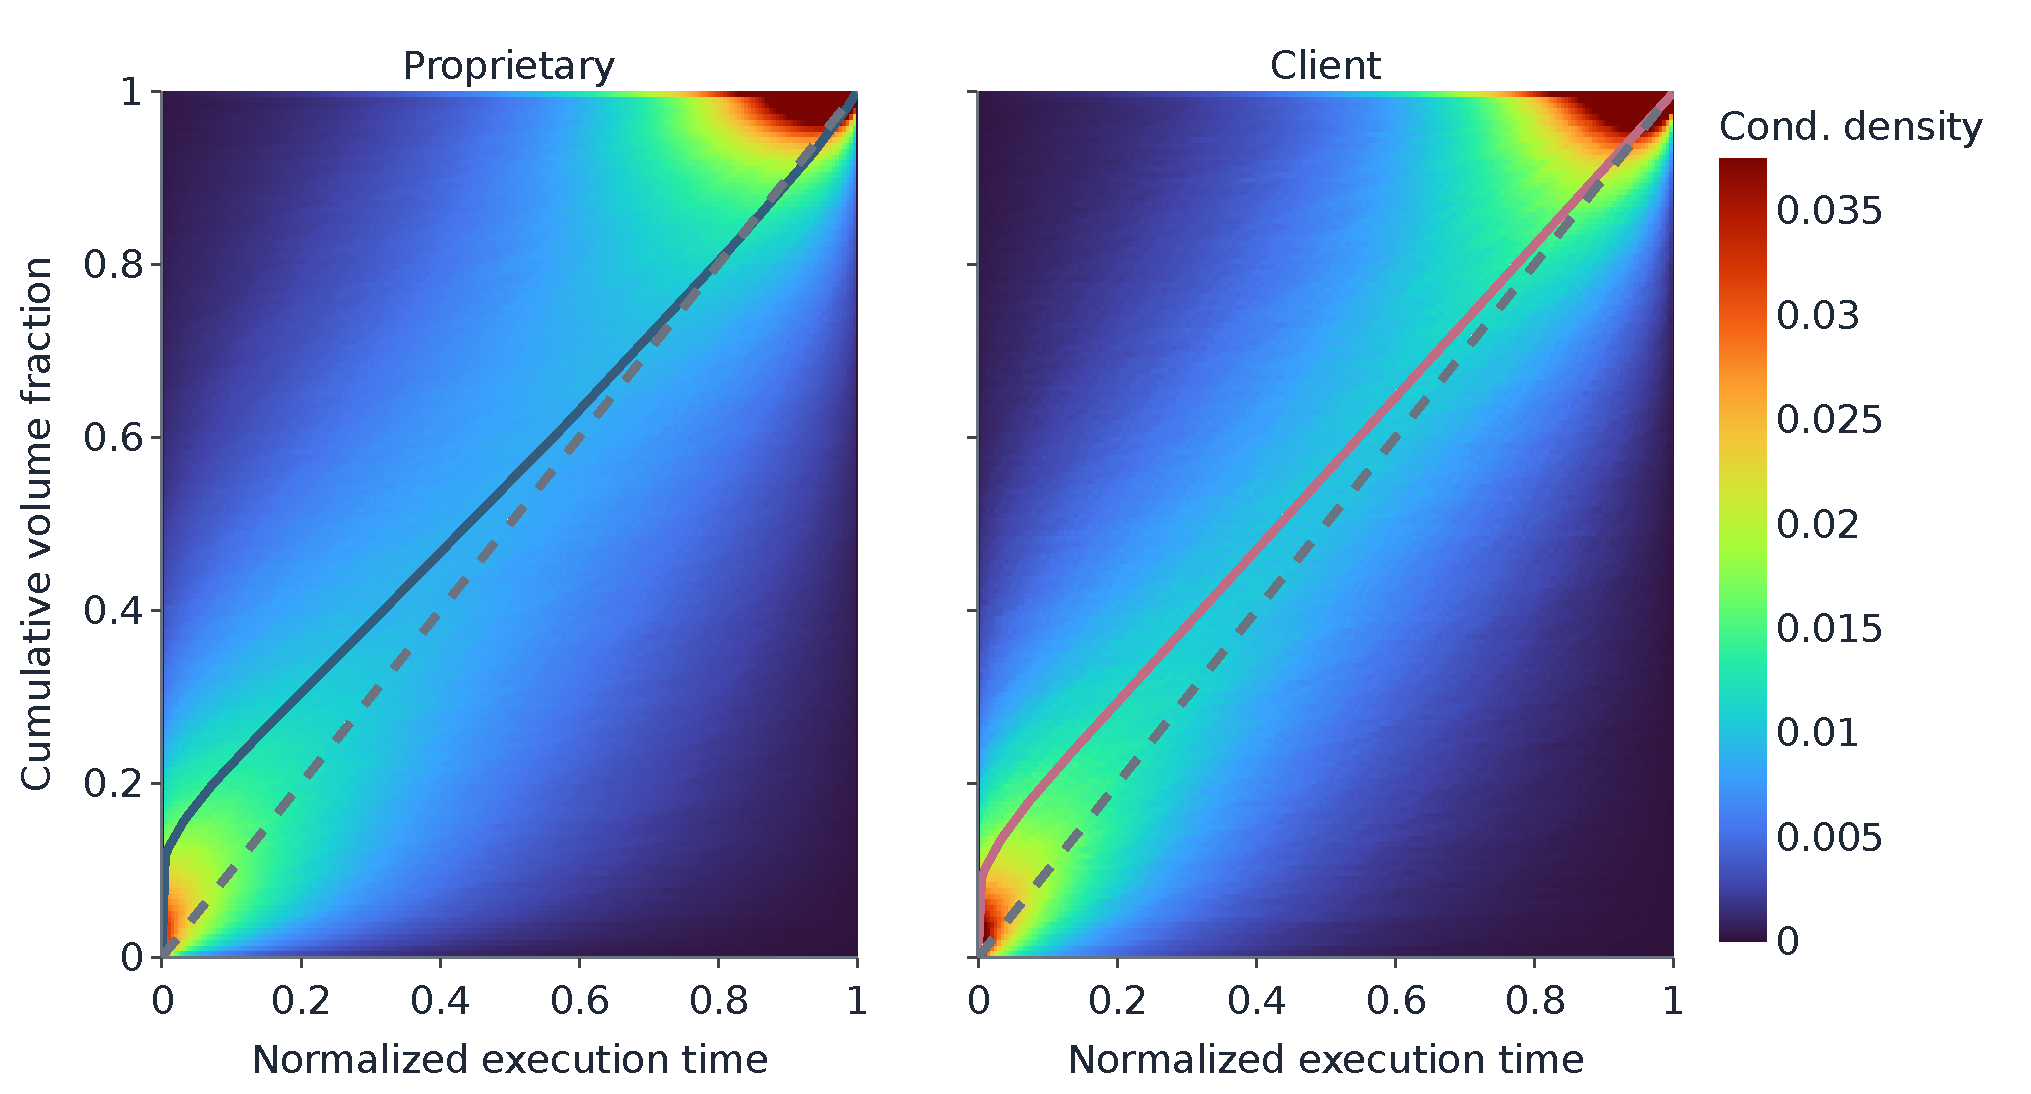
\includegraphics[width=0.94\textwidth]{images/member_metaorder_execution_schedule/png/execution_schedule_heatmap_prop_vs_client_median}
  \caption{Execution schedule characterization at the member level. Left:
  proprietary metaorders. Right: client metaorders. Each panel reports the
  conditional density of cumulative schedules as a function of normalized
  execution time; the solid line overlays the group median cumulative schedule
  and the dashed diagonal is the TWAP benchmark. The heatmap makes the
  cross-sectional heterogeneity around the median path directly visible.}
  \label{fig:execution_schedule_characterization}
\end{figure}

% \subsection{Metaorders per member, durations, and inter-arrival times}
% % Figure \ref{fig:trades_per_member} shows the distribution of the ratio of the ISINs traded over the total number of them for each of the $73$ member. As we can see, almost all the members 
% % traded the majority of the assets, with a very small fraction focused on a smaller subset of the ISINs. {\bf Non capisco perche' mettere qui questa figura; non parla di metaordini e di fatto complementa l'informazione in figura 1, al limite si potrebbe mettere li come pannello destro.}

% % \begin{figure}
% %     \centering
% %     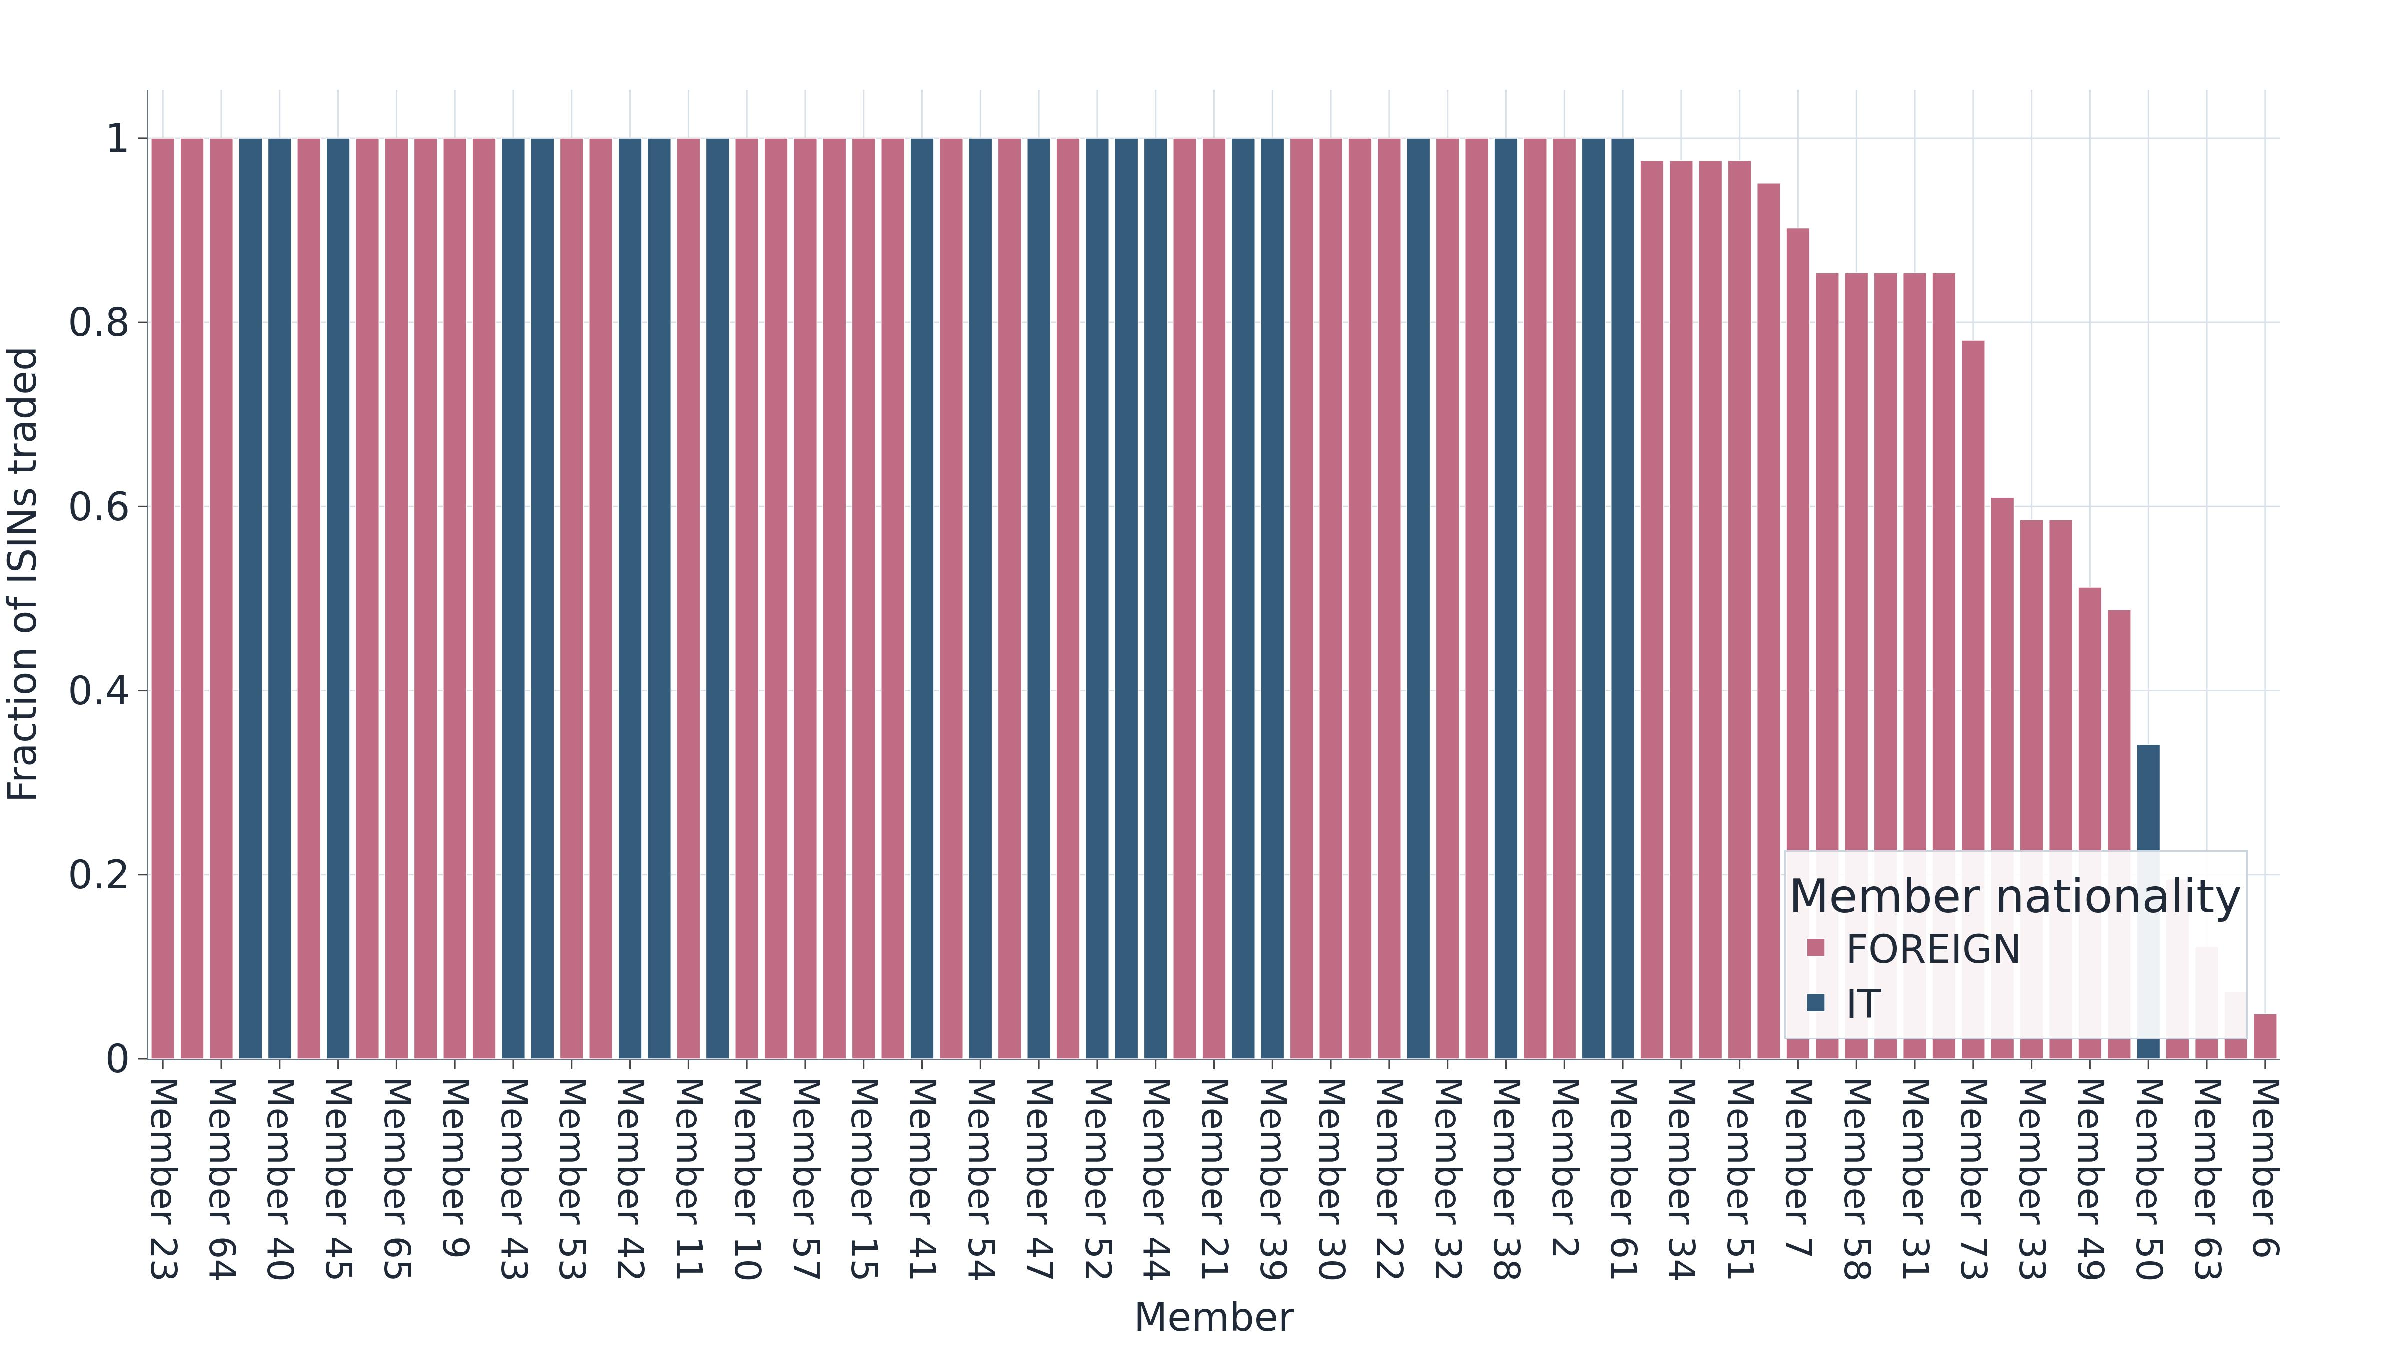
\includegraphics[width=1\linewidth]{images/member_statistics/png/member_isin_coverage_per_member.png}
% %     \caption{Distribution of the fraction of ISINs traded by each member (colors: IT = blue, foreign = red).}
% %     \label{fig:trades_per_member}
% % \end{figure}

% {\bf Per quanto riguarda le figure 5-10, farei un solo pannello con due curve di colori diversi per proprietari e clienti, per aiutare il confronto. Inoltre la qualita' di axis labels e axis ticks andrebbe migliorata. Infine delle scale logaritmiche usare le potenze di 10} Then, we compute the number $N_m$ of metaorders initiated each member $m$.
% %by  count $N_m = \#\{i: \text{metaorder } i \text{ is initiated by } m\}$. 
% The rank plot of $N_m$ across members is broad, with some highly active
% members executing a very large number of metaorders, and a long tail of
% members with fewer metaorders (see Figure \ref{fig:metaorders_per_member}) {\bf La domanda interessante è se il numero di metaordini di un membro è proporzionale al numero di trades (o al volume) complessivi che ha fatto. In altri termini, l'eterogeneita' di figura 5 e' dovuta al fatto che alcuni membri sono più attivi di altri o riflette una specializzazione di alcuni membri nell'eseguire i metarodini?}.

% The distribution of metaorder durations $T_i$ spans several orders of magnitude:
% most metaorders complete within a few minutes, but there is a sizeable
% fraction of longer executions, see Figure \ref{fig:duration} {\bf Qui andrebbe fatto un confronto con la letteratura e una stima dell'esponente di coda della distribuzione.}.
% \begin{figure}[t]
%   \centering
%   \begin{subfigure}{0.7\textwidth}
%     \centering
%     \includegraphics[width=\textwidth]{images/member_non_proprietary/png/metaorder_duration_all.png}
%     \caption{Client}
%   \end{subfigure}
%   \hfill
%   \begin{subfigure}{0.7\textwidth}
%     \centering
%     \includegraphics[width=\textwidth]{images/member_proprietary/png/metaorder_duration_all.png}
%     \caption{Proprietary}
%   \end{subfigure}
%   \caption{Distribution of metaorder durations $T_i$ (in minutes) for
%   client (left) and proprietary (right) flows. Dashed line correspond to the median.}
%   \label{fig:duration}
% \end{figure}
% Within each metaorder, the inter-arrival times between consecutive child
% trades $\Delta t_i^{(\ell)}$ are also broadly distributed, reflecting a
% mixture of rapid sequences of child orders and periods of inactivity, see Figure \ref{fig:interarrival}.
% Even after splitting runs on one-hour inactivity gaps, the distribution remains heavy-tailed, consistent with 
% heterogeneous execution styles documented in other metaorder datasets \cite{MoroEtAl2009,VaglicaEtAl2010,zarinelli}.

% \begin{figure}[t]
%   \centering
%   \begin{subfigure}{0.7\textwidth}
%     \centering
%     \includegraphics[width=\textwidth]{images/member_non_proprietary/png/interarrival_all.png}
%     \caption{Client}
%   \end{subfigure}
%   \hfill
%   \begin{subfigure}{0.7\textwidth}
%     \centering
%     \includegraphics[width=\textwidth]{images/member_proprietary/png/interarrival_all.png}
%     \caption{Proprietary}
%   \end{subfigure}
%   \caption{Distribution of inter-arrival times between child trades within metaorders. Dashed line correspond to the median.}
%   \label{fig:interarrival}
% \end{figure}

Member-nationality conditioning is not part of the main empirical specification. We use the member-nationality label only as an executing-broker diagnostic; the composition table, Italian-member dynamic-impact paths, and Italian-member summary statistics are collected in Appendix~\ref{app:member_nationality_results}.

\section{Impact Model}
\label{sec:impact_model}

To compare metaorders across instruments and dates, we normalise sizes by daily volume and impacts by a daily volatility 
proxy. Building on these normalised quantities, we estimate an average impact law as a function of relative size and 
study how it varies between proprietary and client flow.

\subsection{Instantaneous impact in volatility units}

The peak impact of metaorder $i$ in volatility units is
defined as
\begin{equation}
\label{impact_def}
  I_i = \frac{\varepsilon_i\,\Delta p_i}{\sigma_{d(i)}}.
\end{equation}
By construction, $I_i$ is typically positive on average (buys push the
price up, sells push it down), but individual realisations can be
negative because of noise and concurrent market activity.

Before fitting, we apply a minimum-size filter $\phi_i > 10^{-5}$ to avoid the extremely noisy region of small 
metaorders. We also exclude the few metaorders with participation rate equal to one by imposing $\eta_i < 1$. 
These additional two filters remove, respectively,  $\sim 0.12\%$ and $\sim 0.02\%$ from the entire metaorder 
sample.

This yields a cleaned dataset of $(\phi_i, I_i)$ pairs with auxiliary
features (participation, capacity, etc.) for subsequent analysis.

% Last but not least, we computed the autocorellation function of the signs of the metaorders per ISIN. An example is 
% given in Figure \ref{fig:autocorr_metaorders}.

% \begin{figure}
%     \centering
%     \includegraphics[width=0.8\linewidth]{images/prop_vs_nonprop/png/acf/IT0000062072_acf.png}
%     \caption{Example of autocorrelation of metaorder signs. ISIN IT0000062072 (Generali Assicurazioni SpA)}
%     \label{fig:autocorr_metaorders}
% \end{figure}

\subsection{Impact models}
\label{subsec:impact_models}
Following \cite{zarinelli}, we posit two different functional forms for the relation between the expected 
instantaneous impact and the relative size:
\begin{align}
  \E[I_i \mid \phi_i] &= Y\,\phi_i^\gamma \qquad &\text{Power law} \nonumber \\
  \E[I_i \mid \phi_i] &= a \log_{10}(1+b\phi_i) \qquad &\text{Logarithm}
  \label{eq:impact_model}
\end{align}
where $Y > 0$ is a scale parameter (impact for unit participation), 
$\gamma \in (0,1)$ is the impact exponent (with $\gamma = 1/2$ corresponding to a square-root law 
\cite{BouchaudFarmerLillo2008,SatoKanazawa2024}), and $a, b > 0$ are the parameters of the logarithmic model,
which serves as a benchmark to assess deviations 
from power-law behaviour (e.g. saturation or linear regimes).


Taking logarithms of the power-law specification yields:
\begin{equation}
  \log \E[I_i \mid \phi_i] = \log Y + \gamma \log \phi_i.
\end{equation}

Because individual $I_i$ are noisy and often negative, we do not regress directly on single metaorders. 
Instead we proceed via log-binning.

\paragraph{Binning in relative size.}

We form $K$ logarithmic bins in $\log_{10} \phi$ over the range of the data. For each bin $k$ we compute three quantities.
Specifically, we collect the bin centre $\phi_k$ (e.g.\ geometric mean of $\phi_i$ in the bin), 
the mean impact $\bar{I}_k$ over metaorders in the bin, and the standard error of the mean $\text{SEM}_k$.

% \begin{itemize}
%   \item the bin centre $\phi_k$ (e.g.\ geometric mean of $\phi_i$ in the bin);
%   \item the mean impact $\bar{I}_k$ over metaorders in the bin;
%   \item the standard error of the mean $\text{SEM}_k$.
% \end{itemize}

Bins with fewer than a prescribed minimum count, non-positive or non-finite $\bar{I}_k$, 
or non-finite $\text{SEM}_k$ are discarded.

\paragraph{Estimation procedure: Power Law.}

For the power-law model, we define
\begin{equation}
  X_k = \log \phi_k, \qquad Z_k = \log \bar{I}_k.
\end{equation}
We fit the linear model
\begin{equation}
  Z_k = \alpha + \gamma X_k + \varepsilon_k,
\end{equation}
where $\alpha = \log Y$ and $\gamma$ is the impact exponent. The fit is performed by weighted least squares (WLS) 
in log-space, using weights inversely proportional to the variance of the bin estimate \cite{BouchaudFarmerLillo2008}:
\begin{equation}
    w_k \approx \left(\frac{\bar{I}_k}{\text{SEM}_k}\right)^2.
\end{equation}
Bins with more metaorders and smaller dispersion are given larger weight, while very noisy or poorly populated bins 
contribute less. This yields estimates $\hat{\alpha}$ and $\hat{\gamma}$ together with their standard errors; the 
scale parameter is then recovered as $Y = e^{\hat{\alpha}}$.

\paragraph{Estimation procedure: Logarithmic Benchmark.}

Alongside the power law, we fit the logarithmic specification $\bar{I}_k = a \log_{10}(1+b\phi_k)$ on the same 
binned statistics $(\phi_k, \bar{I}_k)$. Unlike the power law, this model is estimated via a non-linear fit on the 
bin means. Comparing the two curves allows us to visually inspect deviations from the power law, particularly at the 
extremes of the size distribution where the logarithmic form imposes a linear behaviour for $\phi \to 0$ and a slower 
saturation for very large $\phi$.


\paragraph{Empirical impact curves.}

Applying this procedure separately to proprietary and client metaorders yields the impact curves in Figure 
\ref{fig:impact_vs_size_pw}, where the two groups are overlaid in the 
same panel to facilitate comparison. The WLS estimates for the power law specification are:

\begin{itemize}
  \item proprietary: $Y = 0.07264 \pm 0.00366$, $\gamma = 0.3662 \pm 0.0083$;
  \item client: $Y = 0.1281 \pm 0.0154$, $\gamma = 0.5082 \pm 0.0228$.
\end{itemize}
Two differences stand out. First, the scale parameter for client flow is substantially larger than for proprietary 
flow: $Y_{\mathrm{client}}/Y_{\mathrm{prop}} \approx 1.76$. This parameter, however, should not be
read in isolation as a ranking of fitted impact, because the exponent also differs sharply across groups. Since
$\gamma_{\mathrm{prop}} < \gamma_{\mathrm{client}}$, the proprietary curve is flatter in log-log scale and can lie
above the client curve for sufficiently small relative sizes. In the present fit, the two curves cross at about
$\phi^\star \approx 1.9 \times 10^{-2}$: below this threshold, which covers most of the empirical range, proprietary
metaorders have the larger fitted impact; above it, the client curve overtakes. Second, the client exponent is close
to the square-root benchmark, whereas proprietary flow displays a markedly more concave scaling.

For client flow, the logarithmic specification provides an excellent fit  ($R^2 = 0.99$) while the power law remains 
a competitive description ($R^2 = 0.96$). For proprietary flow, by contrast, the power law provides the best fit 
($R^2 = 0.99$) than the logarithmic model ($R^2 = 0.92$). Splitting by side yields very similar parameters for 
proprietary buys and sells, so for brevity we focus on the pooled estimates.


% \begin{table}[t]
%   \centering
%   \small
%   \setlength{\tabcolsep}{6pt}
%   \begin{tabular}{lcc}
%     \toprule
%     Group & Buy $(Y,\gamma)$ & Sell $(Y,\gamma)$ \\
%     \midrule
%     Proprietary & $0.07218 \pm 0.00391$, $0.3699 \pm 0.0090$ & $0.07147 \pm 0.00498$, $0.3589 \pm 0.0114$ \\
%     Client (non-proprietary) & $0.1420 \pm 0.0221$, $0.5311 \pm 0.0303$ & $0.1073 \pm 0.0117$, $0.4695 \pm 0.0201$ \\
%     \bottomrule
%   \end{tabular}
%   \caption{Power-law impact fit parameters split by buy/sell metaorders.}
%   \label{tab:impact_by_side_params}
% \end{table}

The analysis can be refined by conditioning on participation rate
$\eta_i$. Splitting metaorders into quantiles of $\eta_i$ and repeating
the log-binned WLS within each quantile yields a family of impact curves
\[
  \E[I \mid \phi, \eta \in \text{quantile }q] = Y_q \phi^{\gamma_q},
\]
summarized in Figure \ref{fig:impact_by_participation}. 
%and Figure \ref{fig:heatmap_impact_by_participation}.
For proprietary flow, the conditional fits remain close, with a mildly larger exponent at low participation 
($\gamma = 0.38$) than at high participation ($\gamma = 0.35$). For client flow, the dependence on 
participation is much stronger: the low-$\eta$ subset displays a much steeper scaling ($\gamma = 0.84$) than 
the high-$\eta$ subset ($\gamma = 0.39$), so the two conditional curves can cross over the $\phi$ range. This 
behaviour highlights a non-separable interaction between relative size and participation, consistent with the 
joint $(Q/V,\eta)$ dependence reported in \cite{zarinelli}.%, and motivates the bivariate impact surface in 
%Figure~\ref{fig:heatmap_impact_by_participation}.

% \begin{figure}[t]
%   \centering
%   \begin{adjustwidth}{-2.5cm}{-2.5cm}
%     \centering
%     \begin{subfigure}[t]{0.49\linewidth}
%       \centering
%       \includegraphics[width=\linewidth]{images/member_proprietary/png/power_law_fit_overall_member.png}
%       \caption{Proprietary: overall}
%     \end{subfigure}
%     \hfill
%     \begin{subfigure}[t]{0.49\linewidth}
%       \centering
%       \includegraphics[width=\linewidth]{images/member_proprietary/png/power_law_fit_overall_member_by_side.png}
%       \caption{Proprietary: buy vs sell}
%     \end{subfigure}

%     \vspace{0.5em}

%     \begin{subfigure}[t]{0.49\linewidth}
%       \centering
%       \includegraphics[width=\linewidth]{images/member_non_proprietary/png/power_law_fit_overall_member.png}
%       \caption{Client: overall}
%     \end{subfigure}
%     \hfill
%     \begin{subfigure}[t]{0.49\linewidth}
%       \centering
%       \includegraphics[width=\linewidth]{images/member_non_proprietary/png/power_law_fit_overall_member_by_side.png}
%       \caption{Client: buy vs sell}
%     \end{subfigure}
%   \end{adjustwidth}

%   \caption{Average volatility-normalised impact $\bar{I}$ as a function of relative size $\phi = Q/V_d$.
%   Left column: overall fits (power-law with a logarithmic benchmark overlay). Right column: fits split by buy and sell metaorders.
%   Markers are bin-level means with SEM error bars; solid lines are power-law fits and dashed lines are the logarithmic benchmark. 
%   In buy/sell panels: green refers to buys, red refers to sells.}
%   \label{fig:impact_vs_size}
% \end{figure}

\begin{figure}[t]
  \centering
  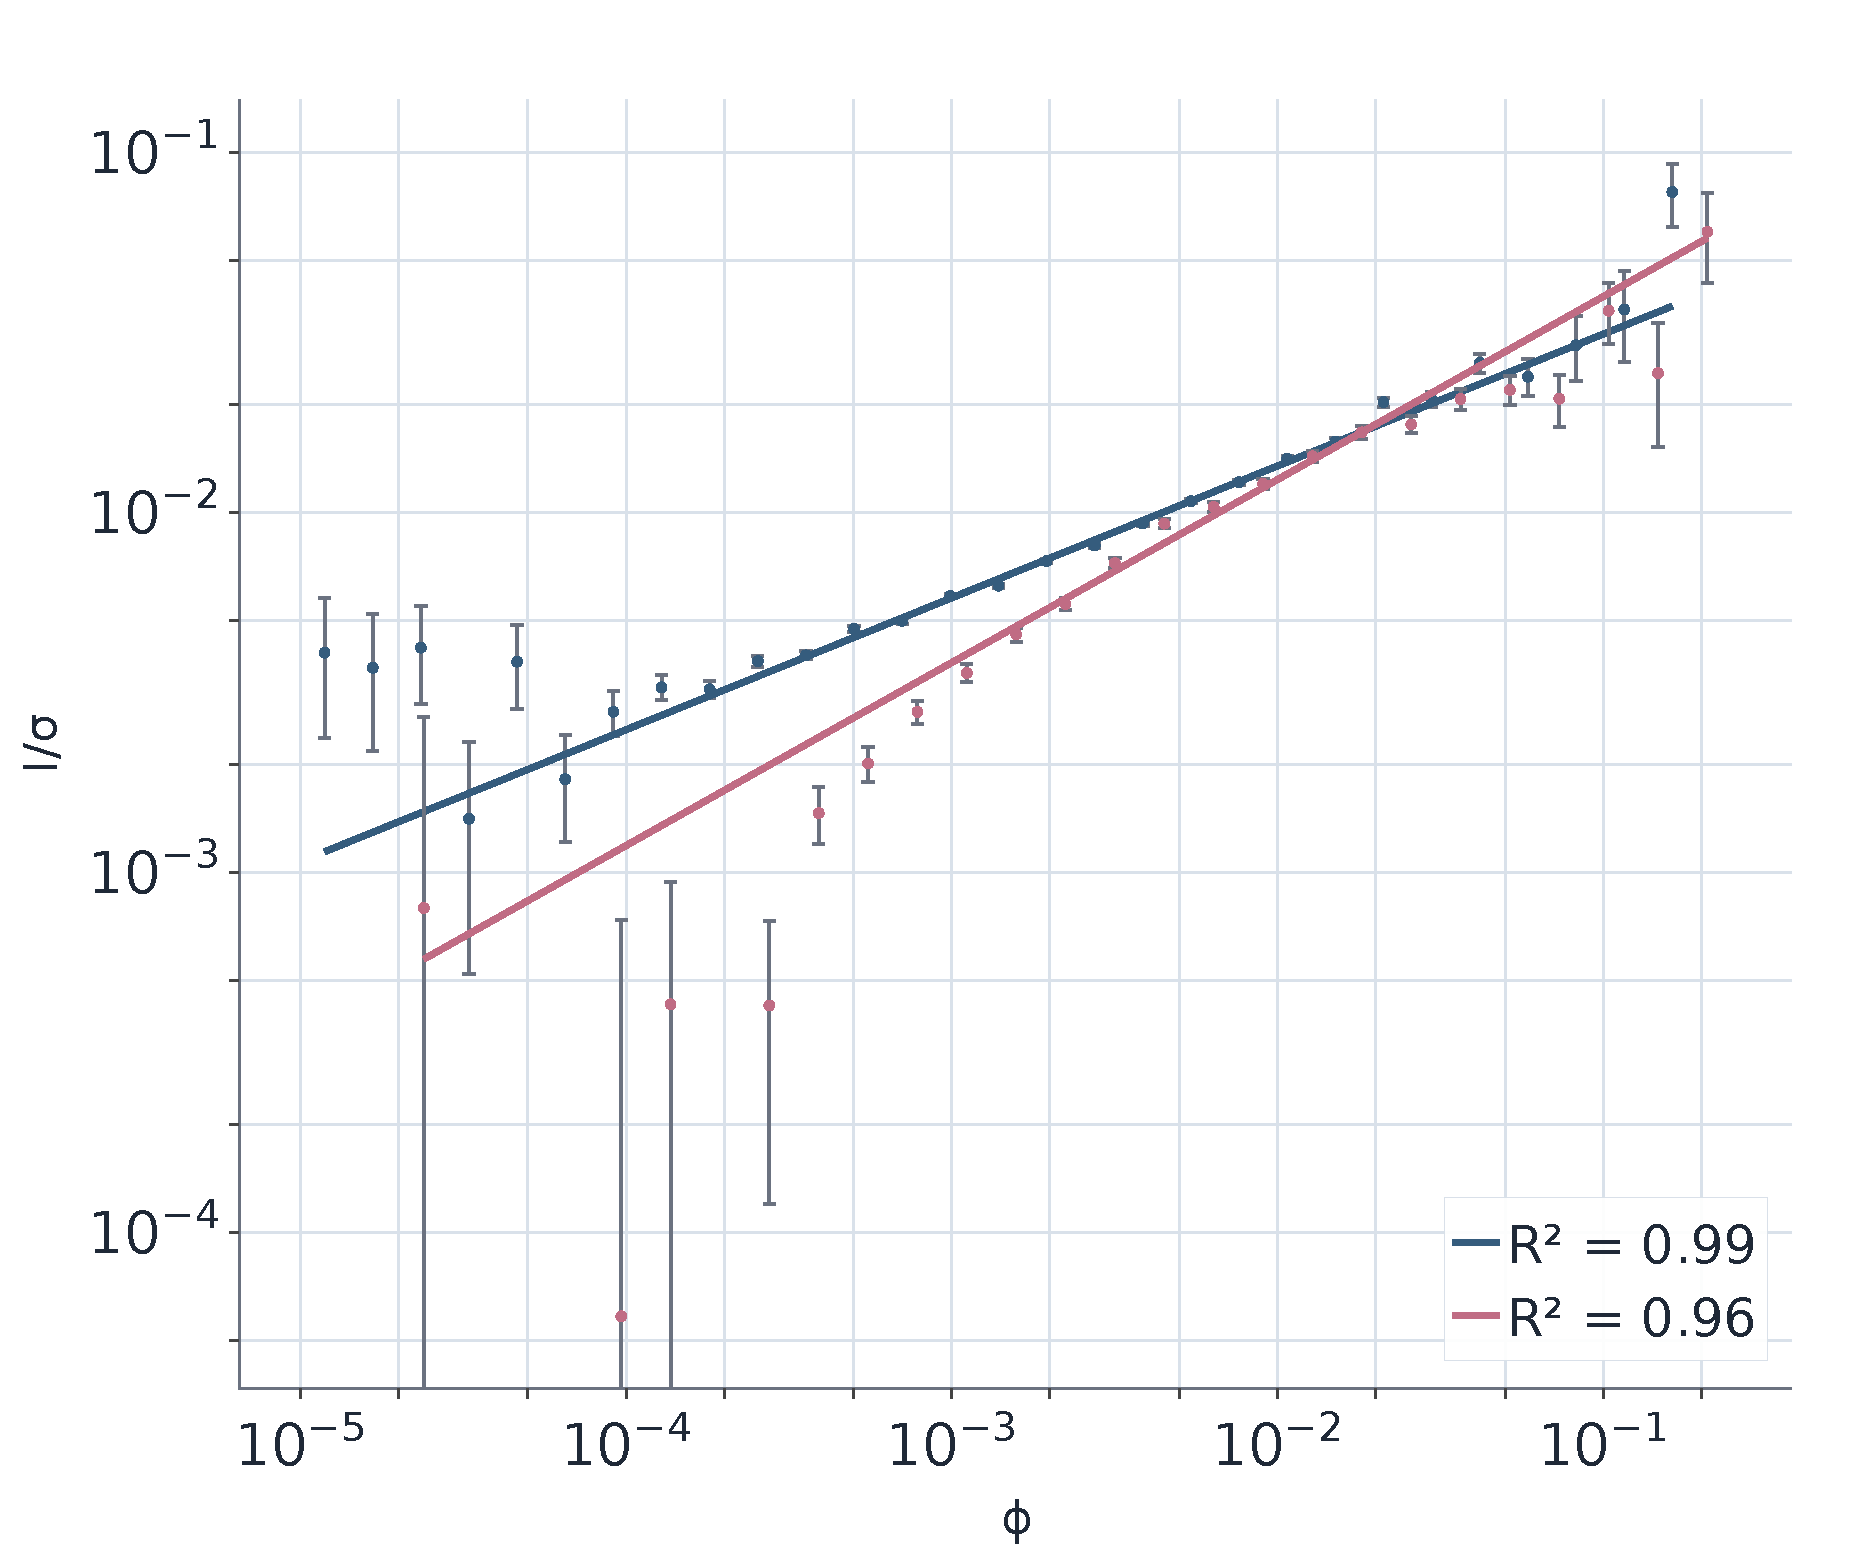
\includegraphics[width=0.480\textwidth]{images/prop_vs_nonprop/png/power_law_prop_vs_nonprop}
  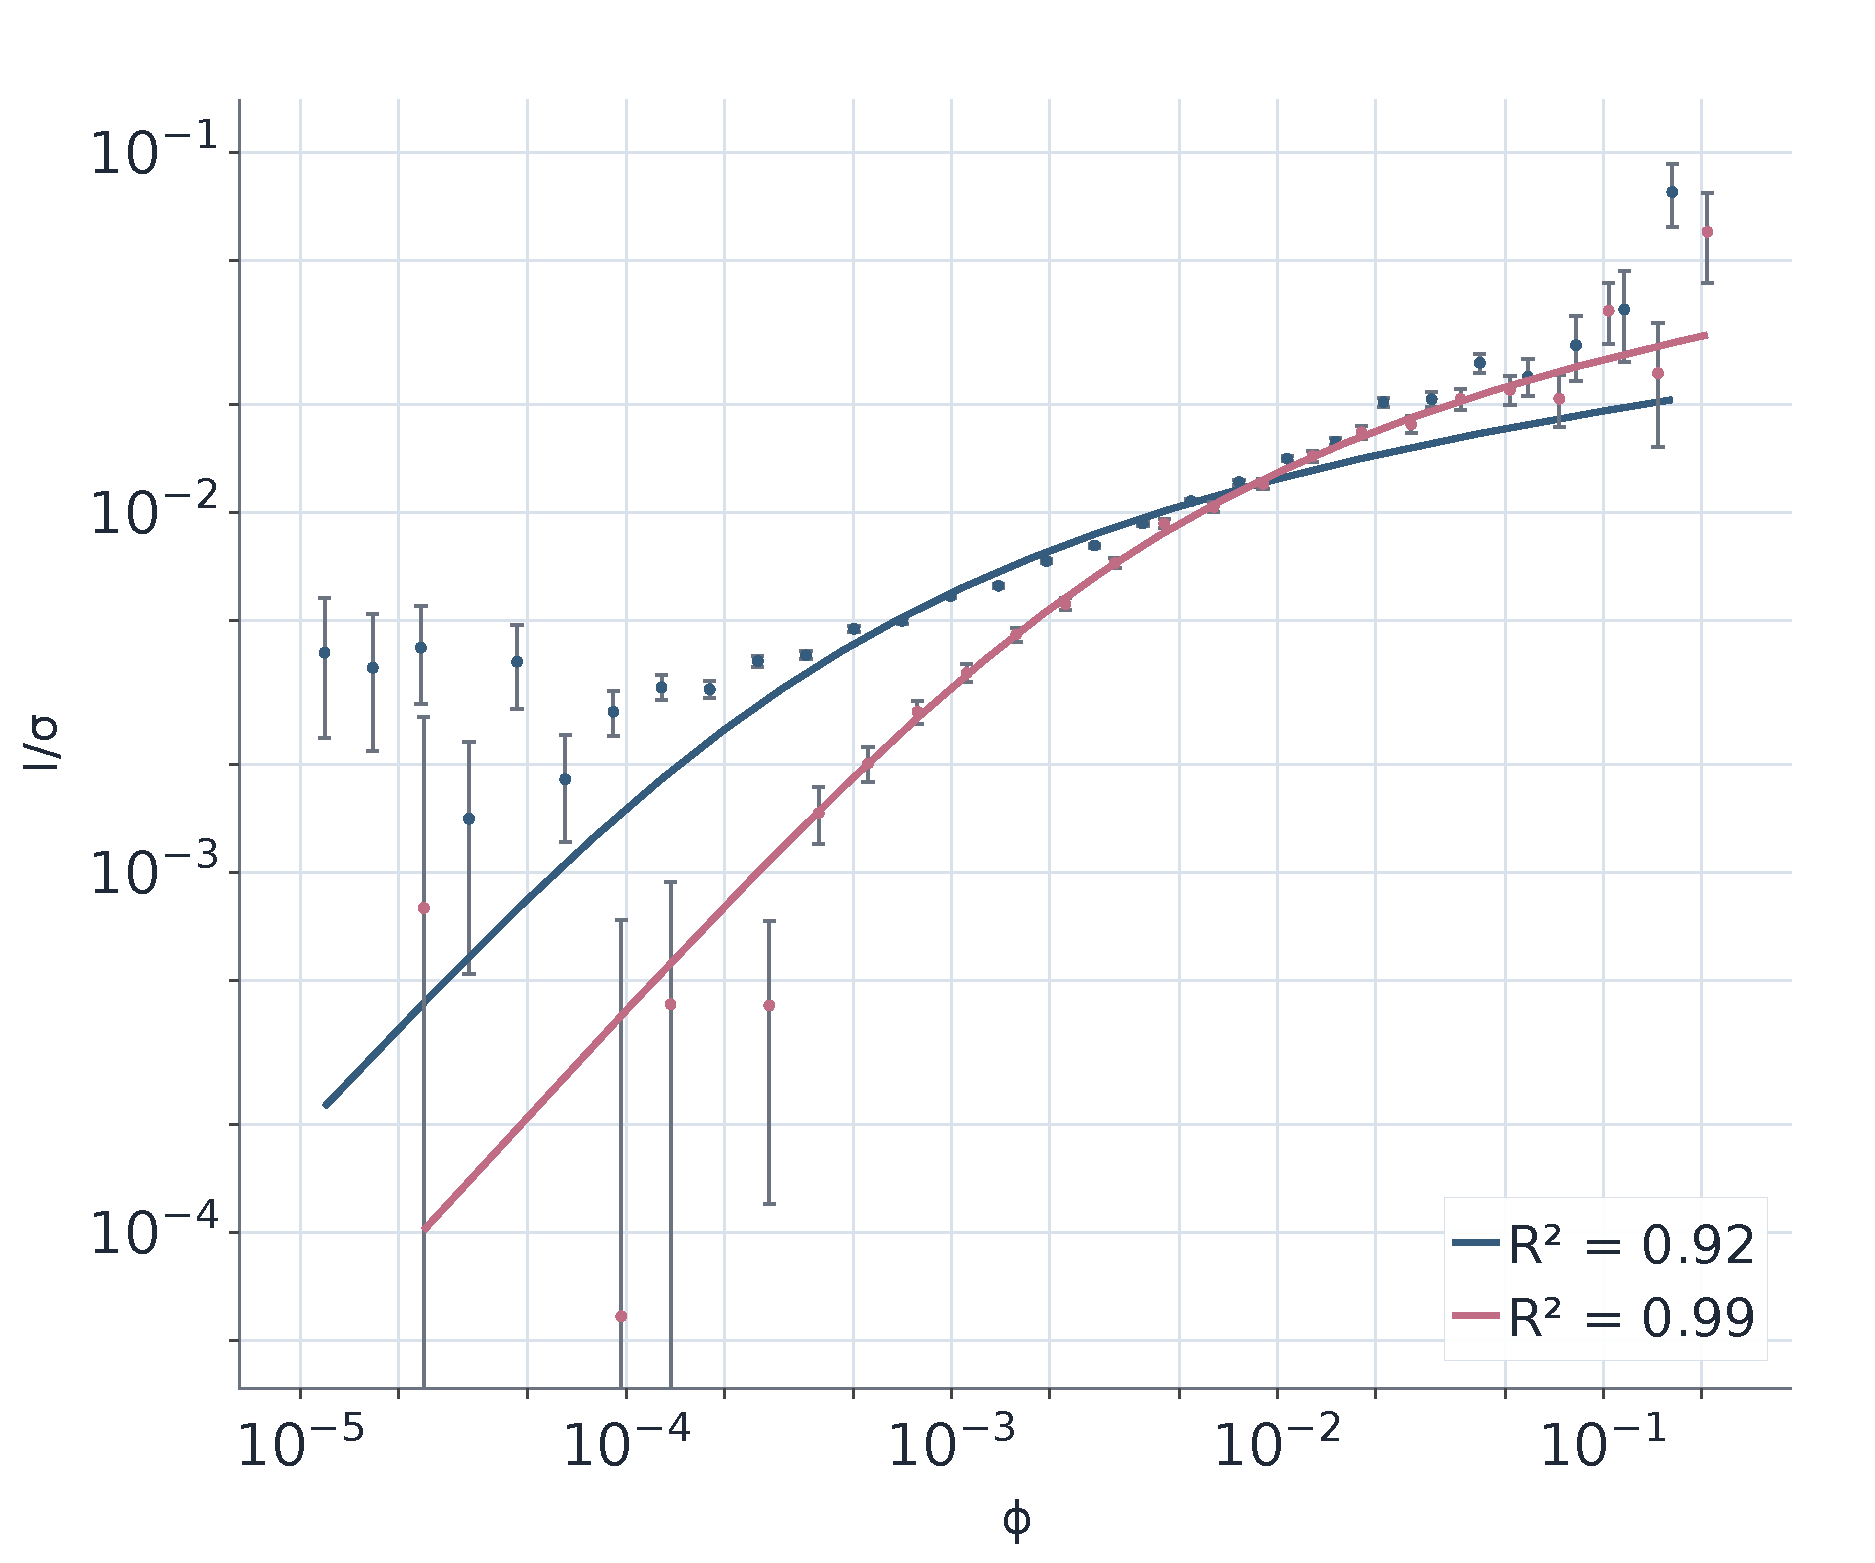
\includegraphics[width=0.480\textwidth]{images/prop_vs_nonprop/png/logarithmic_prop_vs_nonprop}
  \caption{Overlay of proprietary and client overall metaorder impact fits for the power law (left) and logarithmic (right) model (markers: bin means $\pm$ SEM; blue: proprietary, 
  red: client).}
  \label{fig:impact_vs_size_pw}
\end{figure}


\begin{figure}[t]
  \centering
%  \begin{subfigure}[t]{0.48\textwidth}
%    \centering
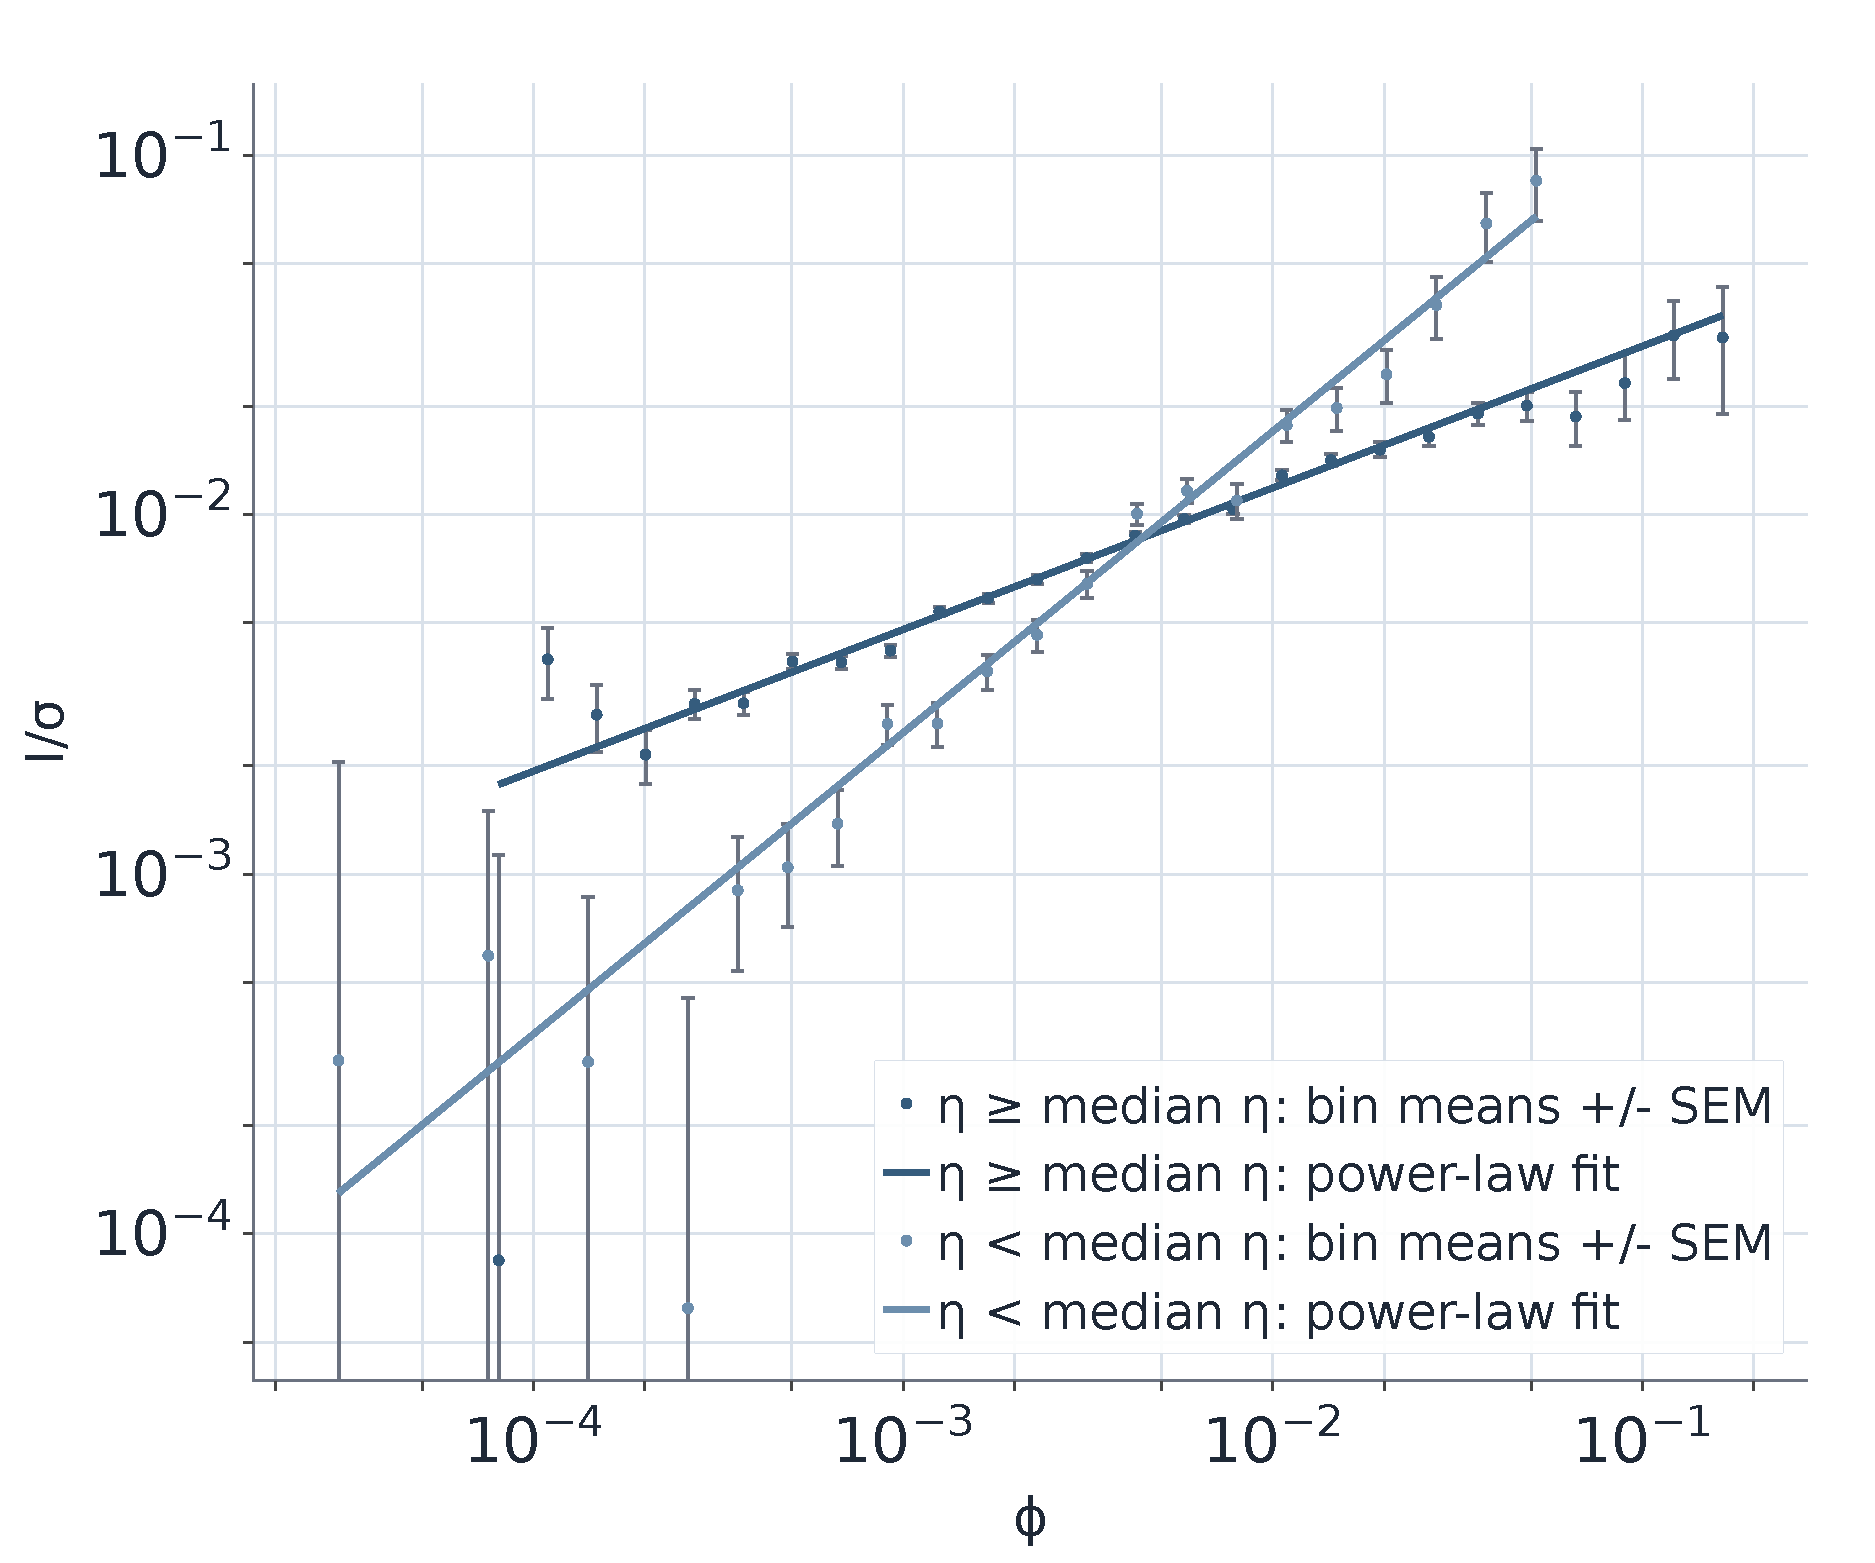
\includegraphics[width=0.480\textwidth]{images/member_non_proprietary/png/power_law_fits_by_participation_rate}   
\includegraphics[width=0.480\textwidth]{images/member_proprietary/png/power_law_fits_by_participation_rate}
%    \caption{Client}
 % \end{subfigure}

%  \vspace{0.7em}

%  \begin{subfigure}[t]{0.4\textwidth}
 %   \centering
%
\includegraphics[width=\linewidth]{images/member_proprietary/png/power_law_fits_by_participation_rate}
%    \caption{Proprietary}
%  \end{subfigure}
  \caption{Impact curves conditional on participation rate median,
  for client (left) and proprietary (right) flow. Each panel shows $\eta < \eta_{\mathrm{median}}$ (green) vs.\ $\eta \ge \eta_{\mathrm{median}}$ (blue)
  subsets; markers are bin means $\pm$ SEM and lines are power-law fits.}
  \label{fig:impact_by_participation}
\end{figure}

\iffalse
\begin{figure}[t]
  \centering
  \begin{adjustwidth}{-2.5cm}{-2.5cm}
    \centering
    \begin{subfigure}[t]{0.515\linewidth}
      \centering
      \includegraphics[width=\linewidth]{images/member_non_proprietary/png/impact_surface_qv_participation_heatmap_member_non_proprietary}
      \caption{Client}
    \end{subfigure}
    \hfill
    \begin{subfigure}[t]{0.48\linewidth}
      \centering
      \includegraphics[width=\linewidth]{images/member_proprietary/png/impact_surface_qv_participation_heatmap_member_proprietary}
      \caption{Proprietary}
    \end{subfigure}
  \end{adjustwidth}
  \caption{Impact surface heatmaps in $(Q/V,\eta)$ for client and proprietary flow (color = mean $I/\sigma$ per bin; empty bins have insufficient observations).}
  \label{fig:heatmap_impact_by_participation}
\end{figure}
\fi

\subsection{Market impact trajectory during and after the execution}
\label{subsec:impact-paths}

The scalar impact measure $I_i$ in the previous section captures only the
price change between the first and last trade of a metaorder. To obtain a time--resolved view of
how impact builds up during execution and relaxes afterwards, we also track the full impact path of
each metaorder.

For a given metaorder $i$ on day $d_i$, using the previously defined start and
end times $t_i^{\text{start}}$ and $t_i^{\text{end}}$ and duration $T_i$, we define the
instantaneous normalised impact at calendar time $t \ge t_i^{\text{start}}$ as
\begin{equation}
  I_i(t) = \frac{\varepsilon_i}{\sigma_{d_i}}\bigl(\log P(t) - \log P_i^{\text{start}}\bigr),
\end{equation}
This is the same normalisation used for
the end-of-execution impact, but evaluated along the whole trajectory of the price process. We then introduce a 
normalised time variable $\tau$ at the metaorder level. During execution,
\begin{equation}
  \tau = \frac{t - t_i^{\text{start}}}{T_i} \in [0,1] \qquad
  (t_i^{\text{start}} \le t \le t_i^{\text{end}}),
\end{equation}
so that $\tau = 0$ corresponds to the first trade and $\tau = 1$ to the last trade. In the
aftermath, we continue to track impact on a time window proportional to the execution duration,
\begin{equation}
  \tau = 1 + \frac{t - t_i^{\text{end}}}{T_i} \in (1, 1 + \lambda],
\end{equation}
for $t_i^{\text{end}} < t \le t_i^{\text{end}} + \lambda T_i$, where $\lambda$ has been fixed to 2. For each metaorder 
we record a partial impact path, i.e.\ the sequence of $I_i(t)$ evaluated after each child
trade during execution ($\tau \in [0,1]$), and an aftermath impact path, i.e.\ $I_i(t)$ sampled at a set of 
evenly spaced times in the interval $(1,1+\lambda]$.
These two vectors are stored per metaorder and subsequently interpolated onto a common normalised time grid 
$\{\tau_m\}_{m=0}^M \subset [0,1+\lambda]$. Averaging across metaorders in a given group $G$ (proprietary or client) 
yields the mean normalised impact path
\begin{equation}
  \bar I_G(\tau_m) = \frac{1}{N_G(\tau_m)} \sum_{i \in G(\tau_m)} I_i(\tau_m),
\end{equation}
where $G(\tau_m)$ is the set of metaorders in group $G$ with a defined impact at time $\tau_m$,
and $N_G(\tau_m) = |G(\tau_m)|$. The sample used here is the same filtered metaorder set as in the
power-law fits (minimum duration, minimum relative size, finite impact).

Figure~\ref{fig:normalized_impact_paths} displays the mean paths for proprietary and client (non-proprietary) metaorders, 
both overall and split by buy/sell. The vertical dashed line marks $\tau = 1$, the end of execution; $\tau > 1$ corresponds 
to the aftermath window.

For client metaorders, the mean impact increases smoothly over the execution interval and peaks at $\tau = 1$. After the end of the execution, the average price relaxes to $\bar I(\tau{=}3)/\bar I(\tau{=}1)\approx 0.57$, 
indicating a sizeable transient component.

For proprietary metaorders the decay is smaller, since $\bar I(\tau{=}3)/\bar I(\tau{=}1)\approx 0.75$. We question the 
null hypothesis of zero differece between the two impact ratios via a bootstrap hypothesis test. We sampled with 
replacement the days within our dataset for 10000 times, recomputing the same difference over each sample. The results 
show that there is no sufficient evidence to accept the null hypothesis ($p<0.001)$. 
This suggests that proprietary metaorders leave a more persistent footprint in prices even if their peak impact is smaller, 
whereas client metaorders are associated with a larger transient component that tends to mean-revert. In line with the literature, the persistent 
component is often  interpreted as a proxy for the information content of the metaorder \cite{GomesWaelbroeck2015}.
Overall, the dynamic profiles are in line with the picture of transient but partly permanent impact emerging from 
empirical studies of metaorders and propagator models: impact accumulates during execution, then relaxes slowly towards 
a non-zero asymptotic level rather than reverting to
zero.
% \footnote{See, for example, the discussion of impact kernels and slow decay in
% Bouchaud, Farmer, and Lillo~\cite{bouchaud2008how}, and the co-impact analysis of
% Bucci et al.~\cite{bucci2020coimpact}, where crowded institutional flows generate persistent price
% moves.} 
In our dataset, the stronger permanence of proprietary impact is consistent with a view in which proprietary trading 
incorporates more information, while client flow is more liquidity-demanding and hence more prone to subsequent partial 
reversal. This dynamic perspective complements the static power-law fits of Section~\ref{subsec:impact_models} and provides 
additional evidence that market impact and its decay depend sensitively on who trades and how their orders are crowded in 
time and across investors.

\begin{figure}[t]
  \centering
  \begin{adjustwidth}{0.01\textwidth}{0.01\textwidth}
    \centering

    \begin{subfigure}[t]{0.48\linewidth}
      \centering
      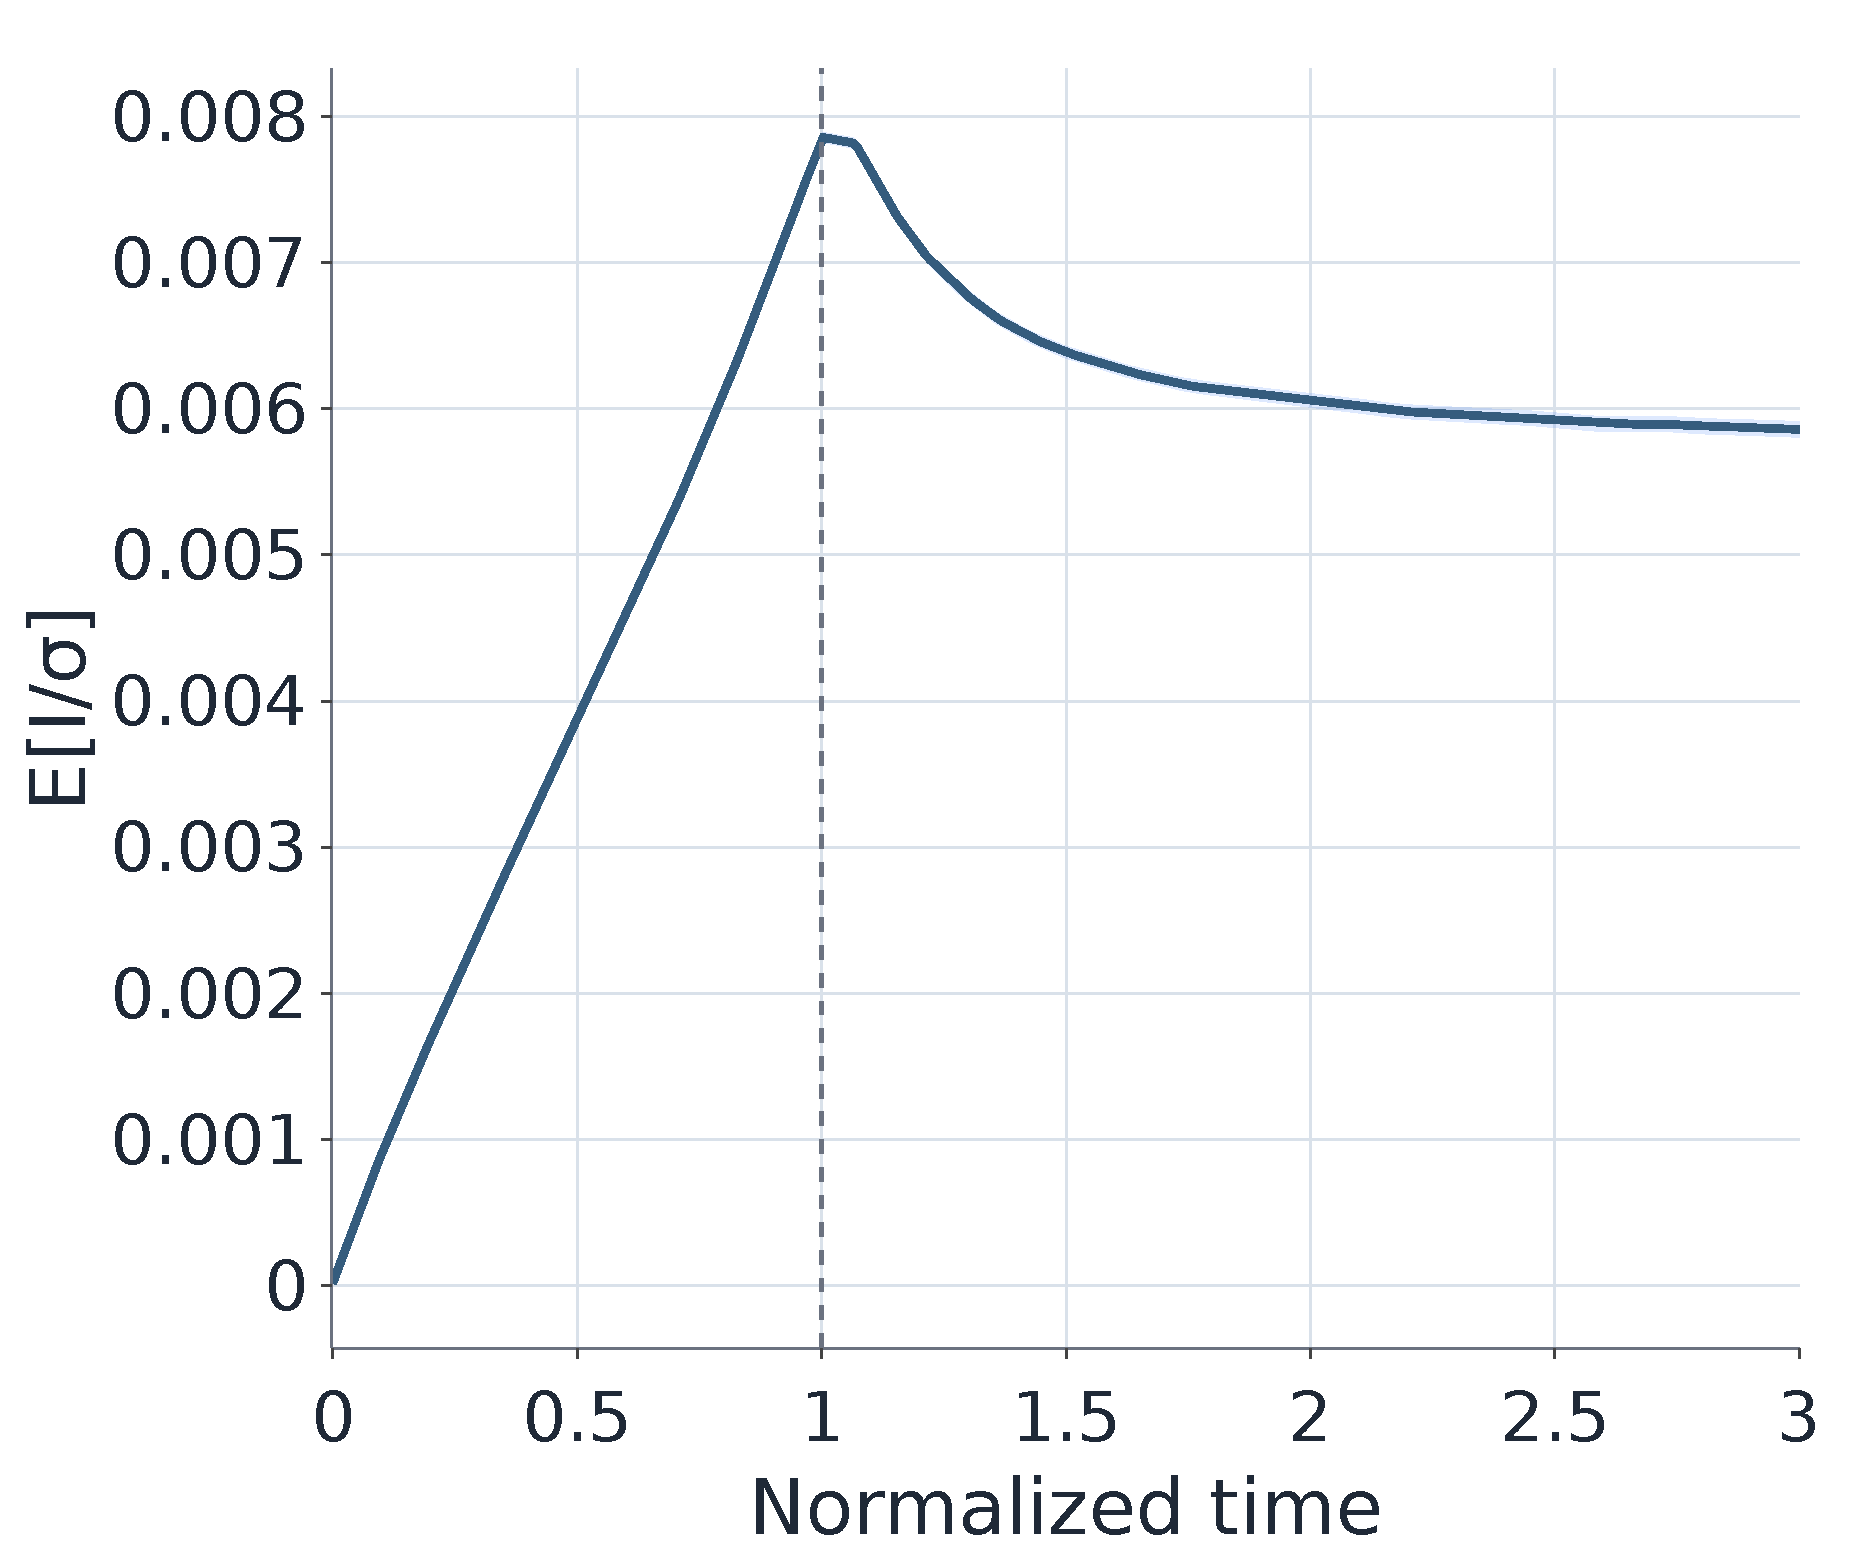
\includegraphics[width=\linewidth]{images/member_proprietary/png/normalized_impact_path_member_proprietary}
      \caption{Proprietary}
    \end{subfigure}
    \hfill
    \begin{subfigure}[t]{0.48\linewidth}
      \centering
      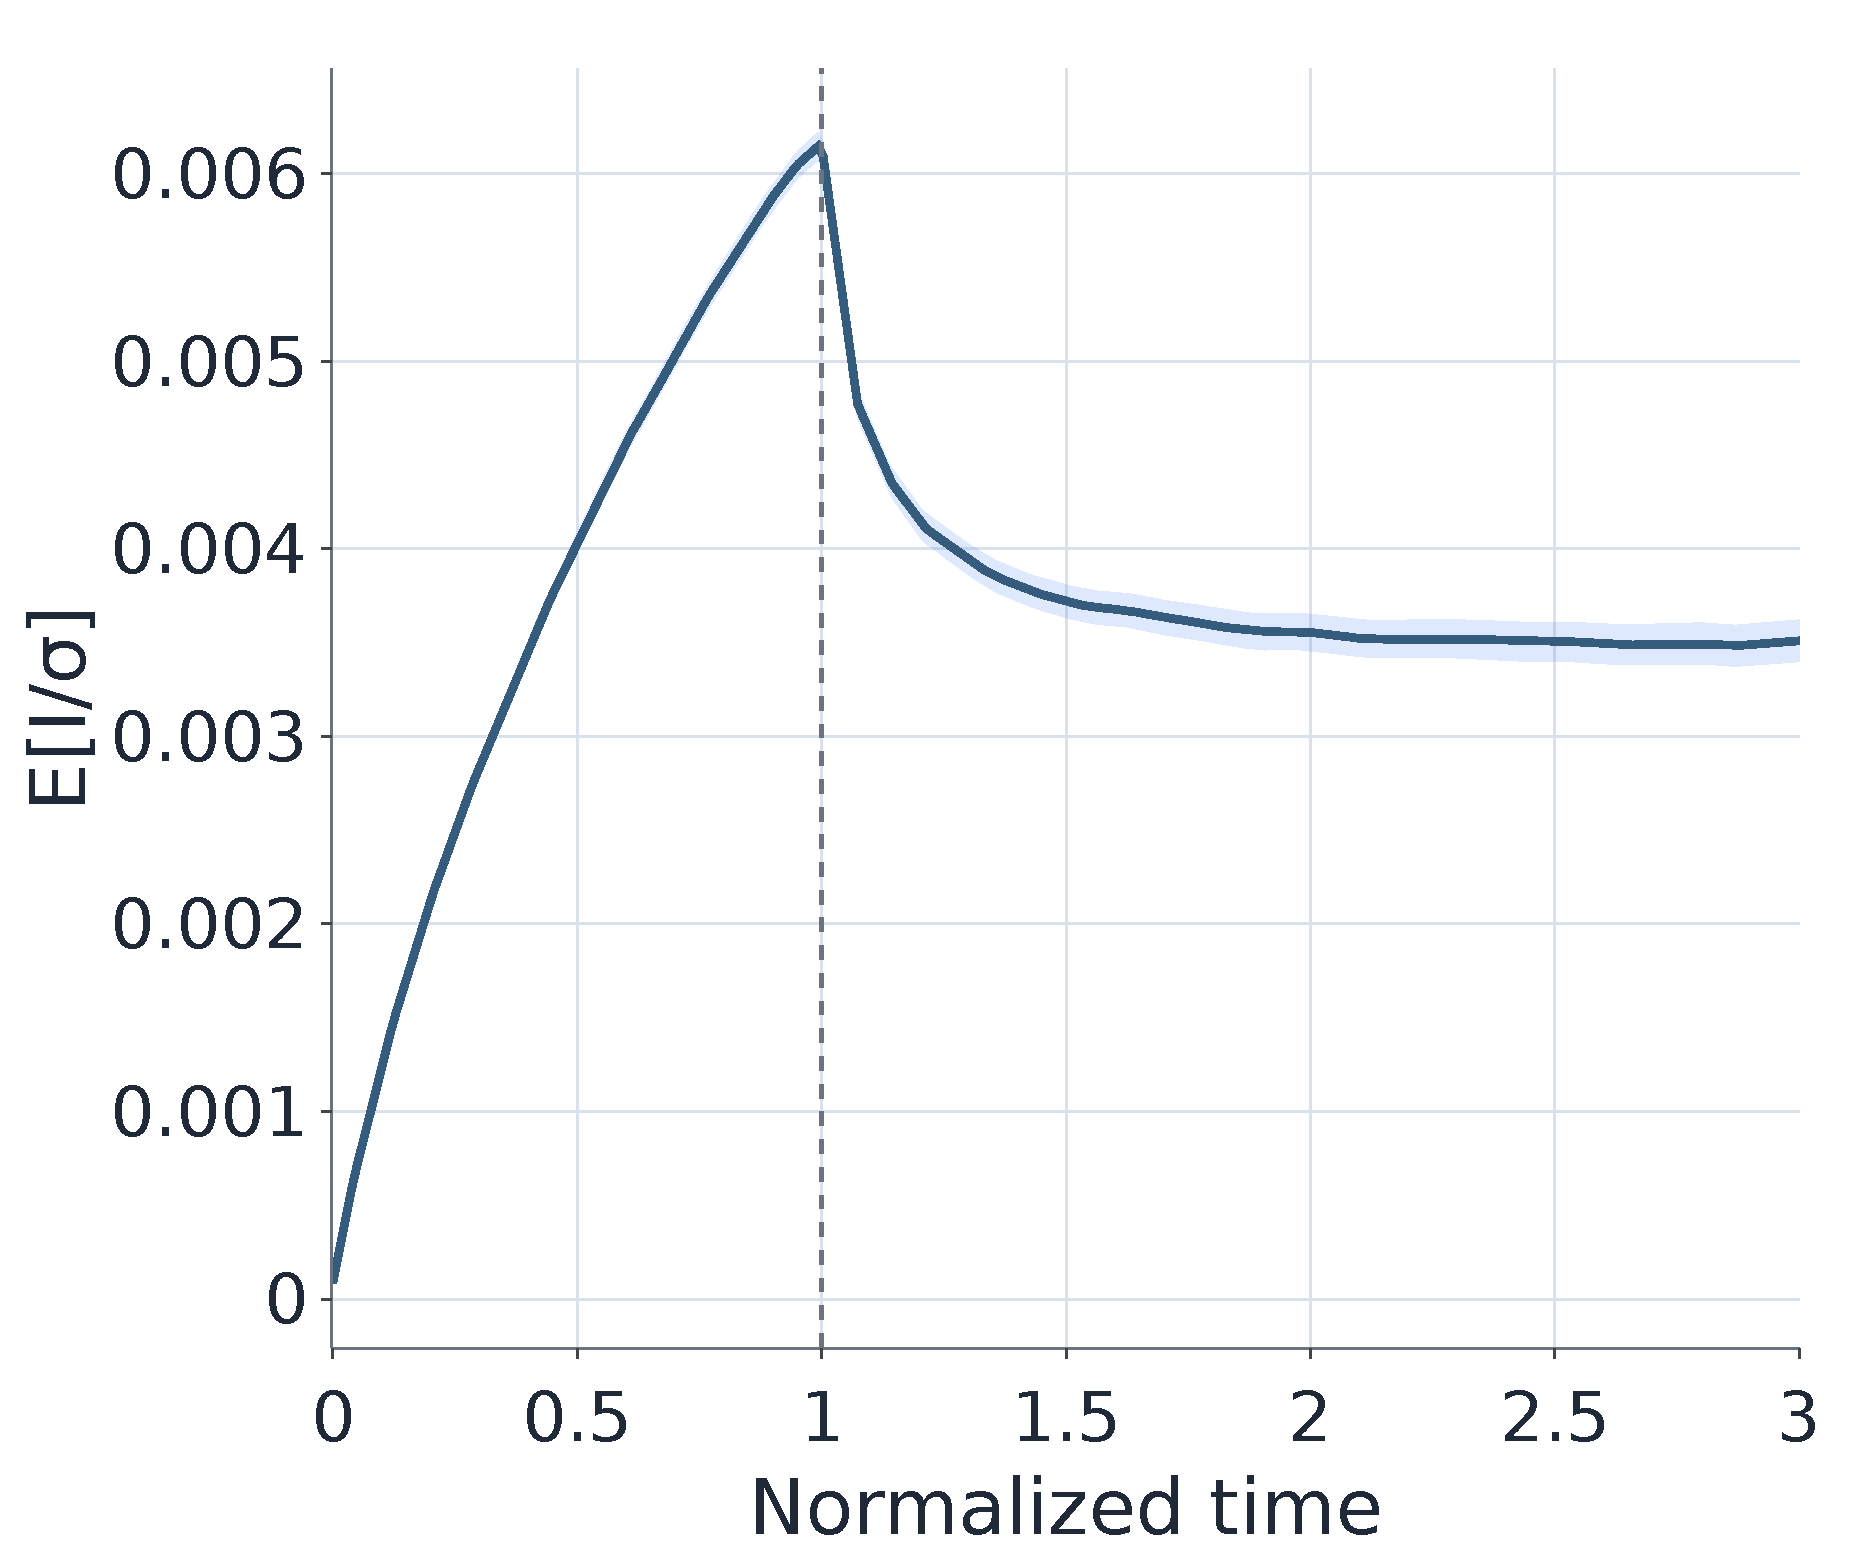
\includegraphics[width=\linewidth]{images/member_non_proprietary/png/normalized_impact_path_member_non_proprietary}
      \caption{Client}
    \end{subfigure}

  \end{adjustwidth}

  \caption{Mean normalised impact paths $\bar I_G(\tau)$. Time is normalised so that $\tau = 0$ at the start of the 
  metaorder and $\tau = 1$ at its end; the dashed line marks $\tau = 1$.
  Shaded regions are $\pm$SEM.}
  \label{fig:normalized_impact_paths}
\end{figure}

Finally, nationality-conditioned dynamic-impact paths are treated as robustness diagnostics rather than main estimates and are reported in Appendix~\ref{app:member_nationality_results}.

\FloatBarrier


\section{Crowding, Co-Impact, and the Proprietary Impact Premium}
\label{sec:crowding}

We now turn to crowding, namely the tendency of metaorders to align with
(or against) the contemporaneous net order flow of other metaorders.
Crowding is a key driver of co-impact and execution costs, since
metaorders that trade in the same direction as the rest of the market
face more adverse price pressure. This connects directly to the
institutional co-impact picture of \cite{BucciEtAl2020}.

All crowding measures in this section use the same notation. Let
\(\mathcal{G}=\{\mathrm{prop},\mathrm{client}\}\). For each instrument \(k\),
day \(d\), and group \(G\in\mathcal{G}\), let
\(\mathcal{M}_{k,d}^{G}\) be the set of reconstructed metaorders in group
\(G\) on that stock and date. Let
\(\mathcal{M}_{k,d}^{\mathrm{all}}
=\mathcal{M}_{k,d}^{\mathrm{prop}}\cup\mathcal{M}_{k,d}^{\mathrm{client}}\),
and let \(\bar G\) denote the other group (\(\bar{\mathrm{prop}}=\mathrm{client}\) and
\(\bar{\mathrm{client}}=\mathrm{prop}\)). For a target metaorder \(i\), write
\(k_i\), \(d_i\), and \(G_i\) for its instrument, date, and group.

For a target \(i\in\mathcal{M}_{k_i,d_i}^{G}\), we use three reference
environments,
\(R\in\{\mathrm{all},\mathrm{same},\mathrm{cross}\}\), defined by
\begin{equation}
  \mathcal{R}_i^{G,R} =
  \begin{cases}
    \mathcal{M}_{k_i,d_i}^{\mathrm{all}}\setminus\{i\},
      & R=\mathrm{all},\\
    \mathcal{M}_{k_i,d_i}^{G}\setminus\{i\},
      & R=\mathrm{same},\\
    \mathcal{M}_{k_i,d_i}^{\bar G},
      & R=\mathrm{cross}.
  \end{cases}
  \label{eq:crowding_reference_sets}
\end{equation}
We consider the volume-weighted imbalance is
\begin{equation}
  m_i^{G,R}
  =
  \frac{\displaystyle\sum_{j\in\mathcal{R}_i^{G,R}} Q_j\varepsilon_j}
       {\displaystyle\sum_{j\in\mathcal{R}_i^{G,R}} Q_j},
  \qquad i\in\mathcal{M}_{k_i,d_i}^{G}.
  \label{eq:crowding_imbalance}
\end{equation}
The statistic is left undefined when the denominator is zero. Positive values
mean that the reference environment of metaorder \(i\) is buy-dominated, while
negative values mean that it is sell-dominated.

We use the direction--imbalance correlation
\begin{equation}
  r^{G,R}
  =
  \mathrm{Corr}\!\left(\varepsilon_i,m_i^{G,R}\mid G_i=G\right),
  \qquad G\in\mathcal{G},\quad R\in\{\mathrm{all},\mathrm{same},\mathrm{cross}\}
  \label{eq:crowding_correlation}
\end{equation}
with its daily version as
\begin{equation}
  r_d^{G,R}
  =
  \mathrm{Corr}\!\left(\varepsilon_i,m_i^{G,R}\mid G_i=G,\ d_i=d\right).
  \label{eq:daily_crowding_correlation}
\end{equation}
% The second is the target-signed alignment
% \begin{equation}
%   a_i^{G,R} = \varepsilon_i m_i^{G,R}.
%   \label{eq:crowding_alignment}
% \end{equation}
% Positive \(a_i^{G,R}\) means that the target metaorder trades in the same
% direction as its reference environment.

Metaorders executed on the same trading day are not independent, as they
share market conditions and common shocks. To obtain dependence-aware
uncertainty, we construct confidence intervals via a Date-cluster
bootstrap: we resample trading days with replacement, recompute the
relevant statistic on the resampled panel, and report percentile
\(95\%\) confidence intervals.

\subsection{Crowding vs all others}
\label{subsec:all_vs_all_crowding}

The broadest reference environment is \(R=\mathrm{all}\), where the target
metaorder is compared with all other reconstructed metaorders in the same stock
and day, pooling proprietary and client flow. Averaging \(r_d^{G,\mathrm{all}}\)
over days, we obtain mean daily correlations:
\(\bar r_d^{\mathrm{prop},\mathrm{all}} = 0.041\) with 95\% CI
\([0.037, 0.046]\), and \(\bar r_d^{\mathrm{client},\mathrm{all}} = 0.113\)
with 95\% CI \([0.105, 0.119]\).
We observe that client flow shows a stronger alignment with the overall daily
imbalance than proprietary flow. This broad benchmark therefore already indicates
that client metaorders are more crowded when crowding is measured relative to the
aggregate same-stock metaorder environment. The time series of the three-day
rolling average of \(r_d^{G,\mathrm{all}}\) is reported in the top panel of
Figure~\ref{fig:crowding_rolling_timeseries}.

\subsection{Within-group and cross-group crowding}
\label{subsec:imbalance}

The same notation separates two more specific reference environments. For
\(R=\mathrm{same}\), the reference set contains only other metaorders from the
same group as the target. For \(R=\mathrm{cross}\), the reference set contains
metaorders from the other group on the same stock and date.

For within-group crowding, we compute \(r^{G,\mathrm{same}}\) and
\(r_d^{G,\mathrm{same}}\) using Equations~\eqref{eq:crowding_imbalance}--\eqref{eq:daily_crowding_correlation}.
Daily correlations are computed for days with at least 100 metaorders and are
averaged across stocks. The time series of the three-day rolling average of
\(r_d^{G,\mathrm{same}}\) is plotted for proprietary and client flows separately
in the middle panel of Figure~\ref{fig:crowding_rolling_timeseries}.

In our dataset, within-group orderflow imbalance statistics are:
\begin{itemize}
  \item Proprietary flow.
    \begin{itemize}
      \item Global correlation:
            \(r^{\mathrm{prop},\mathrm{same}} = 0.108\) with \(95\%\) CI
            \([0.102, 0.113]\), \(n = 588{,}334\) metaorders.
      \item Mean daily correlation:
            \(\bar r_d^{\mathrm{prop},\mathrm{same}} = 0.081\) with \(95\%\)
            CI \([0.077, 0.086]\) over \(251\) days.
    \end{itemize}

  \item Client flow.
    \begin{itemize}
      \item Global correlation:
            \(r^{\mathrm{client},\mathrm{same}} = 0.187\) with \(95\%\) CI
            \([0.180, 0.196]\), \(n = 255{,}535\) metaorders.
      \item Mean daily correlation:
            \(\bar r_d^{\mathrm{client},\mathrm{same}} = 0.169\) with \(95\%\)
            CI \([0.162, 0.177]\) over \(251\) days.
    \end{itemize}
\end{itemize}
Thus both client and proprietary metaorders tend to trade with the local daily
imbalance, although client metaorders show a significantly larger correlation.

For cross-group crowding, \(r_d^{\mathrm{prop},\mathrm{cross}}\) measures the
correlation between proprietary directions and the client imbalance, while
\(r_d^{\mathrm{client},\mathrm{cross}}\) measures the correlation between client
directions and the proprietary imbalance.

Empirically we find
\begin{itemize}
  \item Global correlations:
    \begin{itemize}
      \item \(r^{\mathrm{prop},\mathrm{cross}} = -0.023\) with \(95\%\) CI
            \([-0.028, -0.018]\).
      \item \(r^{\mathrm{client},\mathrm{cross}} = -0.016\) with \(95\%\) CI
            \([-0.025, -0.007]\).
    \end{itemize}
  \item Mean daily correlations, computed on days with \(n\ge 100\):
    \begin{itemize}
      \item \(\bar r_d^{\mathrm{prop},\mathrm{cross}} = -0.018\) with \(95\%\)
            CI \([-0.023, -0.014]\),
      \item \(\bar r_d^{\mathrm{client},\mathrm{cross}} = -0.003\) with \(95\%\)
            CI \([-0.010, 0.004]\).
    \end{itemize}
\end{itemize}

The \(\mathrm{prop},\mathrm{cross}\) daily correlation is slightly negative,
indicating a very mild tendency for proprietary flow to trade against the
imbalance produced by client flow, which is reminiscent of the way different
institutional styles interact in \cite{BucciEtAl2020}. The
\(\mathrm{client},\mathrm{cross}\) correlation is close to zero with a confidence
interval that includes zero, suggesting no clear alignment or anti-alignment of
client metaorders with the proprietary environment. The time series of the
three-day rolling average of these cross-group correlations is shown in the
bottom panel of Figure~\ref{fig:crowding_rolling_timeseries}.

\begin{figure}[p]
  \centering
  \begin{subfigure}{0.85\textwidth}
    \centering
    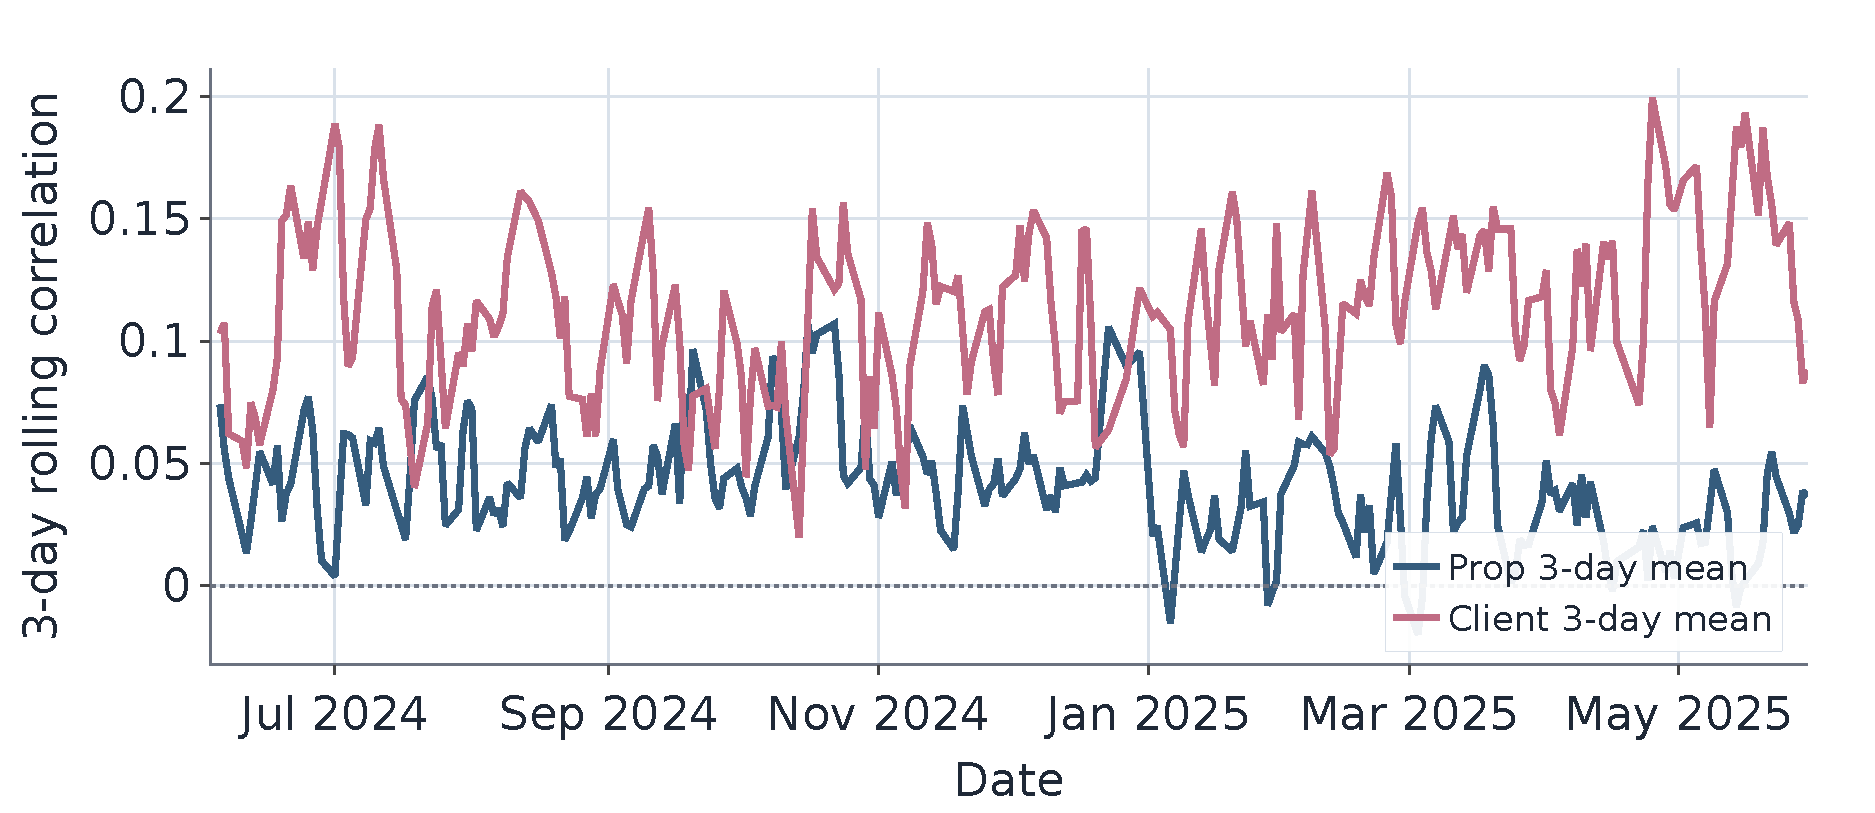
\includegraphics[width=\textwidth,height=0.22\textheight,keepaspectratio]{images/prop_vs_nonprop/png/all_vs_all_crowding_rolling_3d}
    \caption{All other metaorders, \(R=\mathrm{all}\).}
  \end{subfigure}
  \vspace{0.2em}
  \begin{subfigure}{0.85\textwidth}
    \centering
    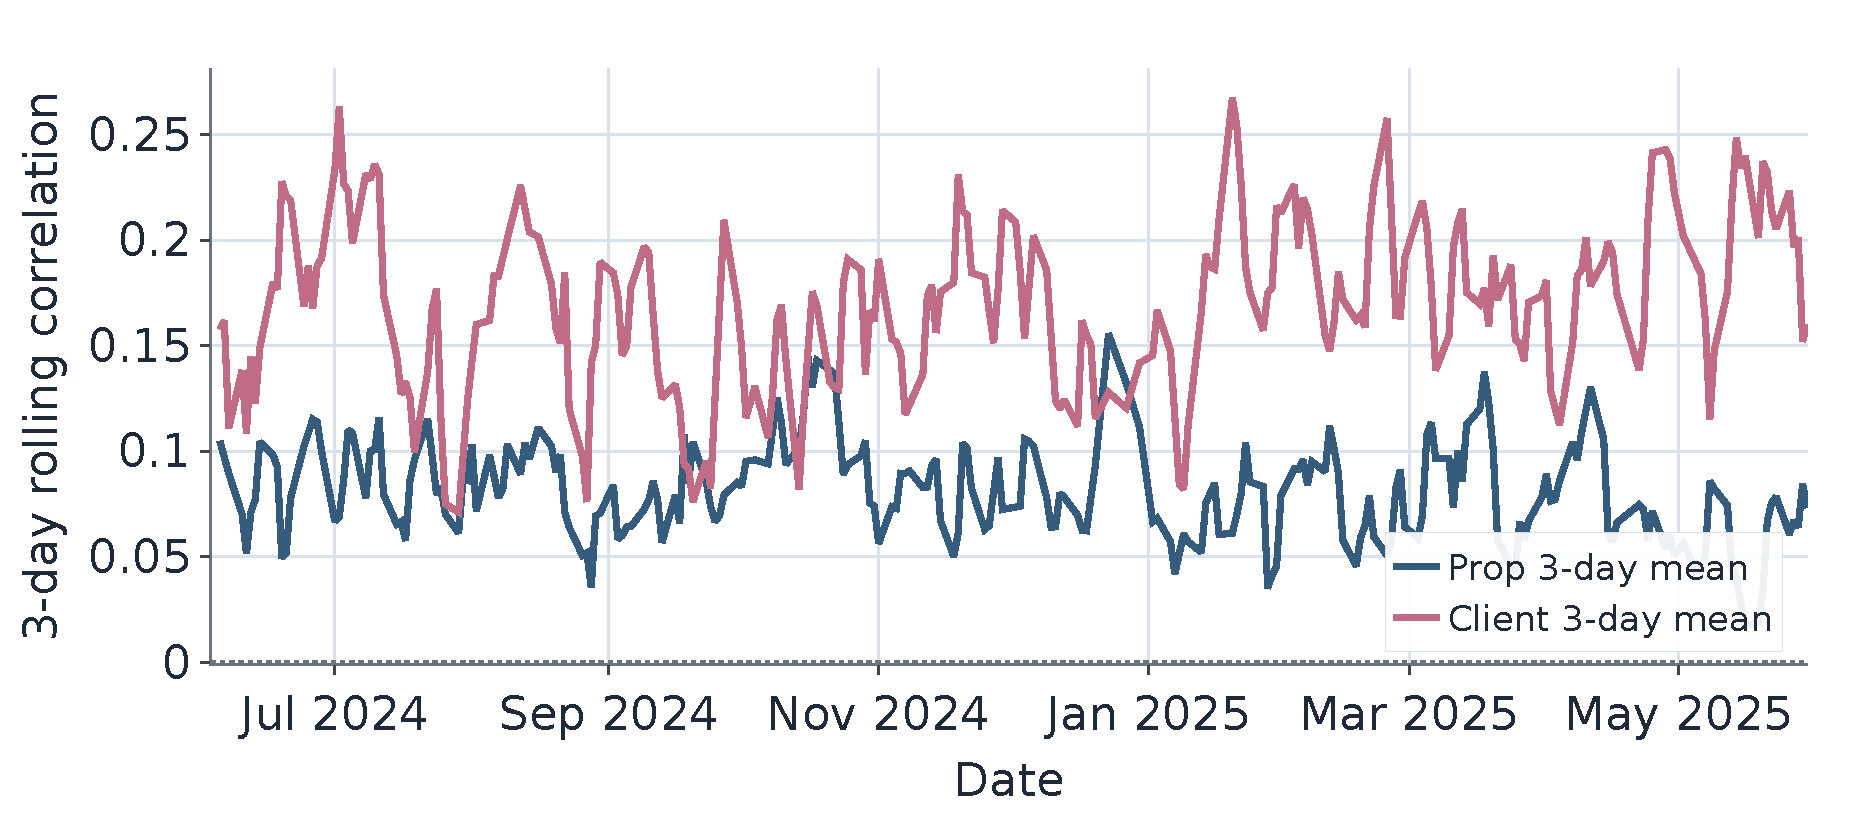
\includegraphics[width=\textwidth,height=0.22\textheight,keepaspectratio]{images/prop_vs_nonprop/png/daily_crowding_rolling_3d}
    \caption{Within-group imbalance, \(R=\mathrm{same}\).}
  \end{subfigure}
  \vspace{0.2em}
  \begin{subfigure}{0.85\textwidth}
    \centering
    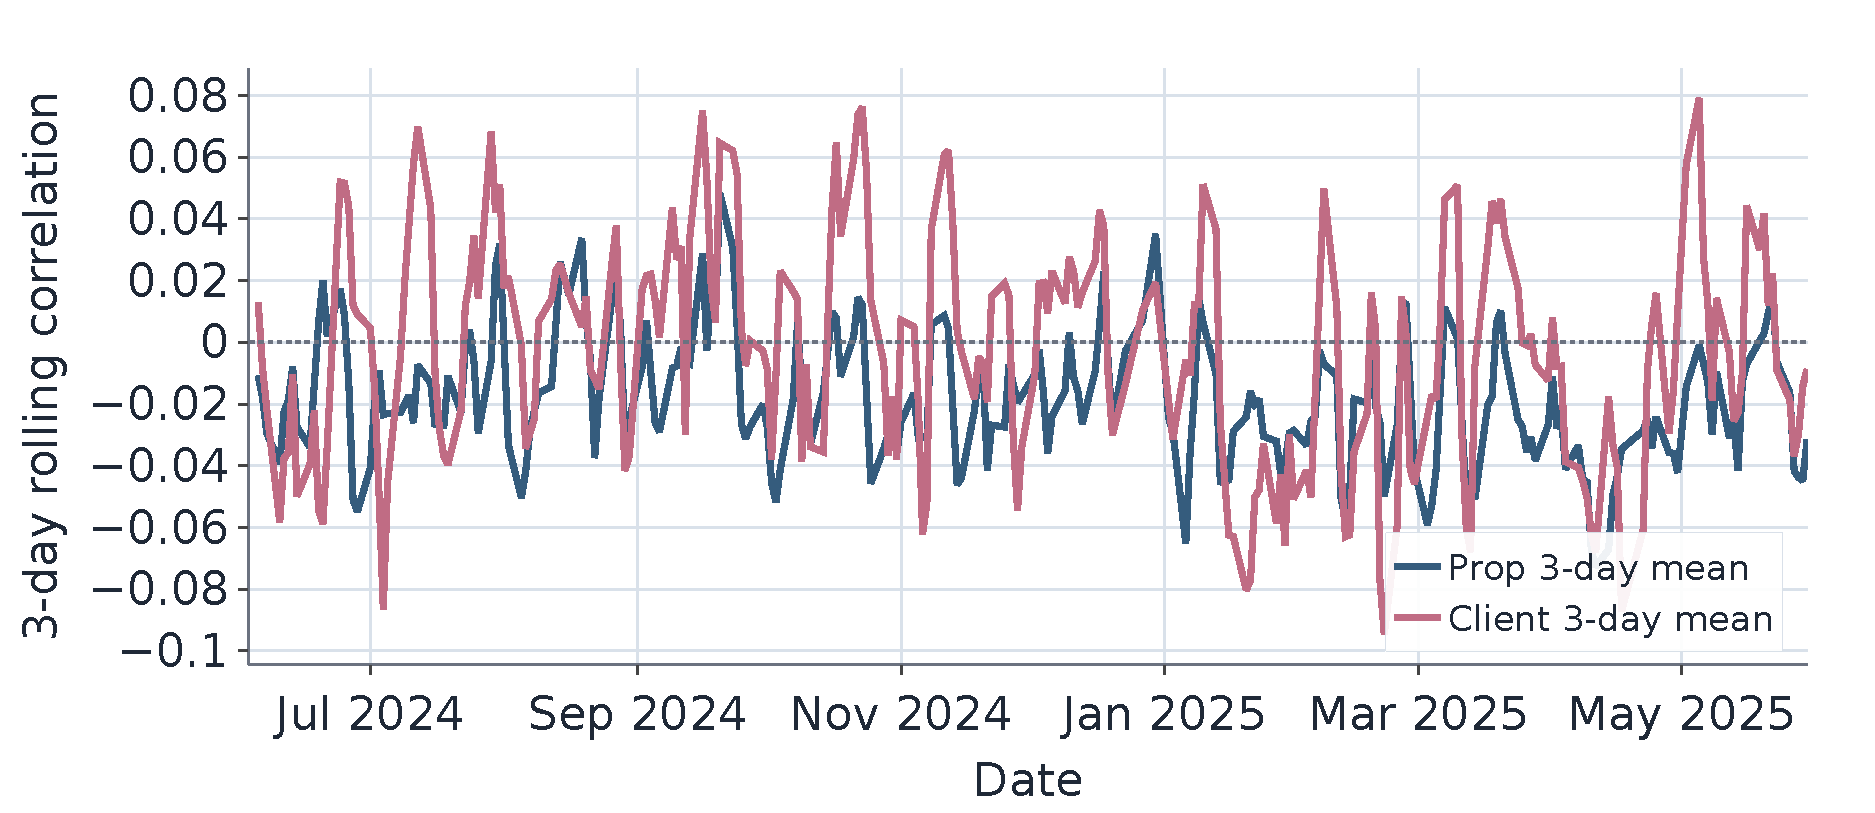
\includegraphics[width=\textwidth,height=0.22\textheight,keepaspectratio]{images/prop_vs_nonprop/png/cross_crowding_rolling_3d}
    \caption{Cross-group imbalance, \(R=\mathrm{cross}\).}
  \end{subfigure}
  \caption{Crowding rolling time series. Each panel reports the 3-day rolling
  mean of the relevant daily direction--imbalance correlation \(r_d^{G,R}\).
  Top: all other metaorders. Middle: within-group crowding. Bottom: cross-group
  crowding.}
  \label{fig:crowding_rolling_timeseries}
\end{figure}

\subsection{Crowding conditioned on participation rate}
\label{subsec:crowding_eta}

The previously defined execution participation rate \(\eta_i\) measures the
fraction of contemporaneous traded volume absorbed during the metaorder's own
execution window. We use \(\eta_i\) as an execution-state variable and ask
whether crowding becomes stronger at higher participation.

For each target group \(G\in\mathcal{G}\), we partition metaorders into deciles
of \(\eta_i\) using pooled quantiles, with common bin edges across groups. We
compute participation-conditioned statistics separately for
\(R\in\{\mathrm{same},\mathrm{cross}\}\). Within participation-rate bin \(b\),
we consider
\begin{align}
  A_b^{G,R}
  & = \E\!\left[\varepsilon_i m_i^{G,R}\mid G_i=G,\ \eta_i\in b\right],
  \\
  U_b^{G,R}
  &= \E\!\left[|m_i^{G,R}|\mid G_i=G,\ \eta_i\in b\right].
\end{align}
The statistic \(A_b^{G,R}\) measures signed alignment with the reference
environment, while \(U_b^{G,R}\) measures how one-sided that environment is,
independently of target direction. Confidence bands are obtained via a block
bootstrap that resamples trading days with replacement (1000 replicates), which
accounts for cross-sectional dependence within the same date.

\paragraph{Within-group conditioning.}
Figure~\ref{fig:crowding_vs_eta_local} shows that both groups become more
crowded as \(\eta\) increases. The effect is monotone and much stronger for
client flow: high-participation client metaorders are strongly aligned with the
contemporaneous within-client imbalance, while low-\(\eta\) metaorders are close
to neutral. Proprietary flow exhibits a milder but statistically significant
increase. In addition, \(U_b^{G,\mathrm{same}}\) increases with \(\eta\) for both
groups, indicating that high-participation executions tend to occur on \((k,d)\)
pairs where the rest of the same-group flow is more one-sided.

\paragraph{Cross-group conditioning.}
Figure~\ref{fig:crowding_vs_eta_cross} reveals a different pattern across
groups. While the magnitude of the other group's imbalance increases with
\(\eta\) for both proprietary and client metaorders, the alignment statistics
diverge. Proprietary metaorders are weakly contrarian to the client environment
across \(\eta\) with no pronounced trend, whereas client metaorders become
increasingly contrarian to the proprietary environment at high \(\eta\). This
behaviour is consistent with an intermediation/risk-transfer picture in which
aggressive client demand is partly offset by proprietary flow.

\begin{figure}[p]
  \centering
  \begin{subfigure}{0.70\textwidth}
    \centering
    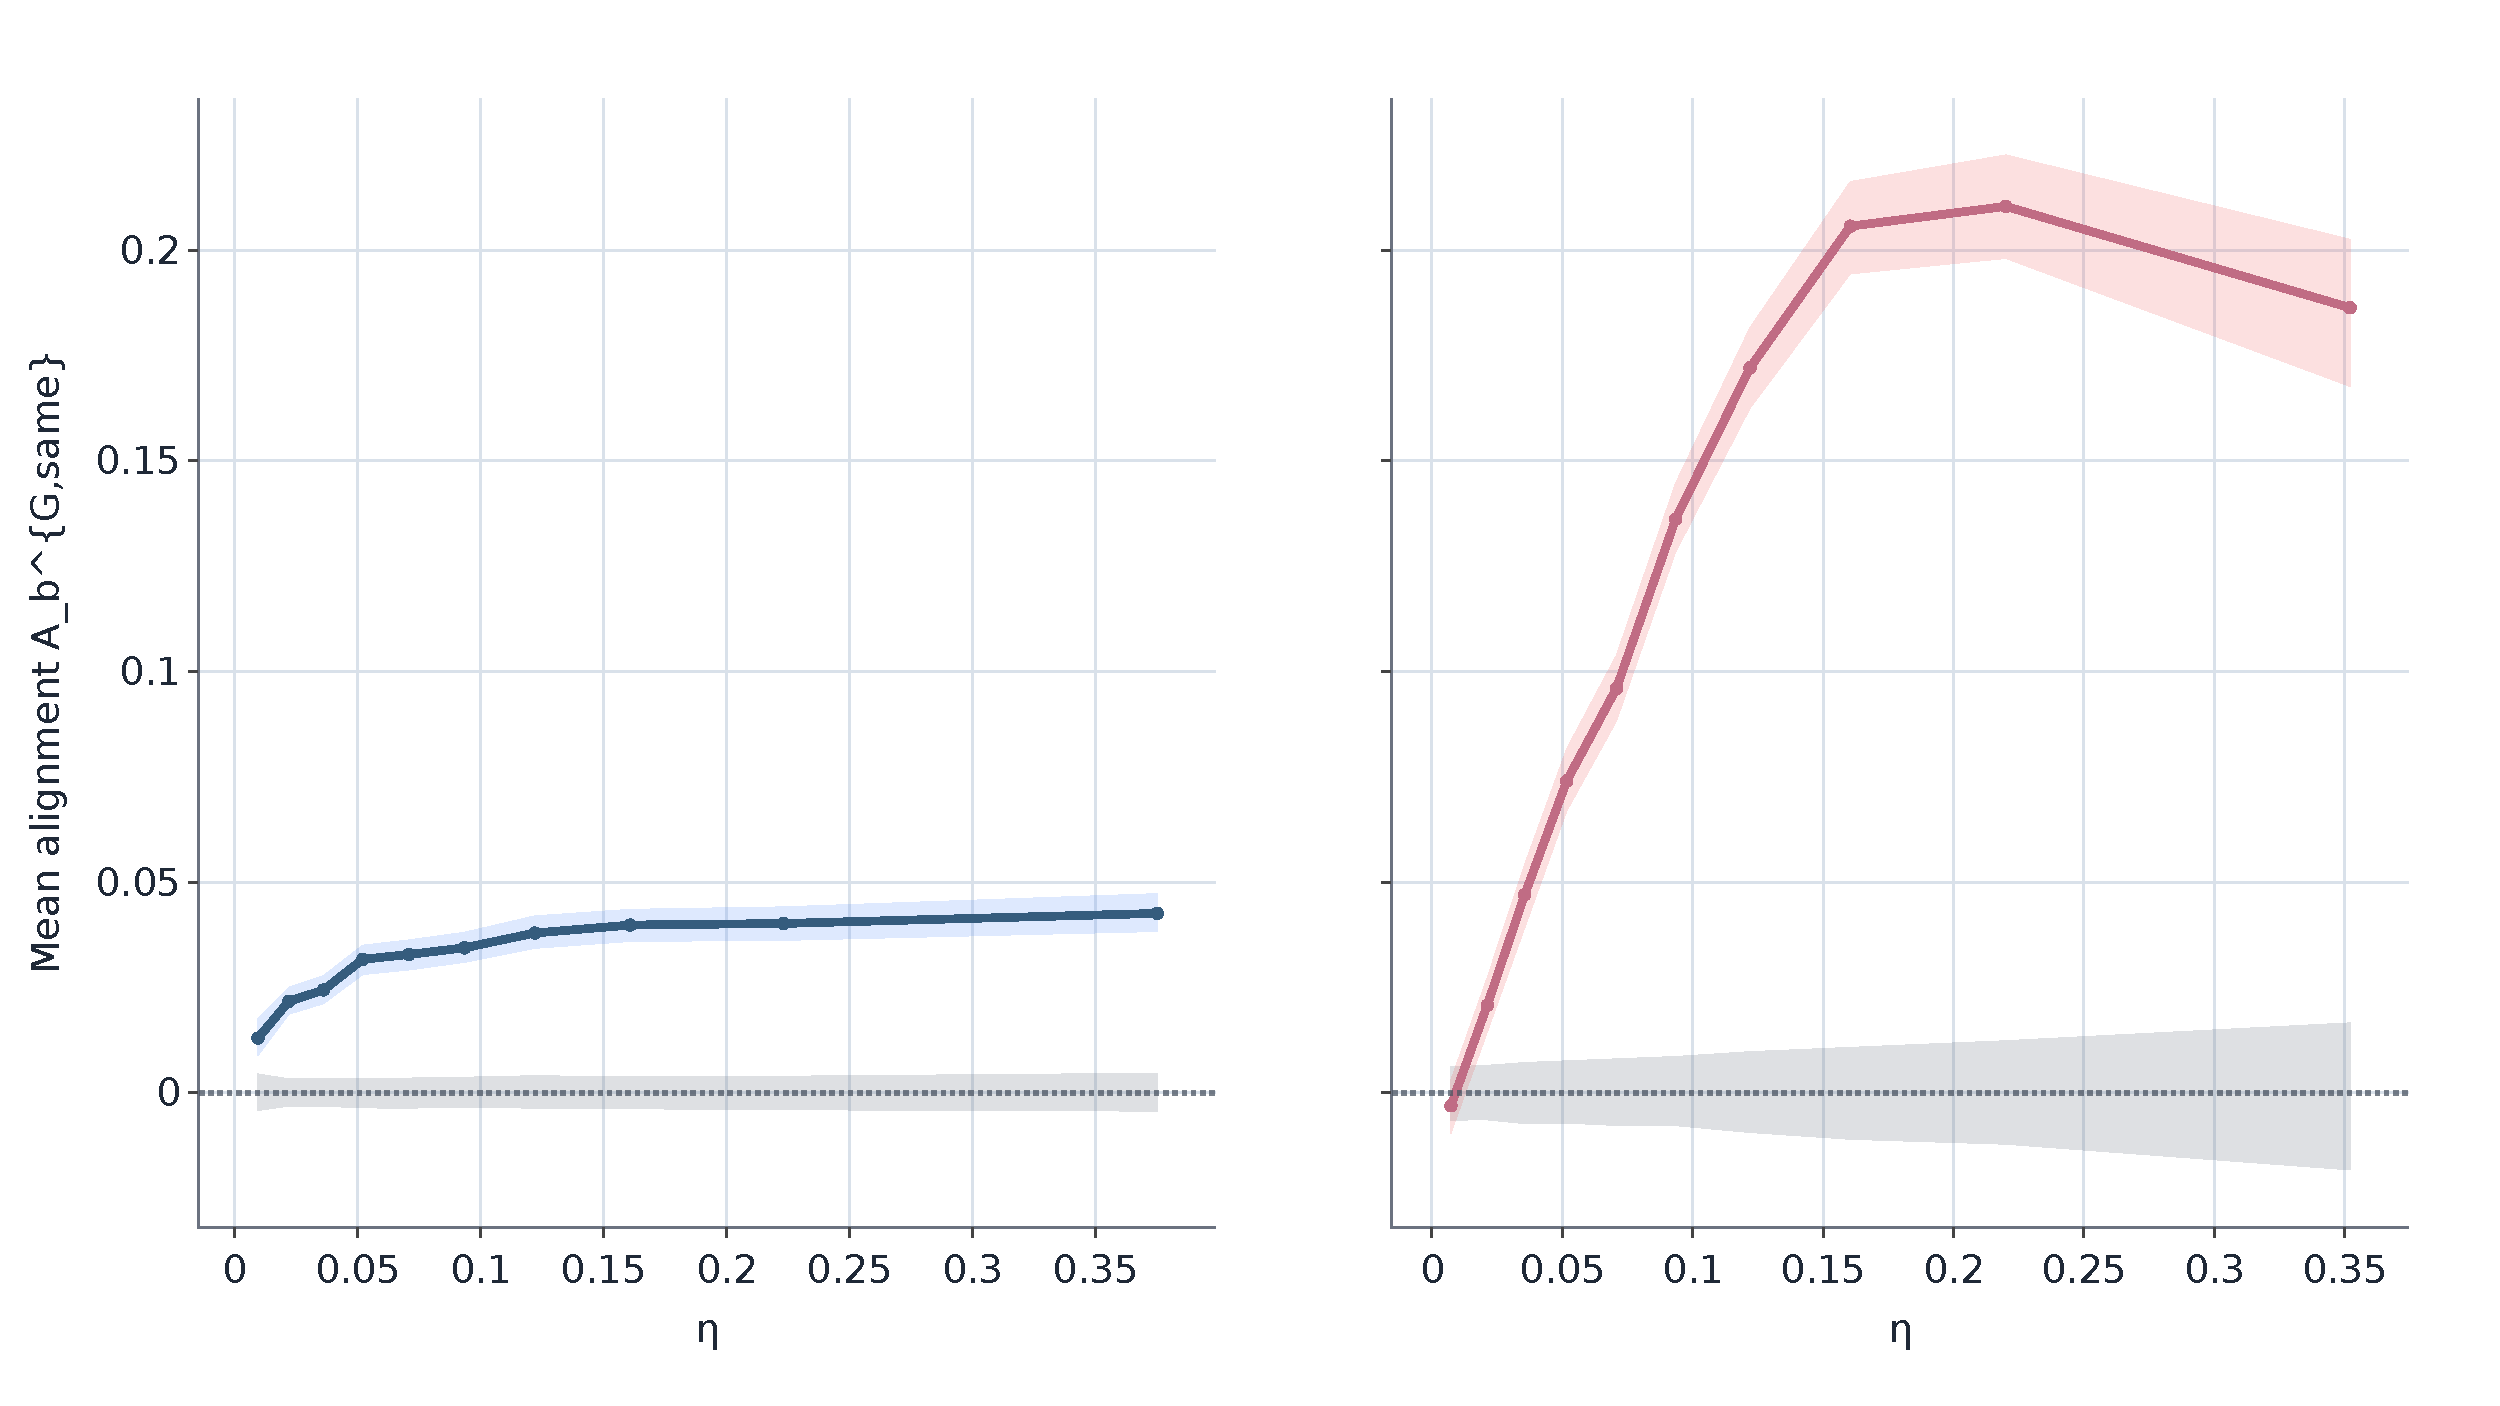
\includegraphics[width=\linewidth]{images/crowding_vs_part_rate/png/curve_mean_align_vs_eta_local}
    \caption{Mean alignment \(A_b^{G,\mathrm{same}} = \E[a_i^{G,\mathrm{same}}\mid \eta_i\in b]\).}
  \end{subfigure}

  \vspace{0.8em}

  \begin{subfigure}{0.70\textwidth}
    \centering
    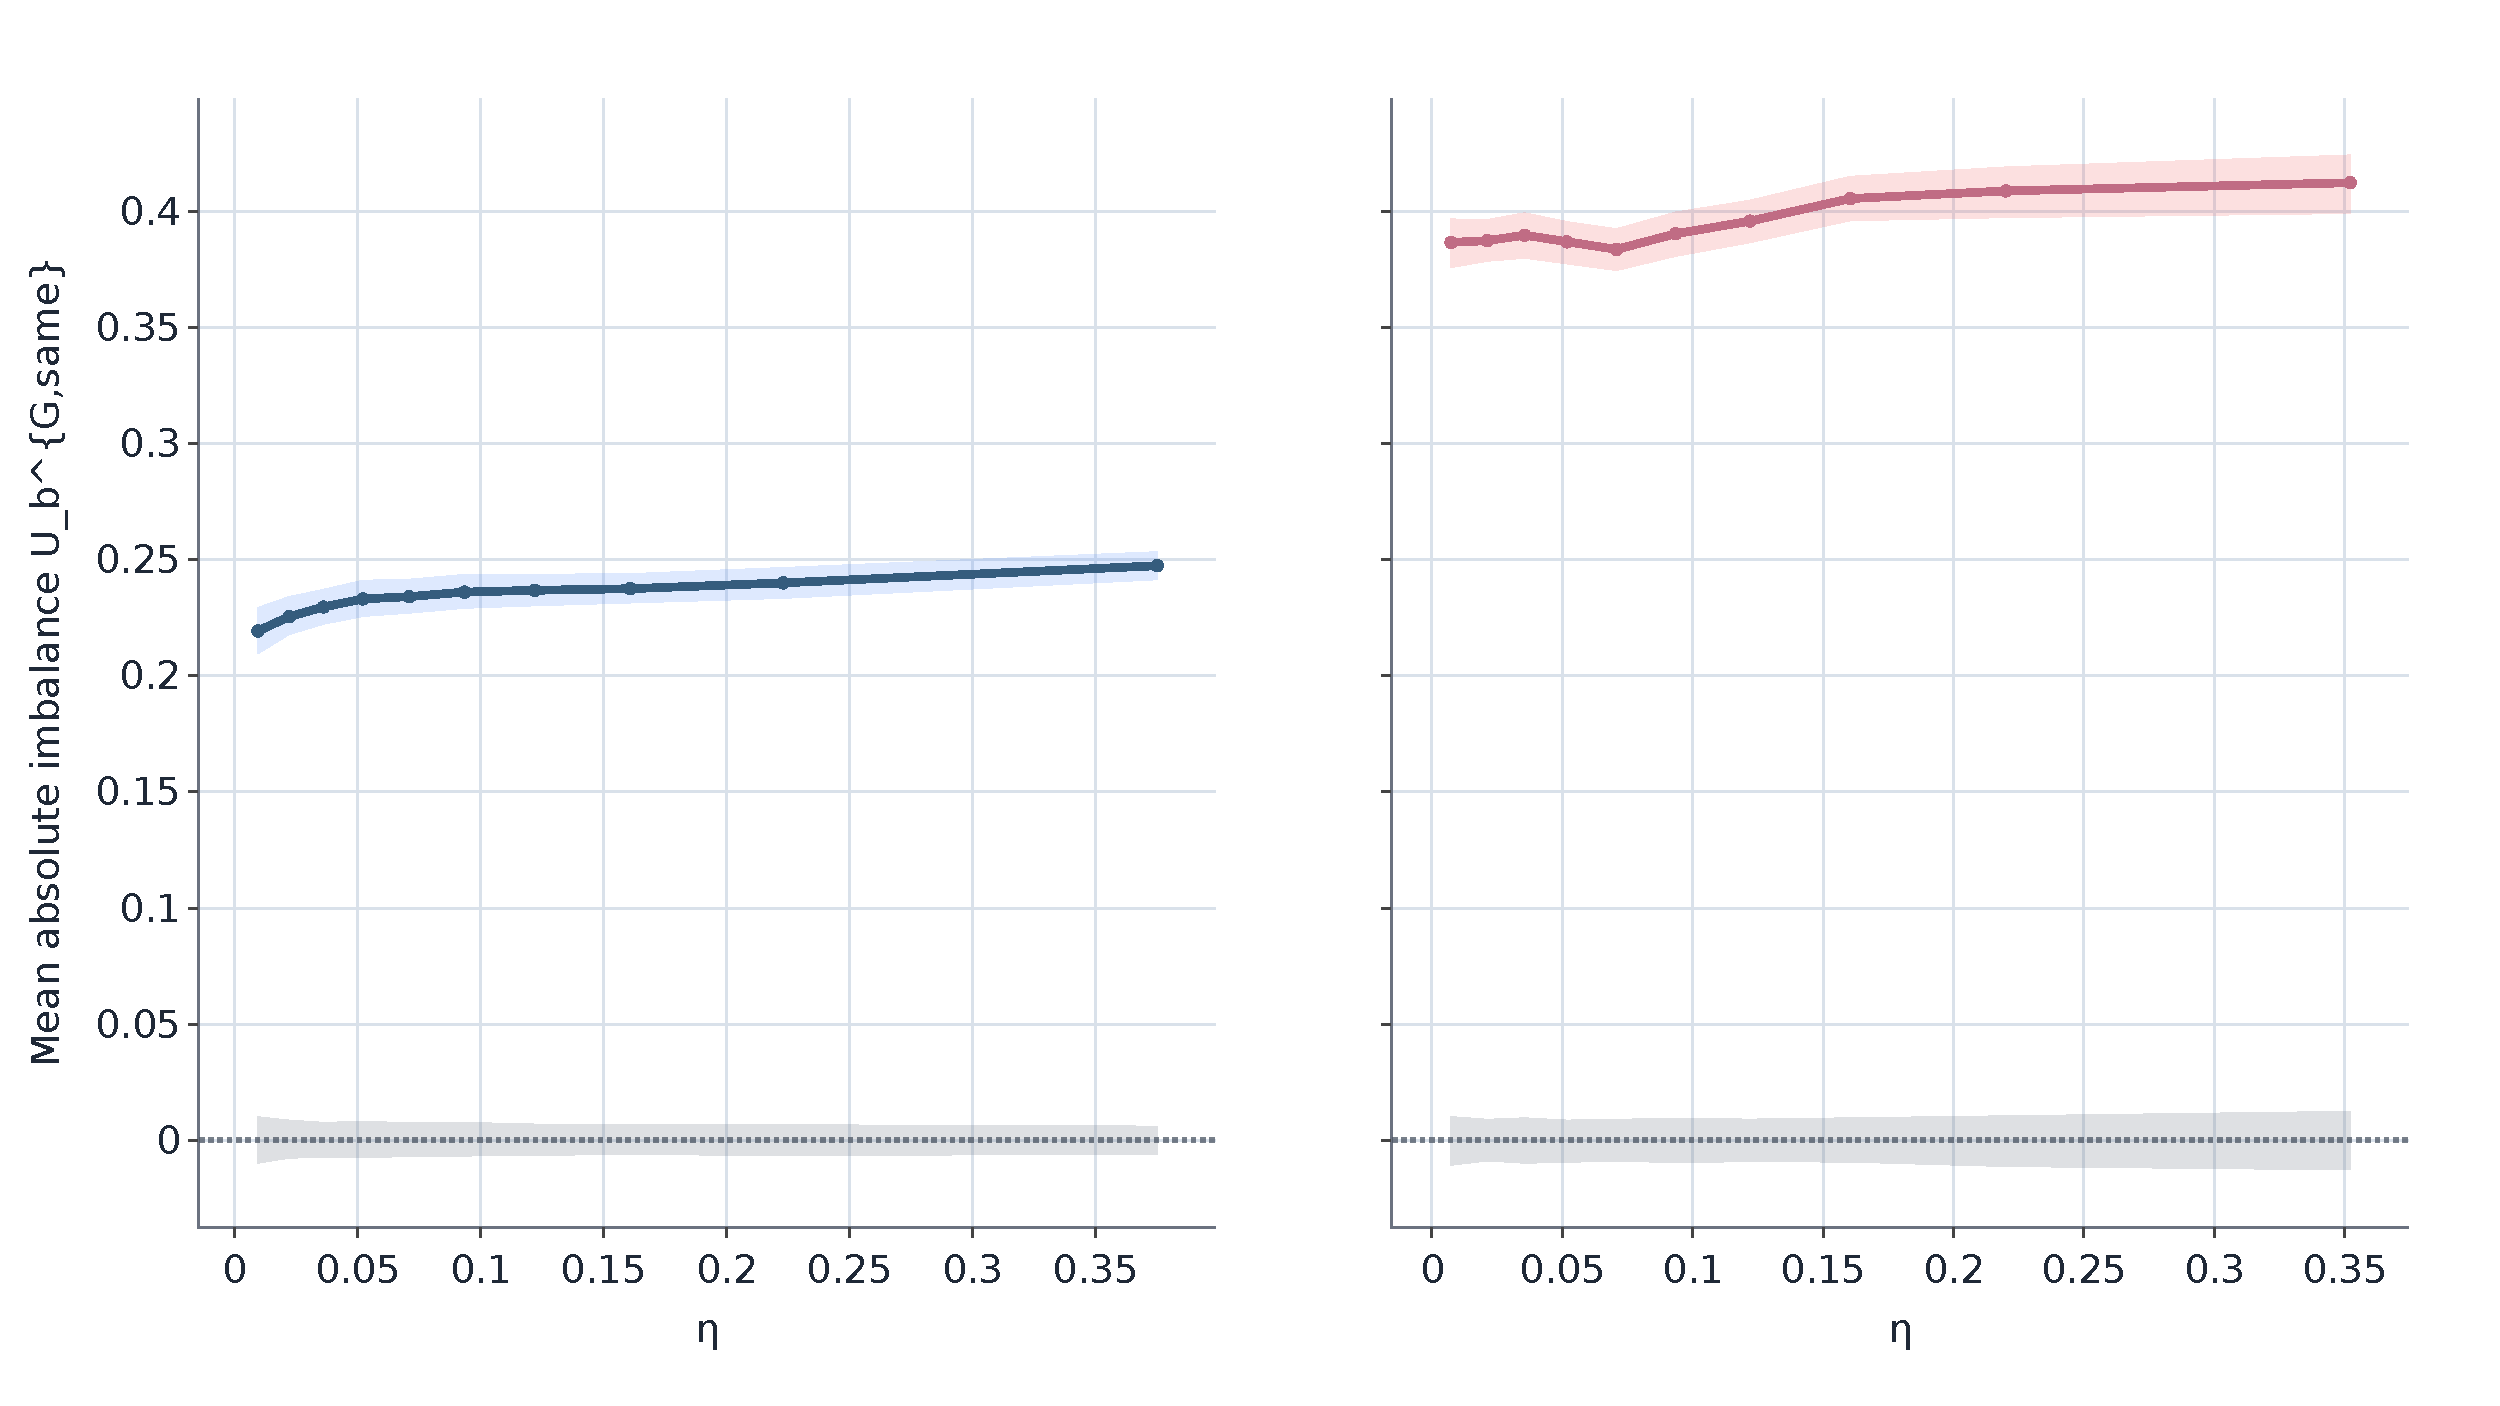
\includegraphics[width=\linewidth]{images/crowding_vs_part_rate/png/curve_mean_abs_imb_vs_eta_local}
    \caption{Mean absolute imbalance \(U_b^{G,\mathrm{same}} = \E[|m_i^{G,\mathrm{same}}|\mid \eta_i\in b]\).}
  \end{subfigure}
  \caption{Within-group crowding conditioned on participation-rate deciles. Each
  plot has two panels (left: proprietary, right: client). Shaded regions are
  95\% day-cluster bootstrap confidence bands.}
  \label{fig:crowding_vs_eta_local}
\end{figure}

\begin{figure}[p]
  \centering
  \begin{subfigure}{0.70\textwidth}
    \centering
    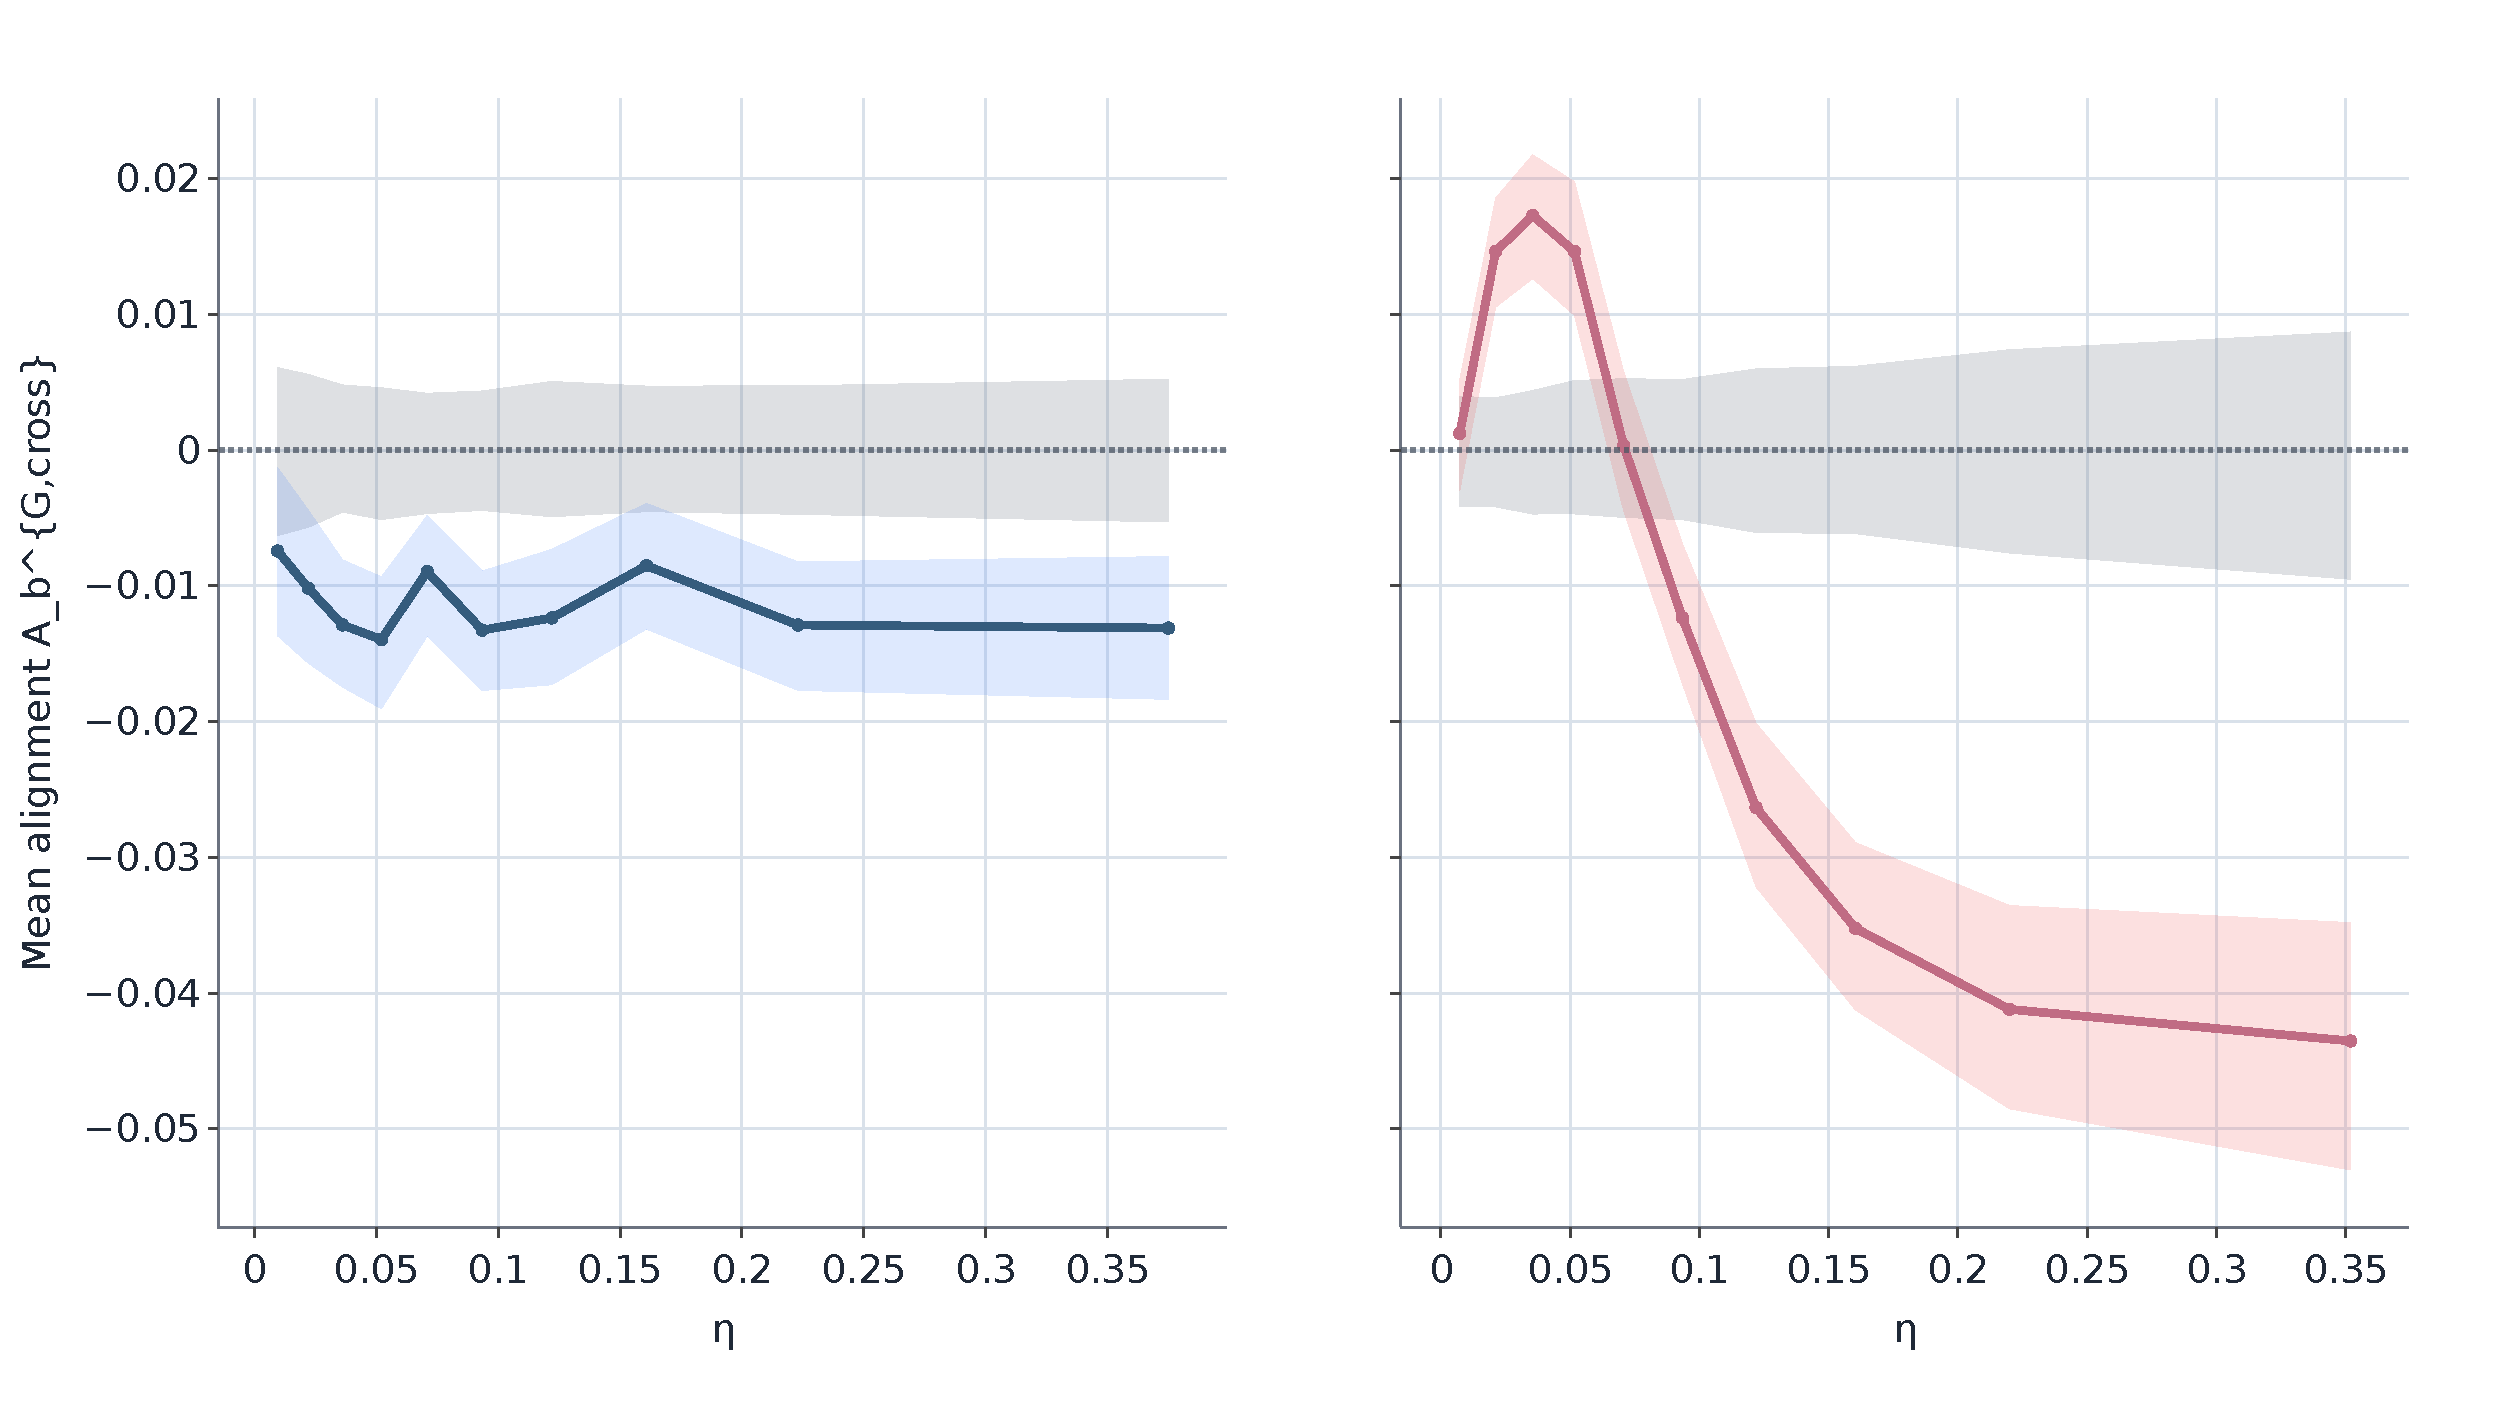
\includegraphics[width=\linewidth]{images/crowding_vs_part_rate/png/curve_mean_align_vs_eta_cross}
    \caption{Mean alignment \(A_b^{G,\mathrm{cross}} = \E[a_i^{G,\mathrm{cross}}\mid \eta_i\in b]\).}
  \end{subfigure}

  \vspace{0.8em}

  \begin{subfigure}{0.70\textwidth}
    \centering
    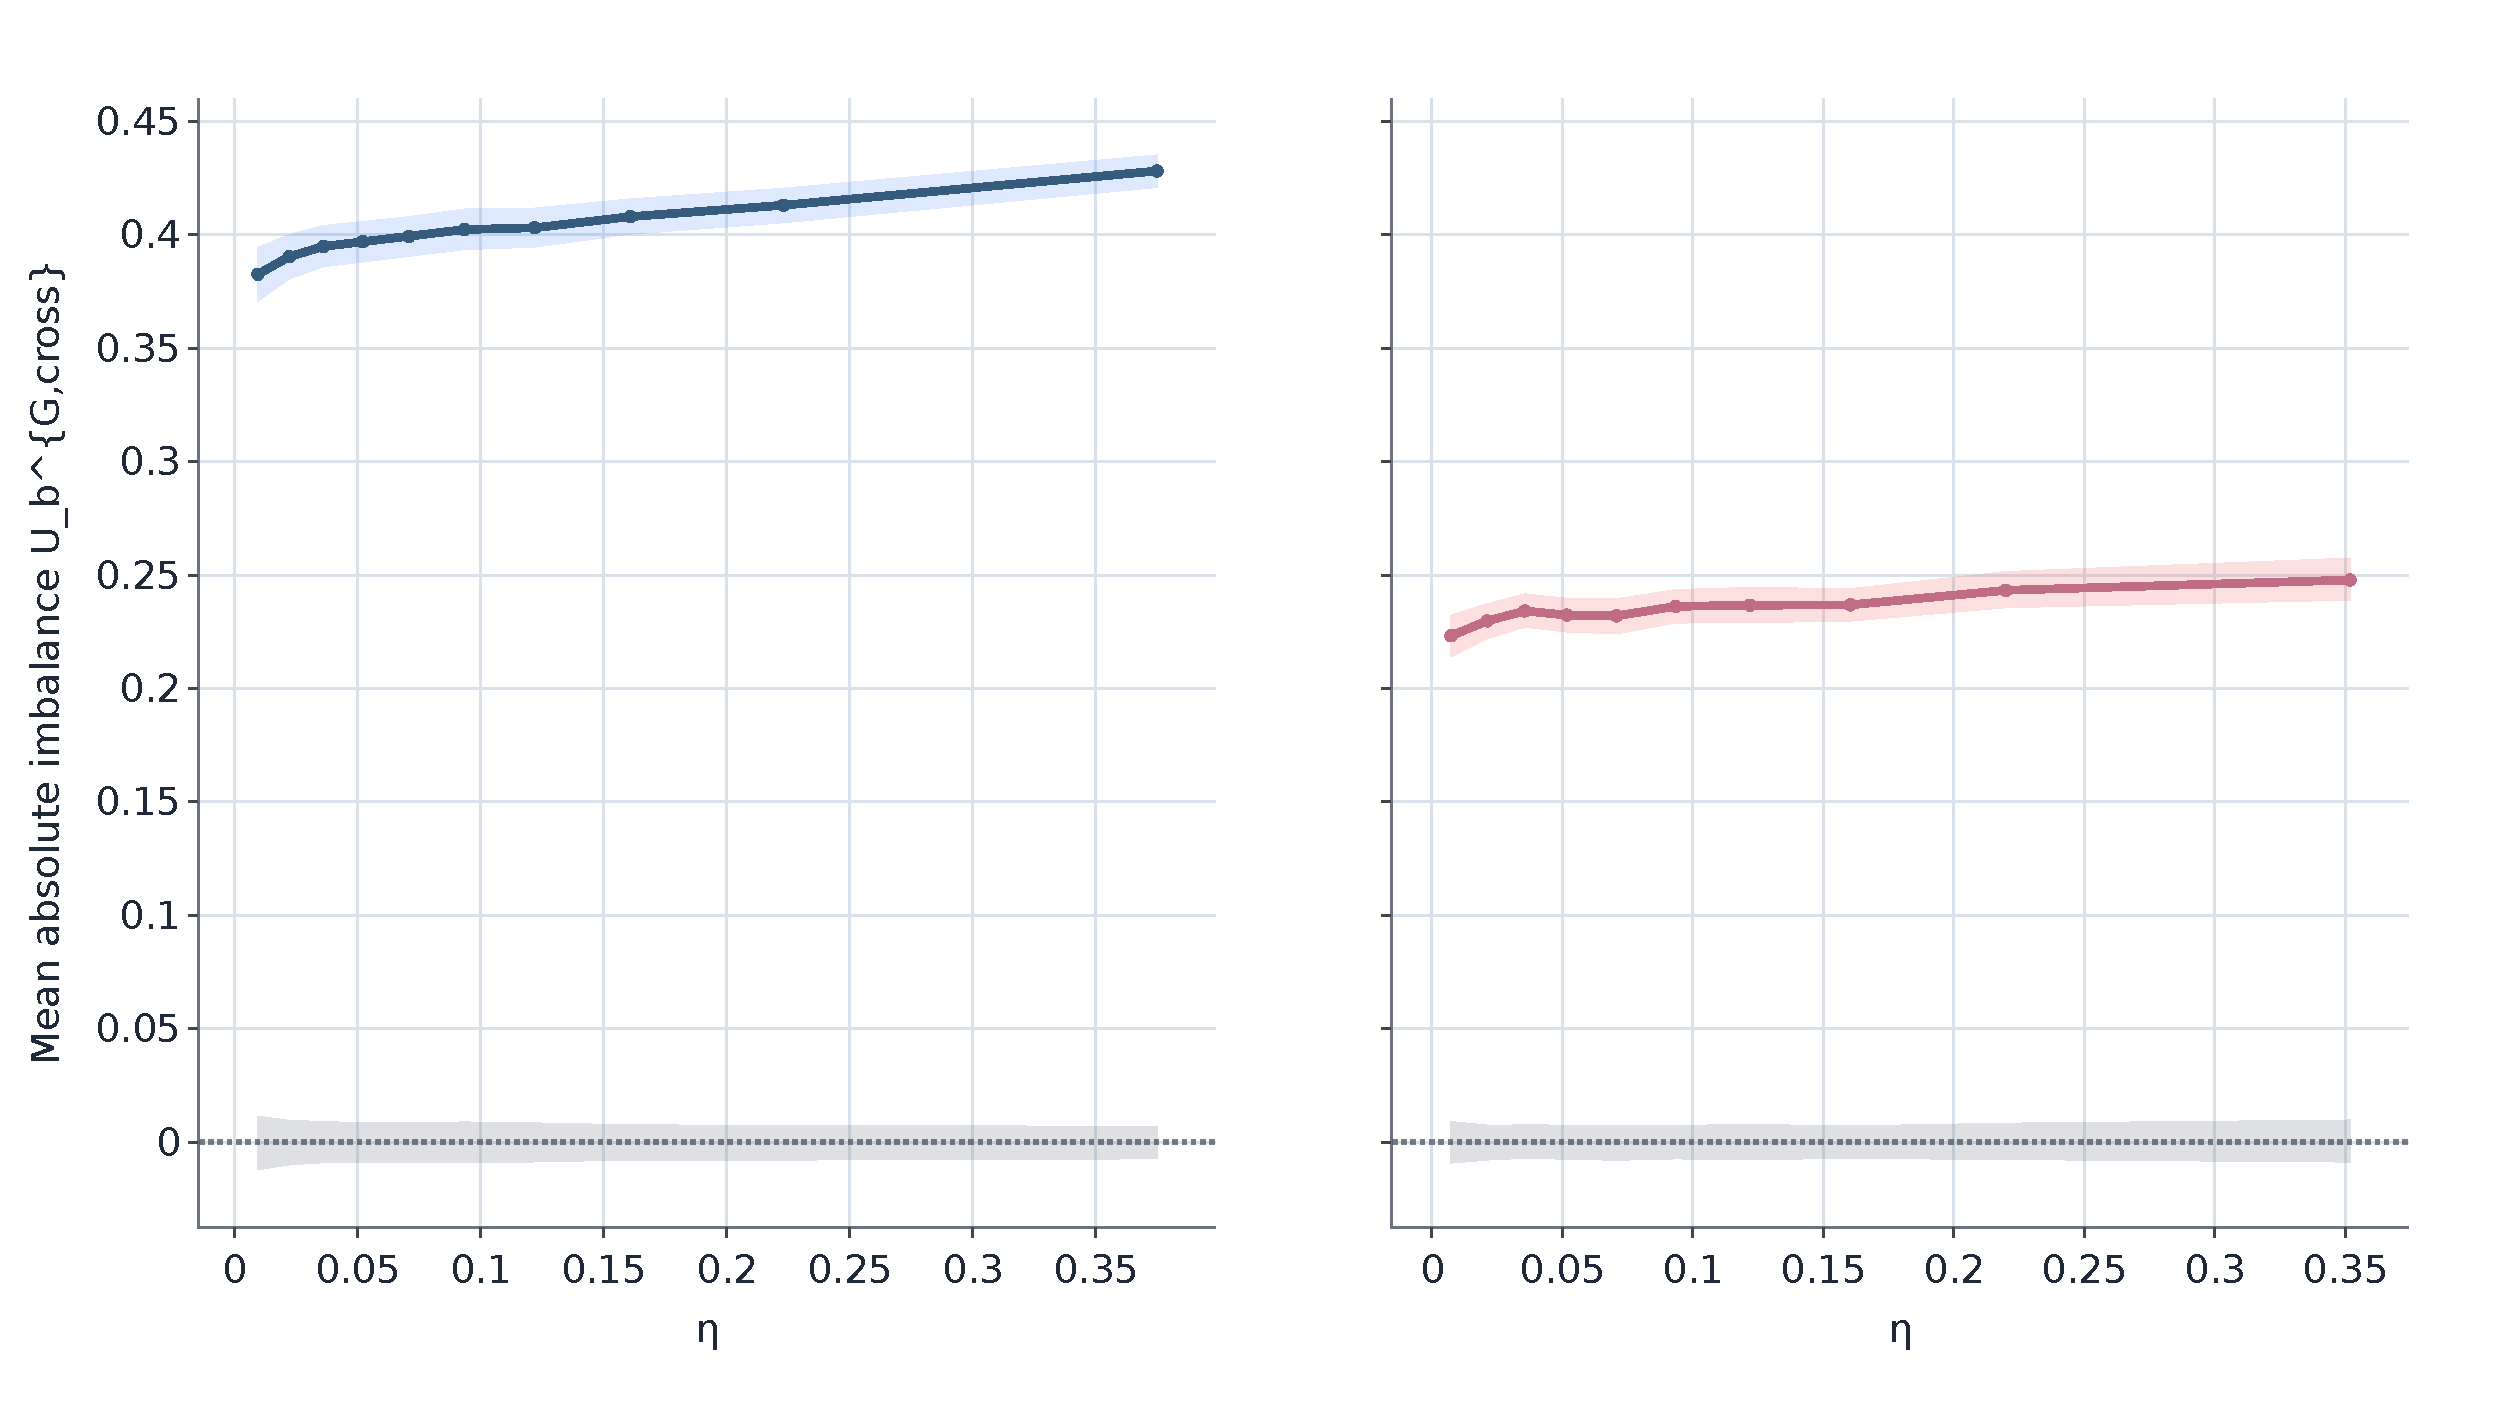
\includegraphics[width=\linewidth]{images/crowding_vs_part_rate/png/curve_mean_abs_imb_vs_eta_cross}
    \caption{Mean absolute imbalance \(U_b^{G,\mathrm{cross}} = \E[|m_i^{G,\mathrm{cross}}|\mid \eta_i\in b]\).}
  \end{subfigure}
  \caption{Cross-group crowding conditioned on participation-rate deciles. The
  imbalance \(m_i^{G,\mathrm{cross}}\) is constructed from the other group on the
  same \((k,d)\). Each plot has two panels (left: proprietary, right: client);
  shaded regions are 95\% day-cluster bootstrap confidence bands.}
  \label{fig:crowding_vs_eta_cross}
\end{figure}

\subsection{Does crowding explain the higher impact of proprietary flow?}
\label{subsec:crowding_impact}

The previous subsections show that crowding is economically meaningful for both
groups and, when measured at the daily stock level, often stronger for client
flow. We now return to the question raised by the impact curves in
Section~\ref{subsec:impact_models}: why do proprietary metaorders have larger
impact over the empirically relevant range of \(Q/V\)? This subsection asks,
step by step, whether crowding helps explain the source of the impact
difference.

We first use the all-flow reference environment, \(R=\mathrm{all}\). For each
target metaorder, define
\begin{equation}
  a_i^{\mathrm{all}} \equiv a_i^{G_i,\mathrm{all}}
  = \varepsilon_i m_i^{G_i,\mathrm{all}}.
\end{equation}
Positive \(a_i^{\mathrm{all}}\) means that metaorder \(i\) trades in the same
direction as the aggregate same-stock same-day imbalance generated by all other
metaorders.

We then sort proprietary and client metaorders separately into terciles of
\(a_i^{\mathrm{all}}\) and re-estimate the standard power-law model for the
normalized signed impact \(I_i\), defined in Equation~\eqref{impact_def}, within
each tercile. Table~\ref{tab:crowding_impact_terciles} reports the difference
between fitted impact in the highest and lowest crowding terciles at two
benchmark sizes, while Figure~\ref{fig:impact_curves_by_crowding} shows the
overall curves. The difference is positive for both groups: metaorders that
trade with the same-day imbalance have larger fitted impact. The effect,
however, is larger and statistically significant for client flow, as shown in
the last row of Table~\ref{tab:crowding_impact_terciles}. These results add to
the previous message: proprietary metaorders are less crowded on average, and
their fitted impact is also less sensitive to this daily crowding variable.

However, because all-flow alignment and participation rate are themselves
positively related, especially for clients, Figure~\ref{fig:impact_curves_by_crowding_and_eta}
repeats the comparison conditioned on two levels of \(\eta\), smaller and larger
than the median \footnote{In the Client / low $\eta$ panel, there are no 
enough data points for the intermediate terciles}. The crowding premium remains visible, but becomes more
heterogeneous, indicating that crowding and execution aggressiveness interact
rather than entering independently.

\begin{figure}
  \centering
  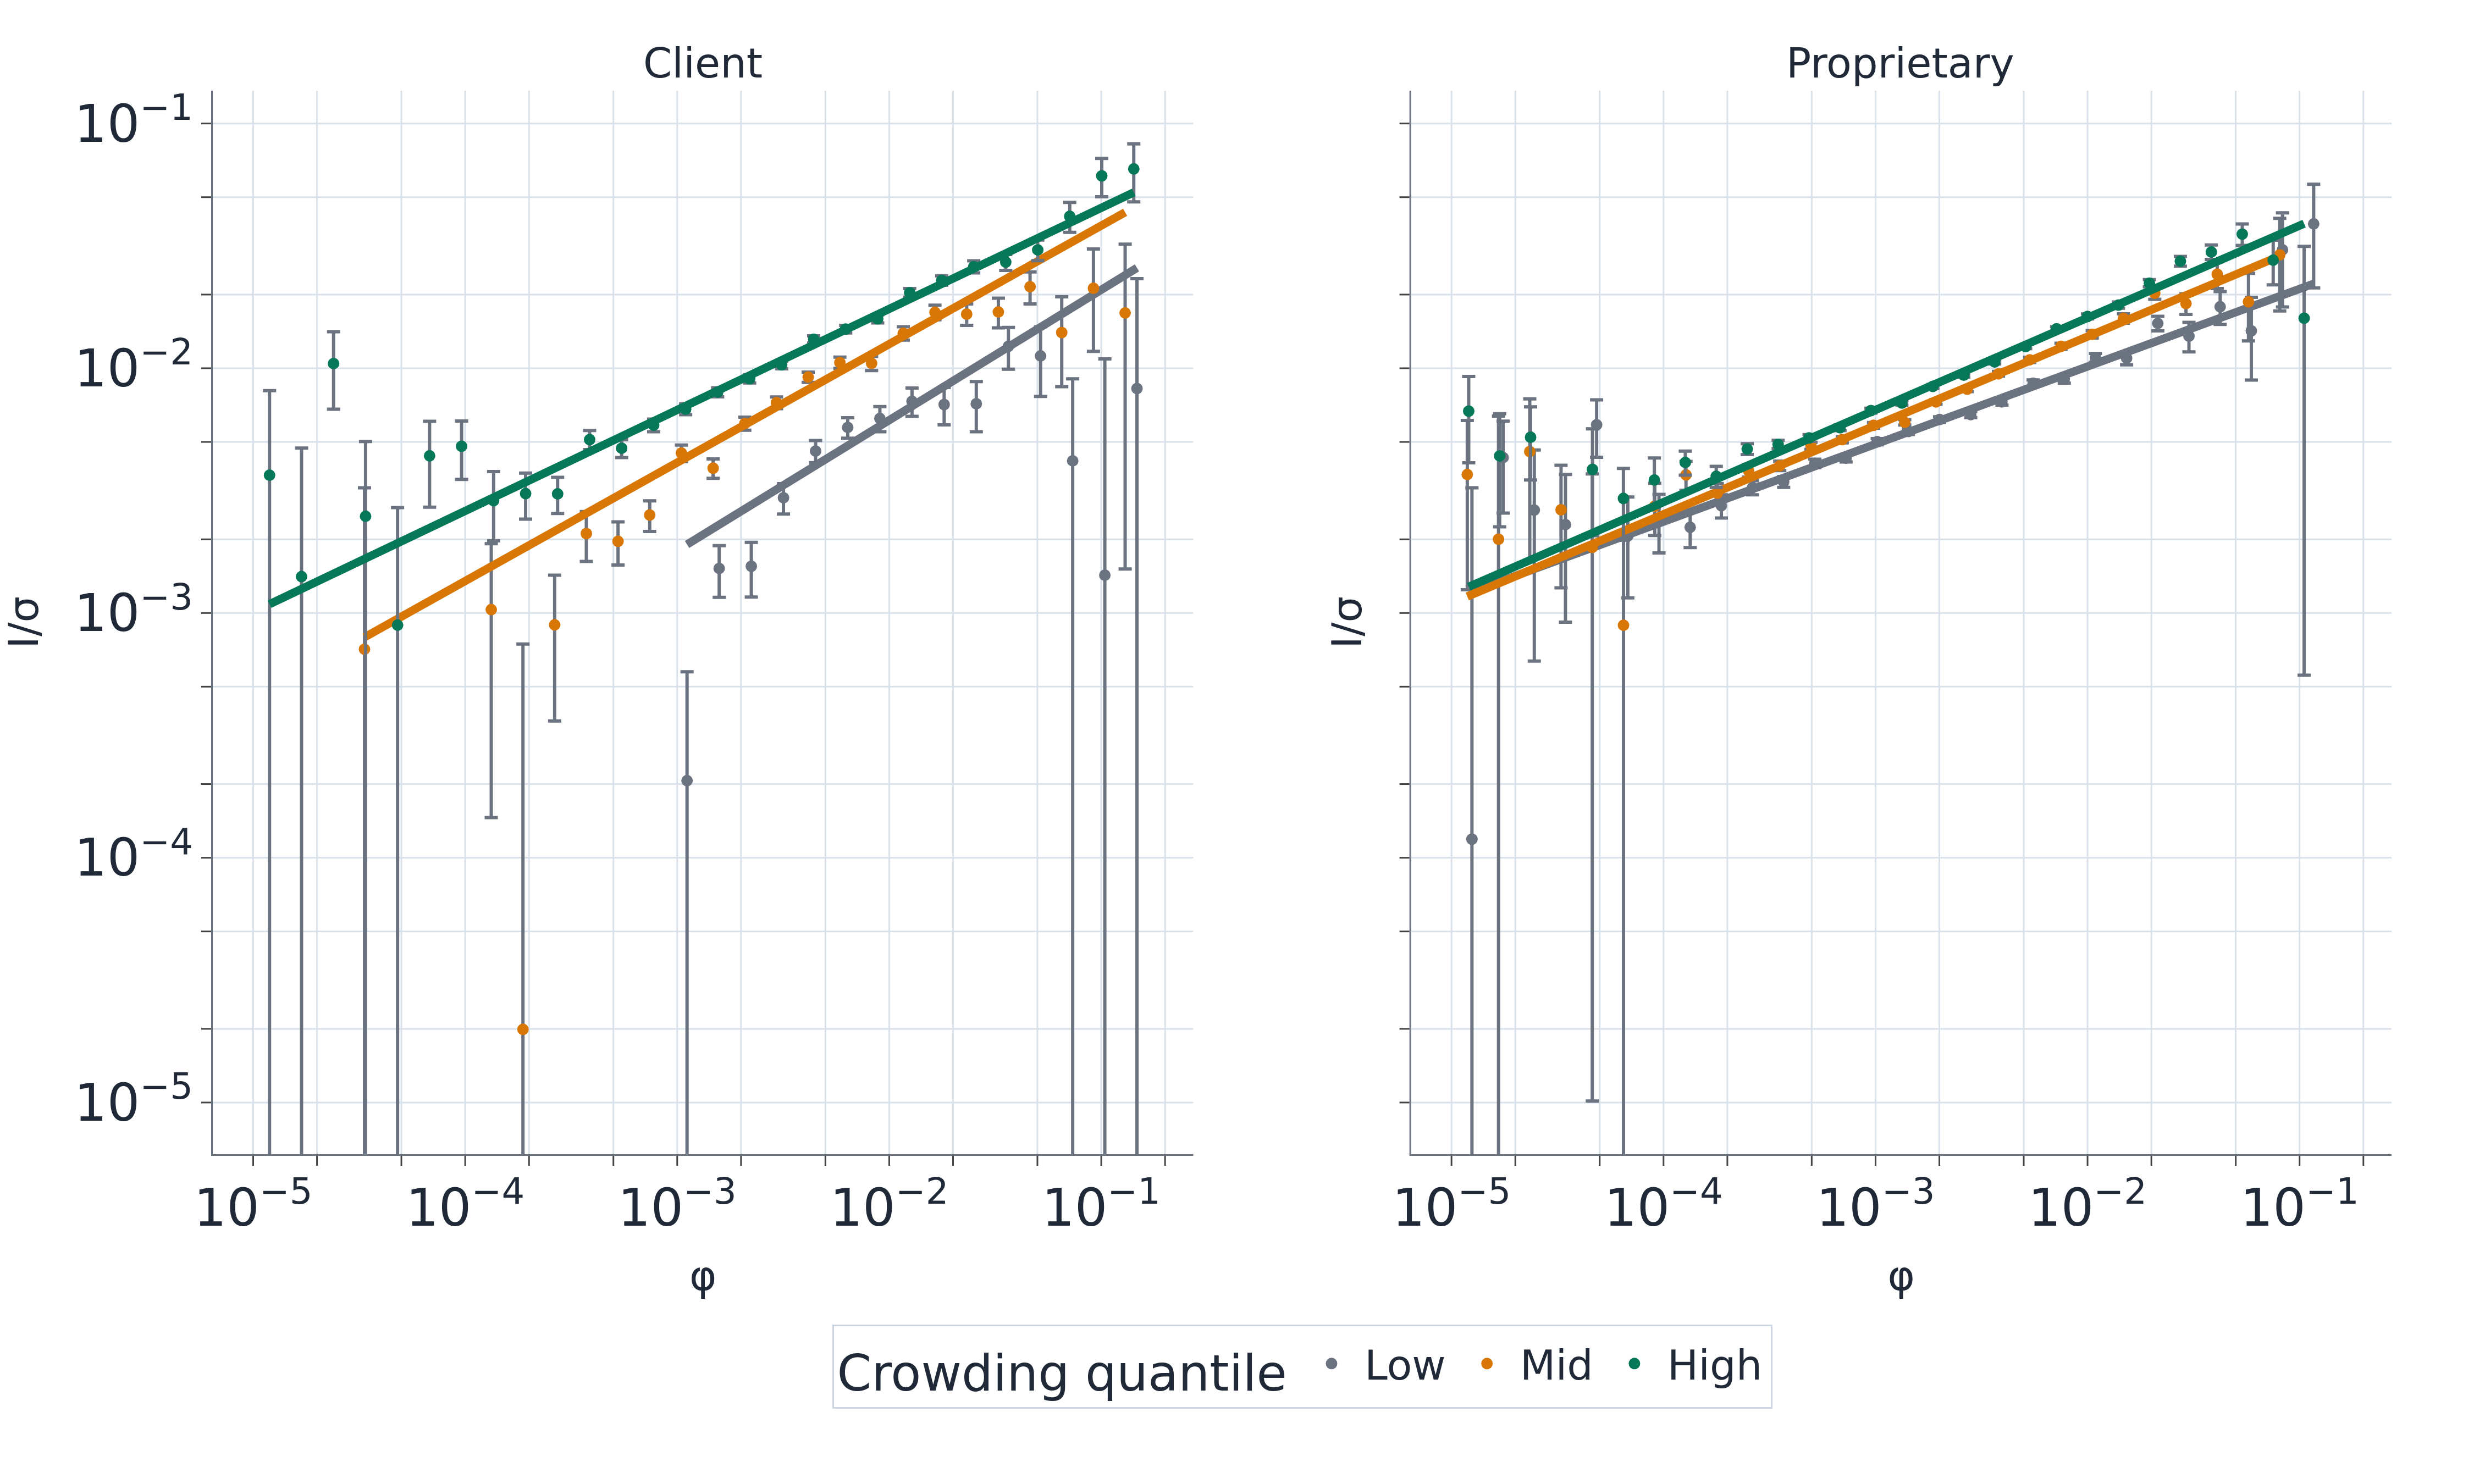
\includegraphics[width=0.75\textwidth]{images/crowding_impact/png/main_crowding_impact_curves.png}
  \caption{Impact curves by tercile of all-flow alignment \(a_i^{\mathrm{all}}\).}
  \label{fig:impact_curves_by_crowding}
\end{figure}

\begin{figure}
  \centering
  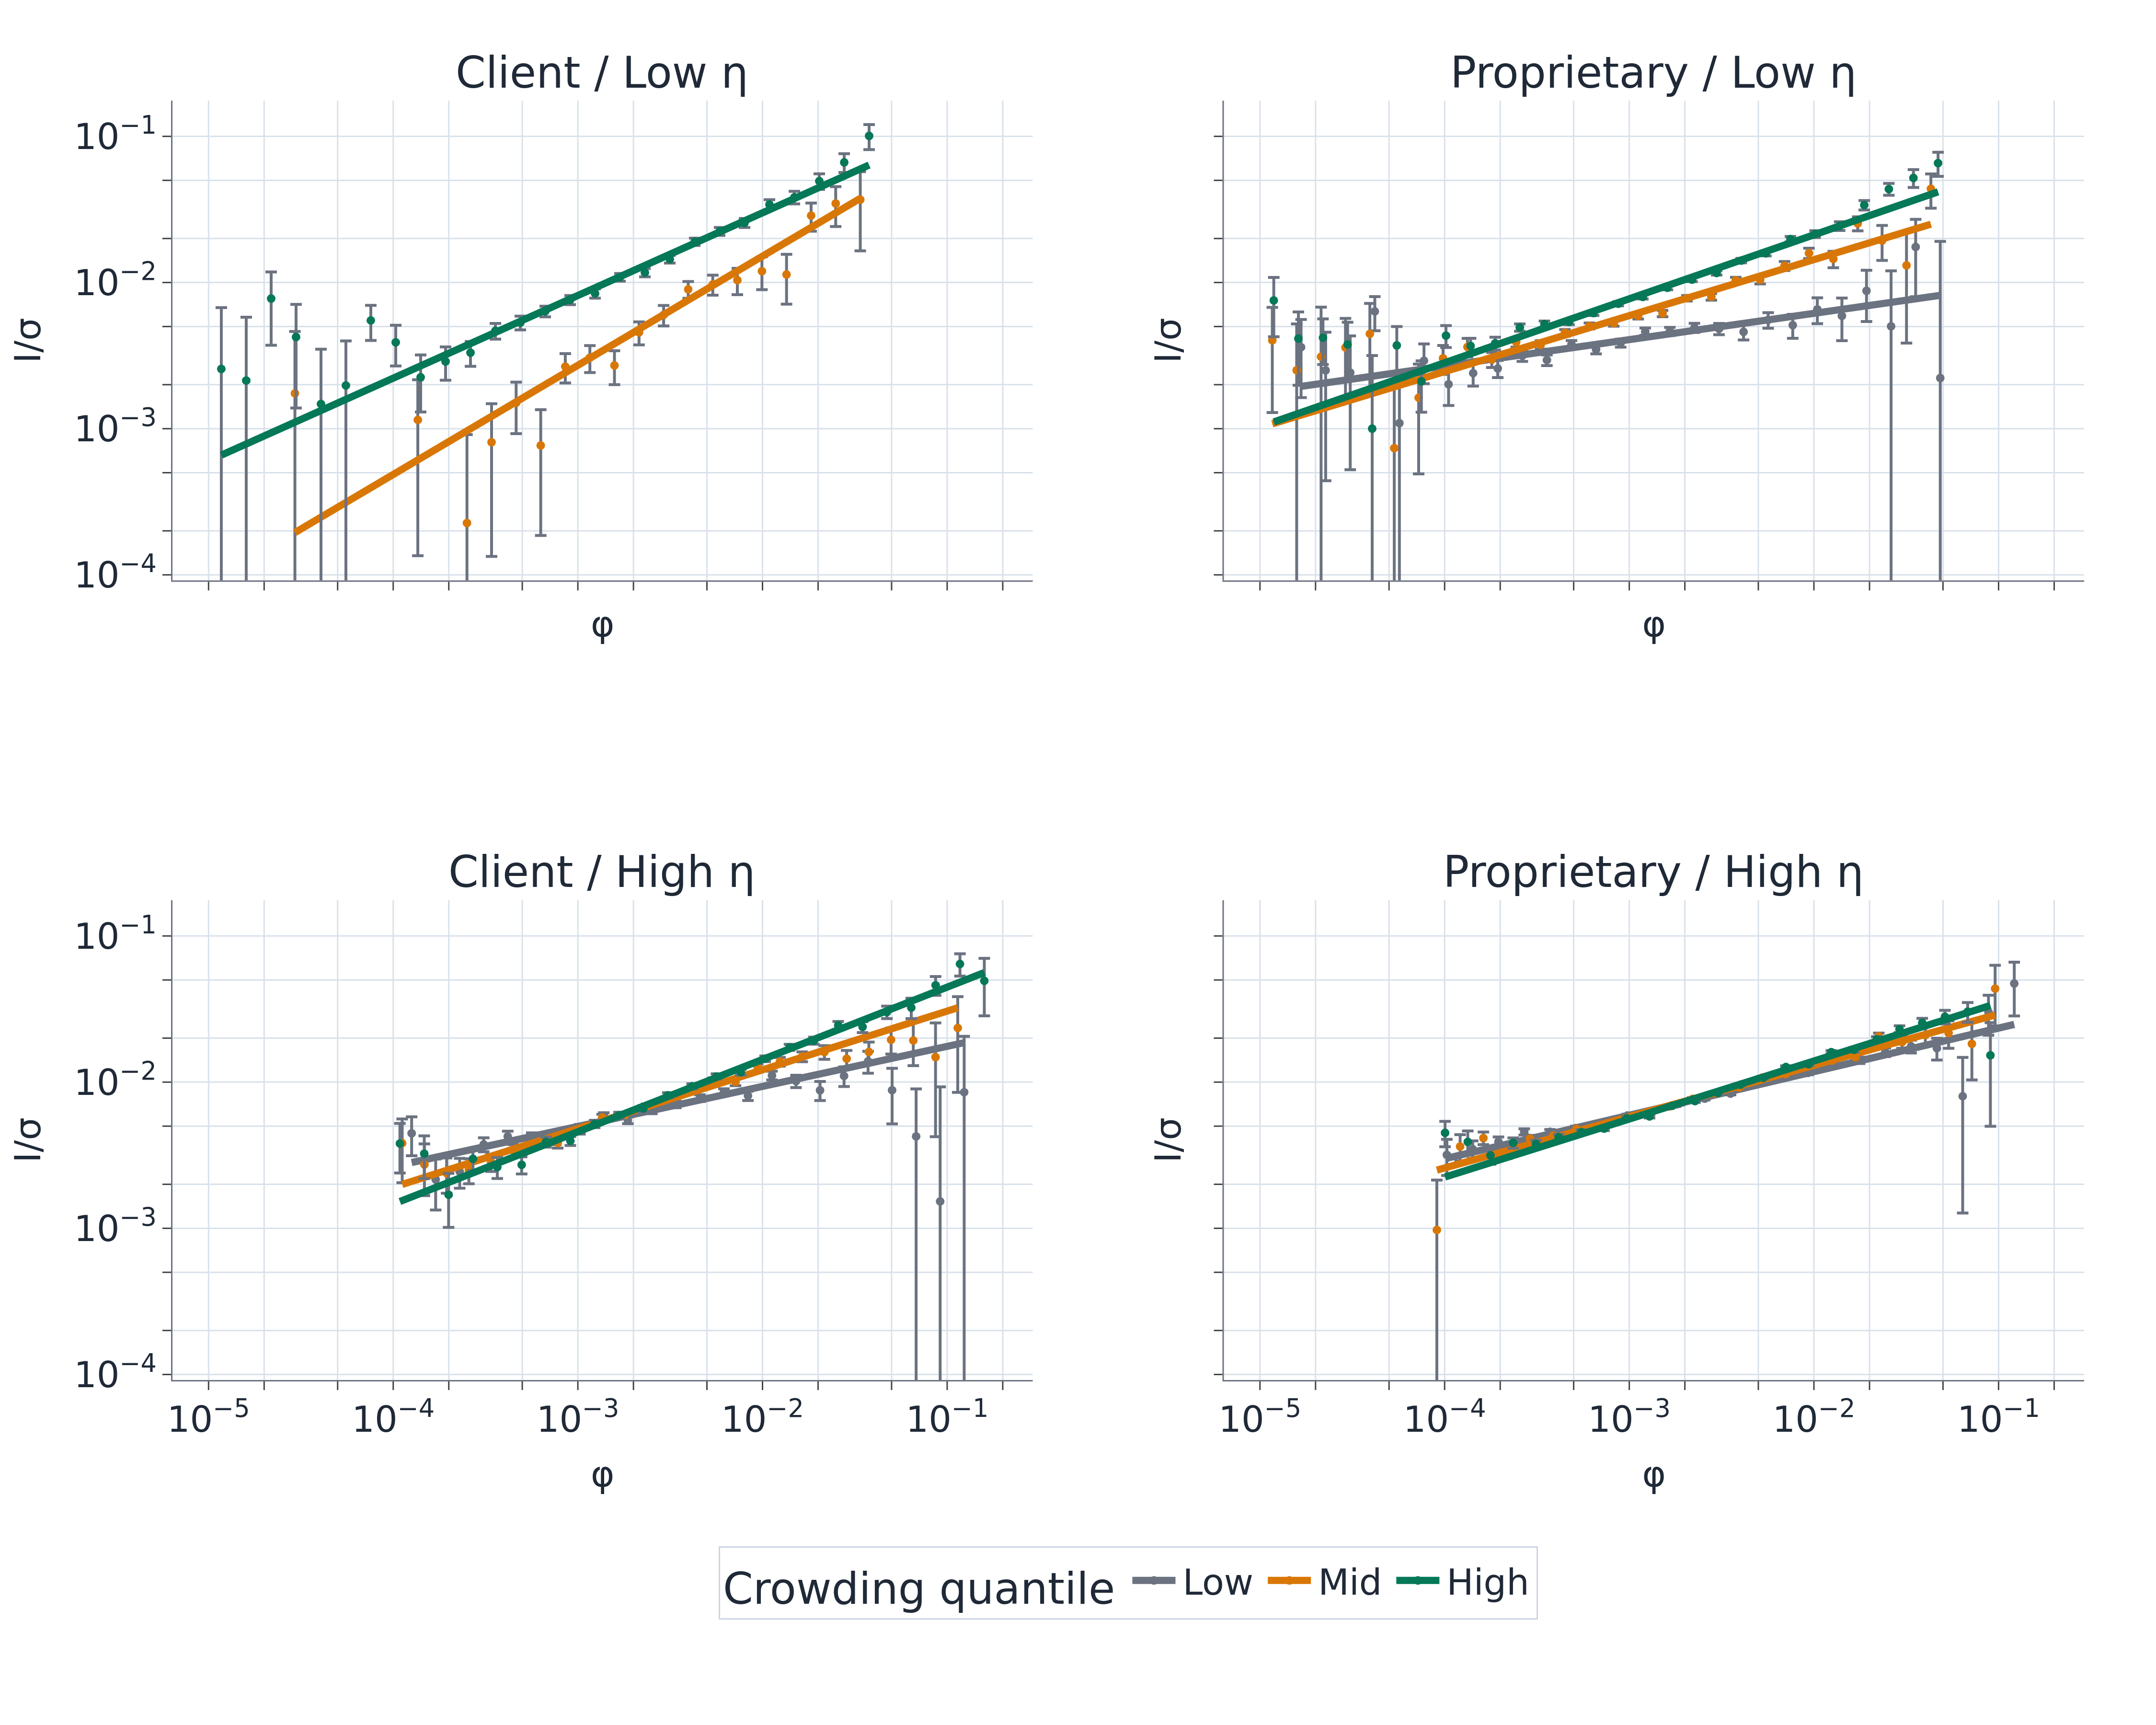
\includegraphics[width=0.9\textwidth]{images/crowding_impact/png/eta_robustness_crowding_impact_curves.png}
  \caption{Impact curves by tercile of all-flow alignment \(a_i^{\mathrm{all}}\), across two participation-rate bins.}
  \label{fig:impact_curves_by_crowding_and_eta}
\end{figure}

\begin{table}[t]
\centering
\scriptsize
\setlength{\tabcolsep}{4pt}
\begin{tabular}{@{}lcccc@{}}
\toprule
& \multicolumn{2}{c}{\(\phi = 10^{-3}\)} & \multicolumn{2}{c}{\(\phi = 10^{-2}\)} \\
Group & High \(-\) low & 95\% CI & High \(-\) low & 95\% CI \\
\midrule
Client & 0.00496 & [0.00448, 0.00579] & 0.01135 & [0.00968, 0.01285] \\
Proprietary & 0.00186 & [0.00155, 0.00213] & 0.00592 & [0.00502, 0.00684] \\
Prop.\ \(-\) client & -0.00310 & [-0.00377, -0.00272] & -0.00543 & [-0.00644, -0.00424] \\
\bottomrule
\end{tabular}
\caption{Difference between fitted impacts in the highest and lowest terciles of
all-flow alignment \(a_i^{\mathrm{all}}=\varepsilon_i m_i^{G_i,\mathrm{all}}\).
Positive values indicate that more crowded metaorders have higher fitted impact
at benchmark size \(\phi\). Confidence intervals are obtained from a day-cluster
bootstrap with 200 replicates.}
\label{tab:crowding_impact_terciles}
\end{table}

As a second daily-crowding check, we extend the regression analysis of normalized
impact versus metaorder relative size with imbalance magnitude and execution
state. Let \(v_i \equiv V_i^{\text{window}}/V_{d(i)} = \phi_i/\eta_i\) be the
metaorder duration in volume time. We form common pooled bins in
\((\eta_i, v_i, |m_i^{G_i,\mathrm{all}}|)\). In each retained positive-mean bin
\(b\), let \(\bar I_b\) be the mean signed impact, \(\eta_b\) and \(v_b\) the bin
means of \(\eta_i\) and \(v_i\), and
\(M_b^{\mathrm{all}}\) the bin mean of \(|m_i^{G_i,\mathrm{all}}|\). We estimate
\begin{equation}
  \log \bar I_b
  =
  \alpha
  + \beta_{\eta}\log \eta_b
  + \beta_v \log v_b
  + \beta_m M_b^{\mathrm{all}}
  + \beta_p \mathbf{1}\{G_b=\mathrm{prop}\}
  + \xi_b.
\end{equation}
As in the standard impact fits, the regression is estimated by WLS, with weights
based on the delta-method variance of \(\log \bar I_b\) computed from the
bin-level SEM. Table~\ref{tab:crowding_impact_pooled} shows the estimated
coefficients of the fit. We observe that \(M_b^{\mathrm{all}}\) enters
positively, but the proprietary dummy remains large and significant. The
estimate \(\hat\beta_p=0.173\) implies roughly \(19\%\) higher mean impact for
proprietary bin-level observations with the same participation rate,
execution-window volume share, and daily crowding magnitude. Daily imbalance is
therefore relevant for impact, but it does not absorb the proprietary impact
premium.

\begin{table}[t]
\centering
\scriptsize
\setlength{\tabcolsep}{4pt}
\begin{tabular}{@{}lccc@{}}
\toprule
Regressor & Estimate & Bootstrap 95\% CI \\
\midrule
\(\log \eta\) & 0.227 &  [0.216, 0.238] \\
\(\log v\) & 0.265 &  [0.258, 0.285] \\
\(M^{\mathrm{all}}\) & 0.084 &  [0.019, 0.142] \\
\(\mathbf{1}\{G=\mathrm{prop}\}\) & 0.173 &  [0.115, 0.221] \\
\bottomrule
\end{tabular}
\caption{Pooled bin-level regression of \(\log \bar I_b\) on execution-state
controls and crowding magnitude. Bins are formed using common intervals in
\((\eta, v, |m^{\mathrm{all}}|)\) across proprietary and client flow, with
\(v=\phi/\eta = V^{\text{window}}/V_d\). The variable \(M_b^{\mathrm{all}}\) is
the bin mean of \(|m_i^{G_i,\mathrm{all}}|\). The reported regression uses 111
retained bins out of 176 non-empty pooled bins. Bootstrap intervals are obtained
from a day-cluster bootstrap with 200 replicates.}
\label{tab:crowding_impact_pooled}
\end{table}

The daily-imbalance tests therefore point to a more local question. The impact
curves measure the price response during and after a metaorder; a relevant
crowding channel may therefore be the flow that is alive during the target
metaorder's execution, not only the same-day aggregate imbalance. For target
metaorder \(i\) and another metaorder \(j\) in the same \((\mathrm{ISIN},\mathrm{Date})\),
we define the active-overlap weight
\begin{equation}
  \omega_{ij}
  =
  \frac{
  \left[
  \min(t_i^{\text{end}},t_j^{\text{end}})
  -
  \max(t_i^{\text{start}},t_j^{\text{start}})
  \right]_+}
  {t_i^{\text{end}}-t_i^{\text{start}}}.
\end{equation}
With the convention that a zero-duration target has \(\omega_{ij}=1\) if
\(t_j^{\text{start}}\leq t_i^{\text{start}}\leq t_j^{\text{end}}\) and zero
otherwise. Let \(\mathcal{N}_i\) be the set of all other metaorders in the same
\((\mathrm{ISIN},\mathrm{Date})\) as target \(i\). We compute:
\begin{itemize}
  \item the active count
  \(n_i^{\mathrm{act}}=\sum_{j\in\mathcal{N}_i}\omega_{ij}\);
  \item the gross active volume normalized by target size
  \(h_i^{\mathrm{act}}=\sum_{j\in\mathcal{N}_i}\omega_{ij}Q_j/Q_i\);
  \item the same-sign and opposite-sign active volumes
  \(S_i^{\mathrm{act}}=\sum_{j\in\mathcal{N}_i:\varepsilon_j=\varepsilon_i}\omega_{ij}Q_j\)
  and
  \(O_i^{\mathrm{act}}=\sum_{j\in\mathcal{N}_i:\varepsilon_j=-\varepsilon_i}\omega_{ij}Q_j\);
  \item the target-signed active imbalance
  \(B_i^{\mathrm{act}}=(S_i^{\mathrm{act}}-O_i^{\mathrm{act}})/
  (S_i^{\mathrm{act}}+O_i^{\mathrm{act}})\).
\end{itemize}

Table~\ref{tab:active_overlap_summary} summarizes the resulting features.
Proprietary targets are not more overlapped in count: the mean time-weighted
active count is \(5.36\) for proprietary metaorders and \(5.57\) for client
metaorders. Gross active volume normalized by target size is also not higher for
proprietary targets. The statistic that distinguishes the groups is directional:
target-signed active imbalance is positive for proprietary metaorders and close
to zero for clients. Thus the active-overlap evidence refines the daily-crowding
evidence. Proprietary metaorders are not executed in a mechanically denser local
daily environment, but the overlapping flow they face is more often aligned with
their own direction.

\begin{table}[t]
\centering
\scriptsize
\setlength{\tabcolsep}{4pt}
\begin{tabular}{@{}lrrrr@{}}
\toprule
Active-overlap feature & Client mean & Client median & Prop. mean & Prop. median \\
\midrule
Time-weighted active count & 5.57 & 5.40 & 5.36 & 5.15 \\
Gross active volume / target \(Q\) & 36.66 & 10.90 & 25.55 & 11.14 \\
Target-signed active imbalance & 0.000 & 0.001 & 0.026 & 0.038 \\
Same-sign active volume & 177{,}728 & 33{,}959 & 172{,}275 & 32{,}098 \\
Opposite-sign active volume & 183{,}110 & 33{,}344 & 153{,}453 & 28{,}795 \\
\bottomrule
\end{tabular}
\caption{Active-overlap features computed over true execution intervals within
the same ISIN and date. The target itself is excluded. The active imbalance is
signed by the target direction, so positive values indicate that the overlapping
flow is aligned with the target metaorder.}
\label{tab:active_overlap_summary}
\end{table}

We quantify this channel by estimating three controlled versions of the
log-binned WLS impact curves by adding additional regressors each time. The
baseline WLS specification includes the proprietary dummy and \(\log(Q/V)\); we
then add the logs of bin-mean participation and volume duration. Finally, we add
positive active-overlap components: the log of bin-mean active count, same-sign
active overlap normalized by target size, and opposite-sign active overlap
normalized by target size. Table~\ref{tab:active_overlap_wls_regression} reports
the proprietary log-coefficient.

\begin{table}[t]
\centering
\scriptsize
\setlength{\tabcolsep}{3pt}
\begin{tabular}{@{}lp{0.34\textwidth}rrrrr@{}}
\toprule
Model & Controls & \(\hat\beta_{\mathrm{prop}}\) & \(\exp(\hat\beta)-1\) & 95\% CI & Bins & \(N\) \\
\midrule
W0 & \(\log(Q/V)\) & 0.179 & 19.6\% & [0.114, 0.245] & 51 & 833{,}795 \\
W1 & W0 plus \(\log(\bar\eta)\) and \(\log(\bar v)\) & 0.182 & 20.0\% & [0.072, 0.292] & 51 & 833{,}795 \\
W2 & W1 plus positive active-overlap controls & 0.140 & 15.0\% & [-0.065, 0.344] & 51 & 833{,}795 \\
\bottomrule
\end{tabular}
\caption{Power-law-style binned log-WLS regressions. The dependent variable is
the log mean impact in group-by-\(Q/V\) bins. W2 adds the log of positive
bin-mean active-overlap controls to the binned WLS specification.}
\label{tab:active_overlap_wls_regression}
\end{table}

This exercise answers the question closest to the original impact-curve
evidence. Participation rate and duration alone do not reduce the proprietary
log-premium: W0 and W1 give similar coefficients, about \(0.18\), or a \(20\%\)
multiplicative premium. Once active-overlap summaries are added on the same 51
\(Q/V\) curve bins, the coefficient falls to \(0.14\) and the confidence interval
includes zero. This shows that, in the same log-binned WLS language used in
Section~\ref{subsec:impact_models}, active directional overlap is the control
that most weakens the proprietary premium.

Putting these pieces together, crowding is relevant for impact, but the channel
is not simply the number of simultaneous metaorders. Daily crowding is stronger
for clients, and active overlap in counts and gross volume is not higher for
proprietary targets. What distinguishes proprietary executions is the sign of
the active environment. Active directional overlap explains part of the
proprietary coefficient at the metaorder level and materially weakens it in the
power-law-style binned WLS. We therefore interpret the higher proprietary impact
as partly associated with execution in more directionally aligned local
environments, while recognizing that the residual magnitude depends on the
aggregation level and controls used.

\section{Member--client interactions}
\label{sec:member_prop_client_alignment}

The preceding section focuses on whether crowding helps explain the aggregate proprietary impact
premium. We now separate a related but distinct question: whether a member's proprietary metaorders
are directionally aligned with the client flow executed through the same member. This analysis is a
diagnostic of prop--client interaction, not a direct test of the aggregate impact premium. Positive
alignment is consistent with co-movement that may amplify client flow and can raise patterns deserving 
further analytical scrutiny, as they may be consistent with a variety of mechanisms, including common 
information, execution synchronization, inventory management practices and, in some cases, behaviours 
that may warrant closer supervisory attention; negative alignment is consistent with client facilitation, 
inventory absorption, or risk transfer. In either case, the measures are descriptive and cannot establish intent.

\subsection{Daily member-level prop--client alignment}
\label{subsec:member_level_crowding}
We first measure prop--client alignment at the member-day level. The object is the correlation
between a member's proprietary trading direction and the order-flow imbalance generated by the
clients whose metaorders were executed through that same member.

For a given member $m$ and date $d$, let $\mathcal{C}_{m,d}$ denote the set of client metaorders executed 
by member $m$ on day $d$, aggregated across all ISINs. We define the member-level client imbalance as
\begin{equation}
\text{imb}_{m,d}
  = \frac{\sum_{j \in \mathcal{C}_{m,d}} Q_j \epsilon_j}
         {\sum_{j \in \mathcal{C}_{m,d}} Q_j},
\end{equation}
where $Q_j$ and $\epsilon_j$ denote, respectively, the size and direction of client metaorder $j$.
The statistic $\text{imb}_{m,d}$ is considered valid only when both the member and its associated 
client cohort initiate a sufficient number of metaorders during day $d$. Using members with at least 30 proprietary and 
30 client metaorders over the sample, there are $10$ such members (out of 45), and the mean per-member correlation 
between proprietary direction and client imbalance is shown in Figure \ref{fig:hist_imbcorr}. As we can see,
most members have correlations close to zero, but a few exhibit stronger positive or negative correlations with
peak values near $+0.4$ suggesting 
that the relationship between proprietary trading and client flow is quite heterogeneous across members and not trivial.

% Aggregating across all member-level observations, the global correlation between proprietary direction and the 
% member-level client imbalance is $0.011$ with a bootstrap $95\%$ CI $[0.001, 0.022]$ and a permutation p-value $p=0.014$.

To assess whether prop--client alignment is episodic, we also compute the same correlation over
non-overlapping 3-day windows. Large positive values indicate periods in which proprietary flow
moves with same-member client imbalance; large negative values indicate periods in which it moves
against that imbalance. Figure~\ref{fig:heatmap_imbcorr} reports the resulting heatmap. 
The white vertical gaps are not zero-correlation periods: they correspond to windows in which no displayed member has
enough proprietary and same-member client activity to pass the minimum-count filter, so the member-window correlation is undefined and the entry is omitted.
As illustrated, most member-window blocks hover near zero, but a handful of windows show stronger 
alignment or opposition (often in small-sample windows), suggesting that prop--client co-movement is 
episodic and member-dependent rather than uniformly persistent.

\begin{figure}
    \centering
    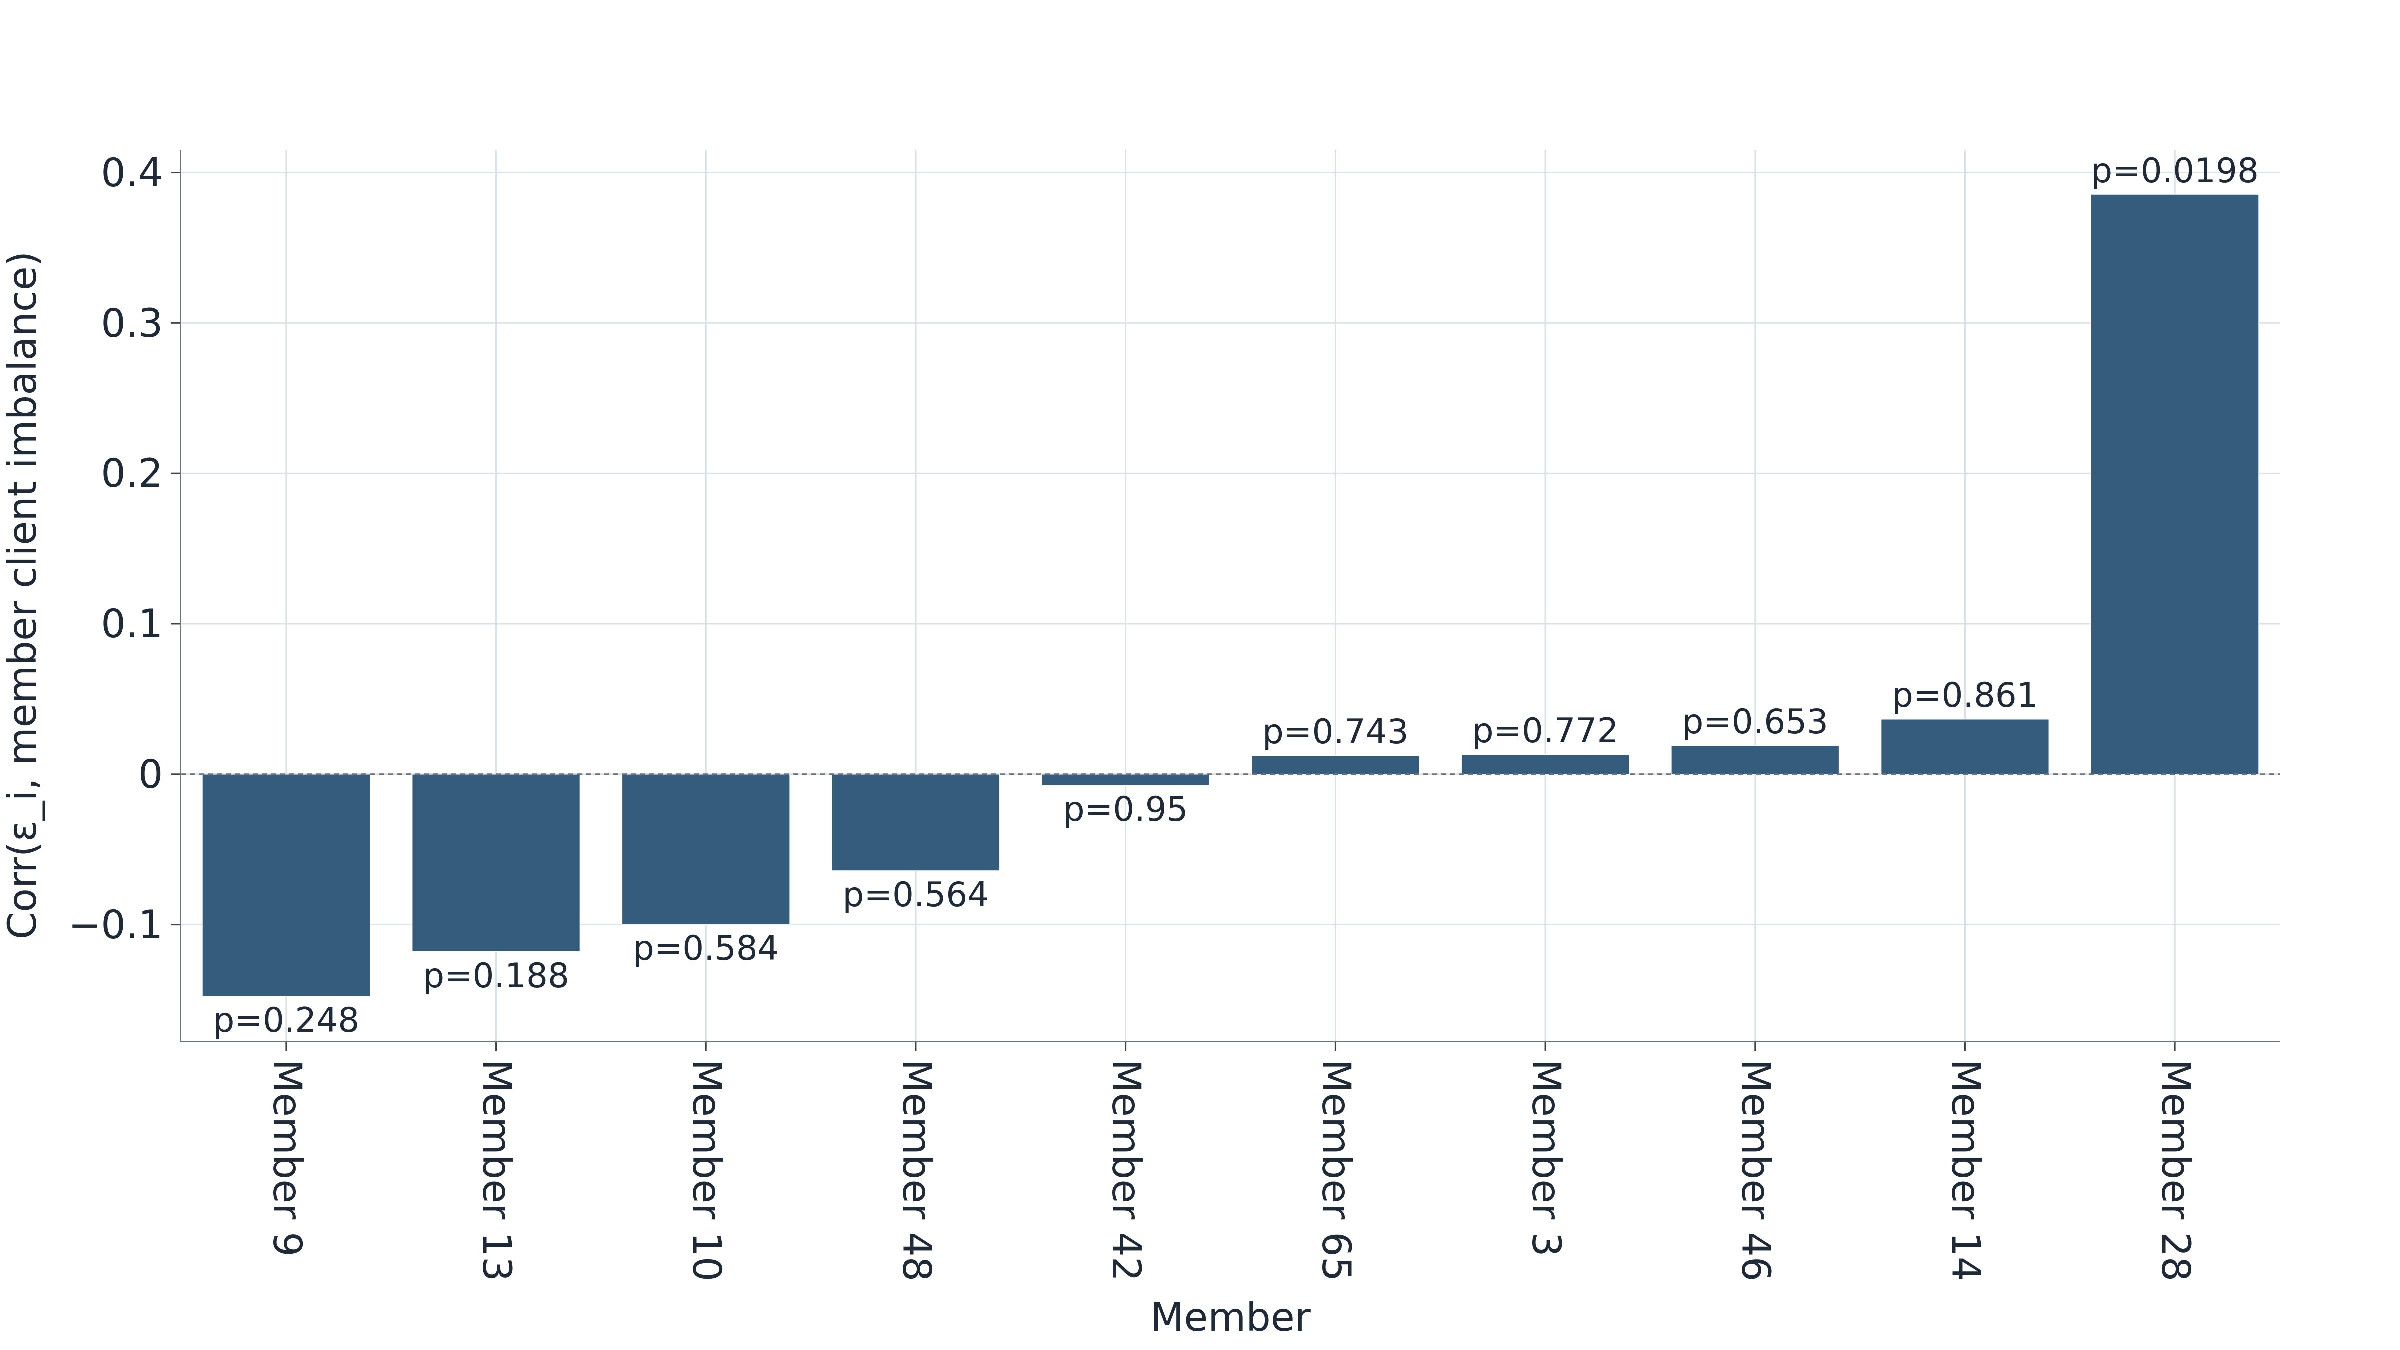
\includegraphics[width=0.75\linewidth]{images/prop_vs_nonprop/png/member_prop_client_crowding_hist}
    \caption{Per-member correlations between proprietary trading direction and member-level client imbalance (members 
    with at least 30 proprietary and 30 client metaorders; horizontal line marks zero).}
    \label{fig:hist_imbcorr}
\end{figure}

\begin{figure}
    \centering
    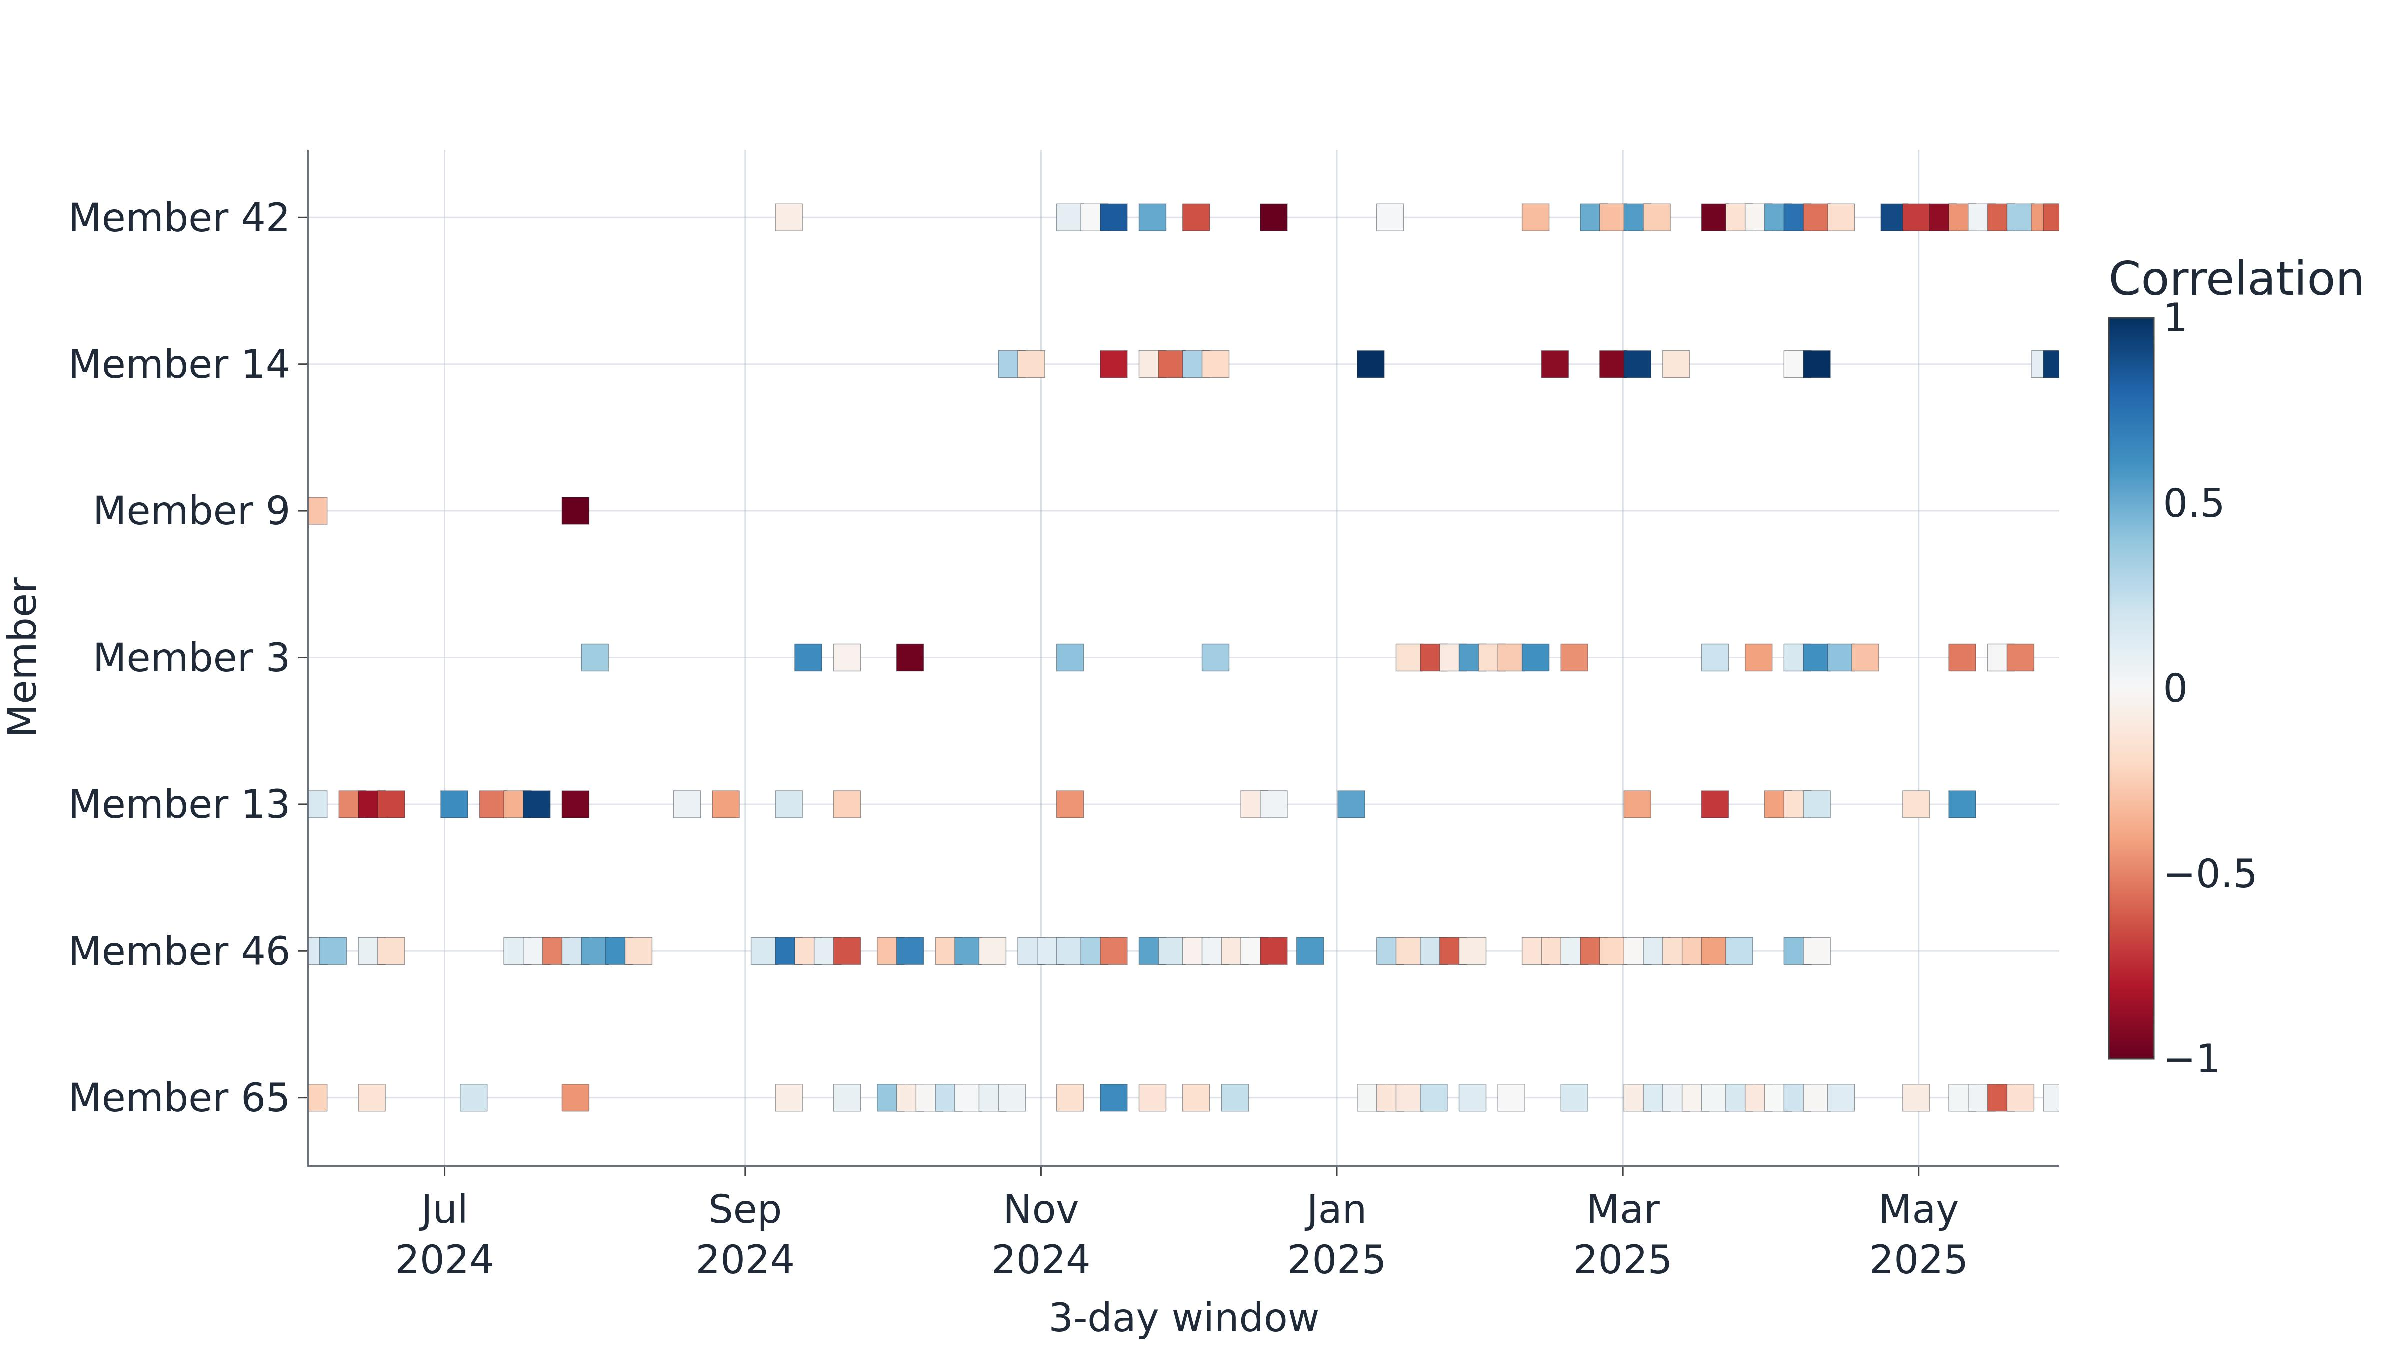
\includegraphics[width=1\linewidth]{images/prop_vs_nonprop/png/member_prop_client_crowding_heatmap_3d}
    \caption{Sparse heatmap of the correlation between proprietary metaorder directions and the same-member client
order-flow imbalance, computed over non-overlapping 3-day windows. Only member-window entries passing the minimum-count
filter are shown: both the proprietary desk and its client cohort must execute at least 5 metaorders in that window.
Members with no displayed entries are omitted. Colors indicate the sign and magnitude of
$\mathrm{corr}(\epsilon_i, \mathrm{imb}_{m,d})$, with blue (red) denoting positive (negative) association.
The figure highlights several members exhibiting episodic periods of stronger alignment or opposition.}
    \label{fig:heatmap_imbcorr}
\end{figure}


\subsection{Active same-member prop--client alignment during execution}
\label{subsec:member_active_overlap_crowding}

We next make the member-level alignment test local in execution time. The active-overlap results
in Section~\ref{subsec:crowding_impact} suggest that the flow alive during the execution interval
is the relevant local environment. We therefore return to the member-level question of
Section~\ref{subsec:member_level_crowding}: are there members whose proprietary metaorders are
systematically aligned, either positively or negatively, with the flow of their own clients? The
difference with the member-day statistic is that the client environment is now restricted to active
overlapping client metaorders.

For a proprietary metaorder $i$ executed by member $m$, let
$\mathcal{C}^{\mathrm{act}}_{i,m}$ be the set of client metaorders executed
through the same member, on the same ISIN and date, that overlap in calendar
time with $i$. Using the active-overlap weights $\omega_{ij}$ defined above, the
active client imbalance faced by $i$ is
\begin{equation}
  \mathrm{imb}^{\mathrm{act}}_{i,m}
  =
  \frac{\sum_{j\in\mathcal{C}^{\mathrm{act}}_{i,m}}\omega_{ij}Q_j\epsilon_j}
       {\sum_{j\in\mathcal{C}^{\mathrm{act}}_{i,m}}\omega_{ij}Q_j},
  \label{eq:member_active_imbalance}
\end{equation}
and is left undefined when the denominator is zero. This is the active,
same-ISIN analogue of $\mathrm{imb}_{m,d}$ in
Section~\ref{subsec:member_level_crowding}. The member-specific statistic is
\begin{equation}
  r_m^{\mathrm{act}}
  =
  \mathrm{Corr}\!\left(
    \epsilon_i^{\mathrm{prop}},
    \mathrm{imb}^{\mathrm{act}}_{i,m}
    \,\middle|\, \mathrm{Member}(i)=m
  \right).
  \label{eq:member_active_corr}
\end{equation}
Positive values mean that the proprietary metaorders of member $m$ tend to have
the same sign as the active imbalance generated by its own clients; negative
values indicate systematic opposition. We also compute the signed alignment
$a_i=\epsilon_i^{\mathrm{prop}}\mathrm{imb}^{\mathrm{act}}_{i,m}$ as a
descriptive quantity. The correlation in \eqref{eq:member_active_corr} is more
stringent than the average of $a_i$, because it removes unconditional buy/sell
biases of the proprietary desk and of the client environment.

The local restriction is severe. Out of $588{,}334$ proprietary metaorders,
only $2{,}320$ have a same-member, same-ISIN client metaorder actively
overlapping in time. Table~\ref{tab:member_active_overlap_global} reports pooled
benchmark correlations. The baseline active-overlap correlation is positive but
small, $r^{\mathrm{act}}=0.036$, with a Date-cluster bootstrap confidence
interval including zero. Splitting the client environment by timing gives the
same qualitative message: the correlation is $0.051$ when the client metaorder
is already active at the proprietary start and $0.037$ when the client metaorder
starts during the proprietary interval. Thus the pooled evidence does not point
to a uniform member-level tendency to align with own-client flow.

\begin{table}[t]
\centering
\scriptsize
\setlength{\tabcolsep}{4pt}
\begin{tabular}{@{}llrrrr@{}}
\toprule
Environment & Timing bucket & Correlation & 95\% CI & Valid targets & Members \\
\midrule
same ISIN & all active & 0.036 & $[-0.032,\,0.104]$ & 2,320 & 12 \\
same ISIN & active at prop start & 0.051 & $[-0.034,\,0.137]$ & 1,446 & 11 \\
same ISIN & starts during prop & 0.037 & $[-0.038,\,0.105]$ & 1,225 & 12 \\
all ISINs & all active & 0.011 & $[-0.055,\,0.077]$ & 20,636 & 15 \\
\bottomrule
\end{tabular}
\caption{Pooled active member-level prop--client correlations. The main
environment is same-member, same-ISIN active client flow. The all-ISIN row is a
robustness check that pools active same-member client metaorders across
instruments. Confidence intervals are Date-cluster bootstrap percentile
intervals.}
\label{tab:member_active_overlap_global}
\end{table}

The pooled statistic can mask heterogeneity across members, which is the main
object of this exercise. We therefore compute \eqref{eq:member_active_corr}
separately by member and report members with at least 30 valid proprietary
targets in the relevant environment. In the baseline same-ISIN, all-active
specification, five members pass this threshold. Table~\ref{tab:member_active_overlap_members}
shows that most of them have correlations close to zero, but Member 42
stands out with $r_m^{\mathrm{act}}=0.431$ and a confidence interval
$[0.249,0.614]$. Member 13 is also positive, although its baseline interval
barely includes zero. We do not observe a comparable strongly negative
same-ISIN member in this specification.

\begin{table}[t]
\centering
\scriptsize
\setlength{\tabcolsep}{4pt}
\begin{tabular}{@{}lrrrr@{}}
\toprule
Member & $r_m^{\mathrm{act}}$ & 95\% CI & Valid targets & Dates \\
\midrule
Member 9  & -0.019 & $[-0.339,\,0.265]$ & 50  & 35 \\
Member 13 &  0.177 & $[-0.009,\,0.388]$ & 195 & 104 \\
Member 14 & -0.006 & $[-0.117,\,0.084]$ & 946 & 68 \\
Member 42 &  0.431 & $[0.249,\,0.614]$  & 89  & 61 \\
Member 65 &  0.033 & $[-0.075,\,0.156]$ & 981 & 162 \\
\bottomrule
\end{tabular}
\caption{Per-member active prop--client correlations in the main same-ISIN,
all-active environment. Members are shown when they have at least 30 valid
proprietary targets with an active same-member client environment.}
\label{tab:member_active_overlap_members}
\end{table}

The timing decomposition clarifies where the strongest member-specific signals
come from. For Member 42, the correlation remains positive when the client
metaorder is already active at the proprietary start:
$r_m^{\mathrm{act}}=0.382$ with 95\% CI $[0.059,0.685]$ over 34 valid targets.
The same member also has a large correlation in the ``starts during prop''
bucket ($0.501$, 95\% CI $[0.273,0.719]$, 62 targets). Member 13 is positive
in the latter bucket as well ($0.269$, 95\% CI $[0.079,0.451]$, 99 targets).
The first of these results is the most directly connected to alignment with
already active client flow; the latter two indicate local co-movement, but do
not establish that proprietary trading follows client flow, since the client
metaorders start after the proprietary interval has begun.

To make the strongest member-level correlations visually interpretable, we also
aggregate the target-level quantities into non-overlapping 5-trading-day
windows for the two members with the largest positive global correlations. For
member $m$ and window $w$, we plot the proprietary target-direction imbalance
and the average active client imbalance,
\[
P_{m,w}=n_{m,w}^{-1}\sum_i \epsilon_i^{\mathrm{prop}},
\qquad
C_{m,w}=n_{m,w}^{-1}\sum_i \mathrm{imb}^{\mathrm{act}}_{i,m},
\]
where the sums run over valid proprietary targets in that member-window. Unlike
the discarded member-window heatmap, this diagnostic imposes no minimum count
filter at the window level; sparse windows are simply reflected in the number of
targets reported in the figure metadata. We therefore use this panel only as a
descriptive co-movement diagnostic; the inferential object remains the
target-level correlation with bootstrap confidence intervals.

\begin{figure}[t]
  \centering
  \begin{subfigure}{0.85\textwidth}
    \centering
    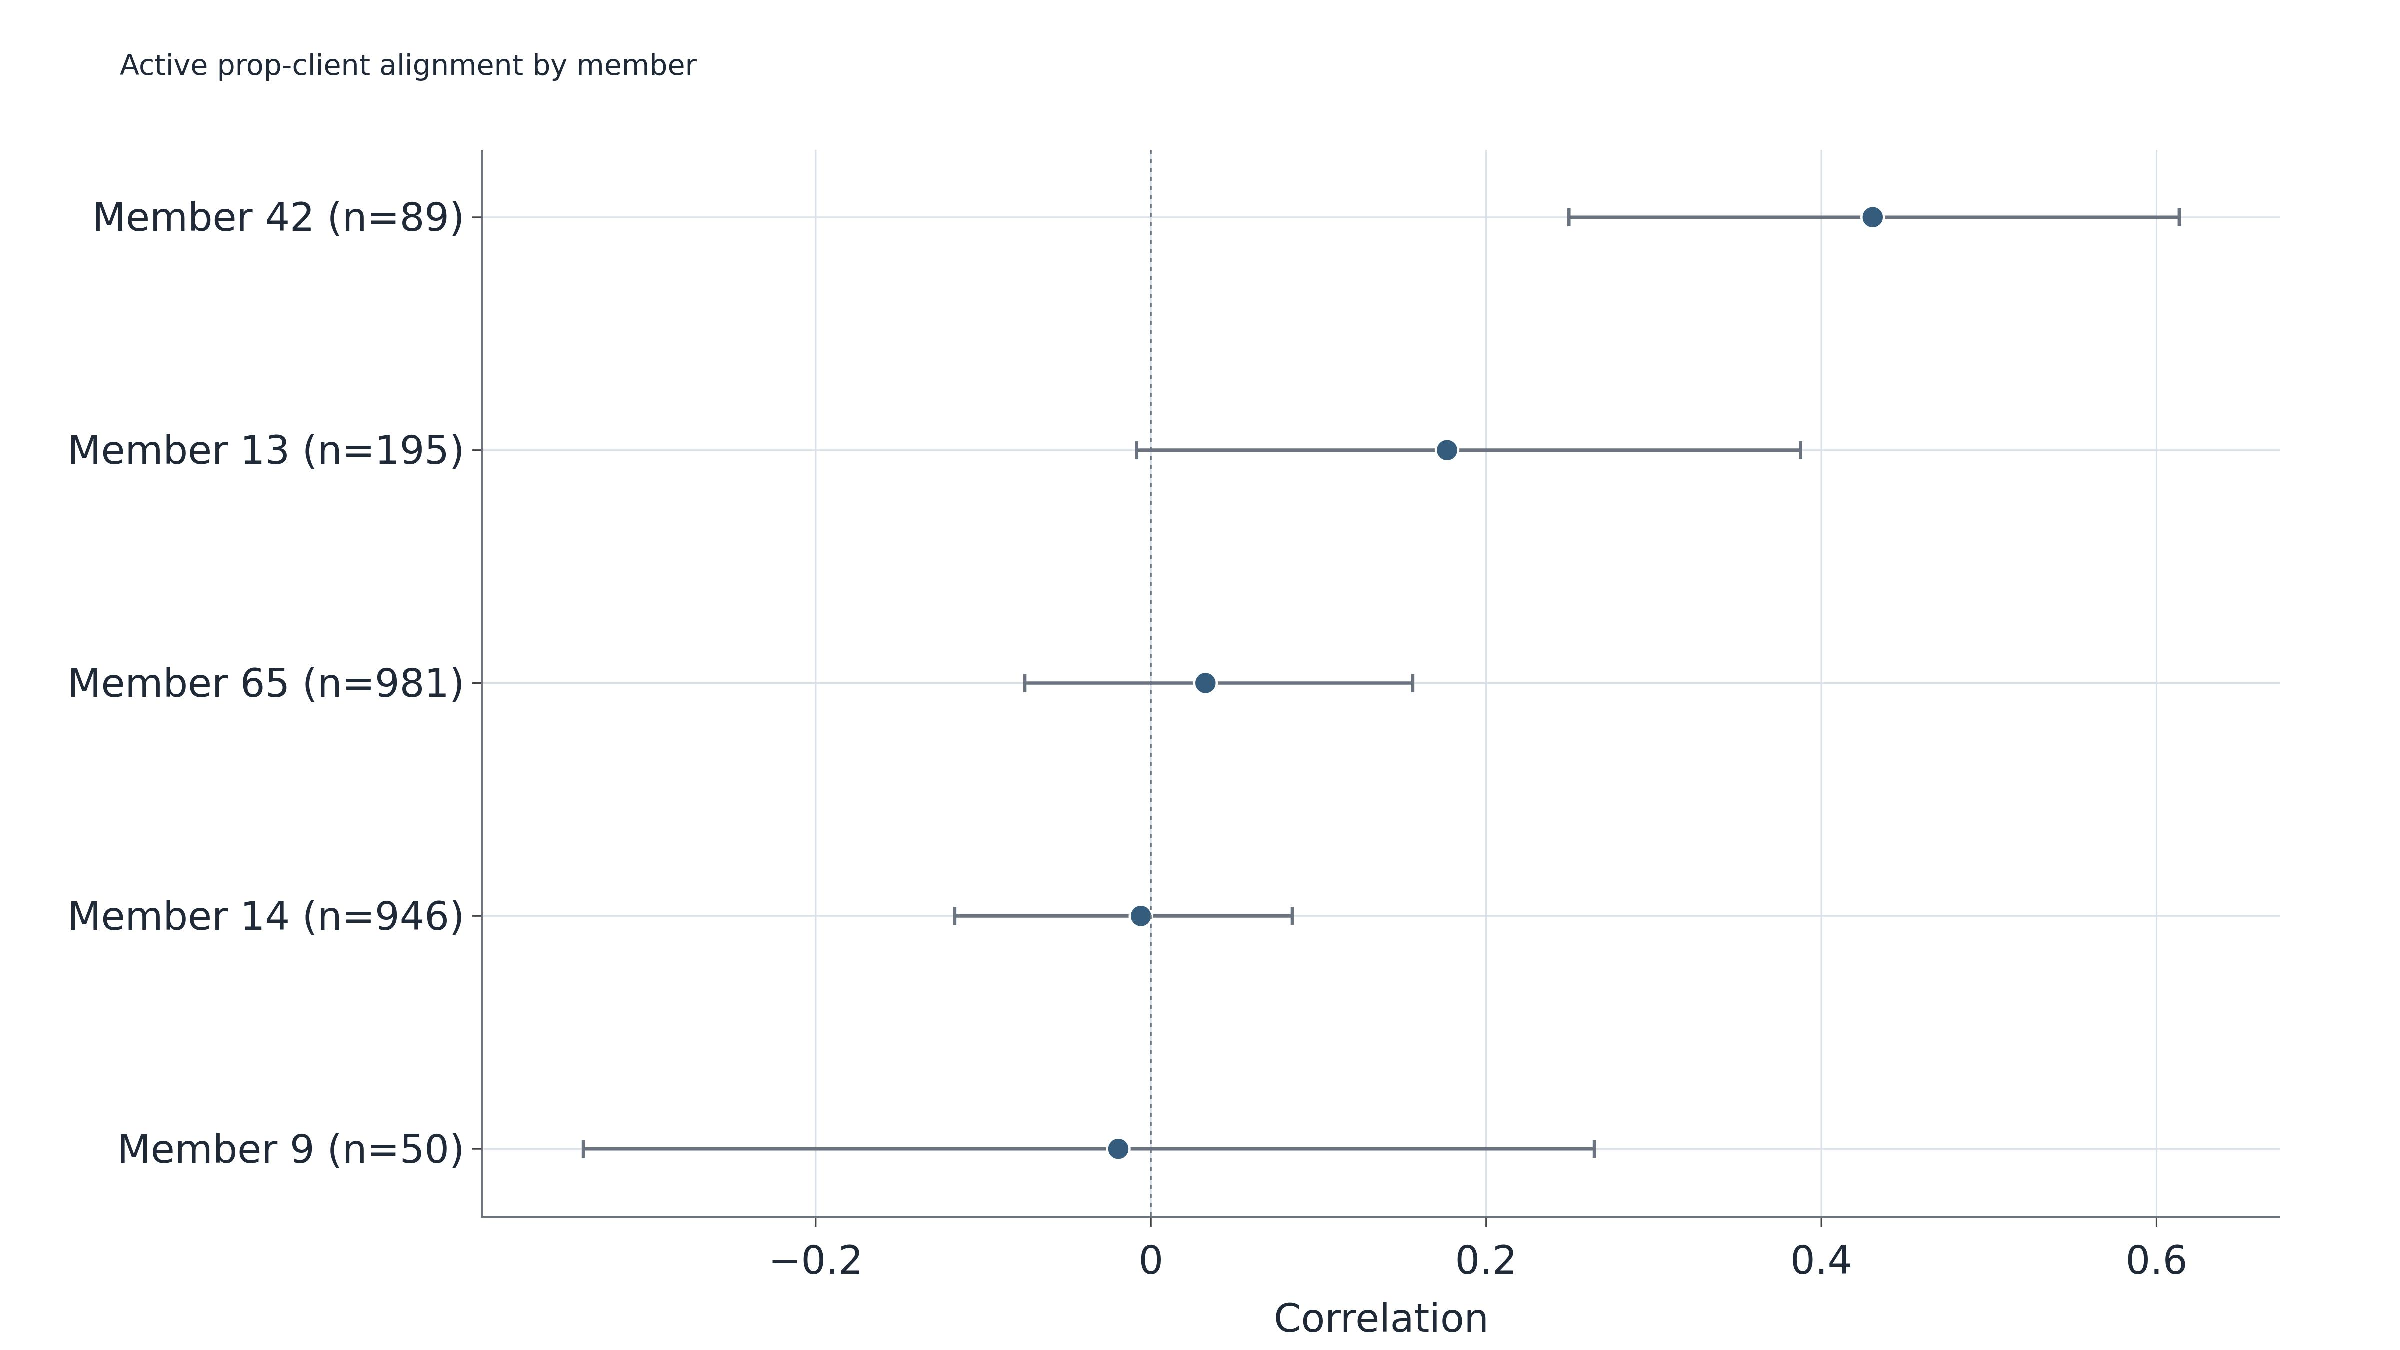
\includegraphics[width=\textwidth]{images/member_active_overlap_crowding/png/per_member_correlations_same_isin_all_active}
    \caption{Per-member correlations, same-ISIN all-active environment. Points show $r_m^{\mathrm{act}}$ and horizontal bars show 95\% bootstrap confidence intervals.}
  \end{subfigure}
  \vspace{0.5em}
  \begin{subfigure}{0.95\textwidth}
    \centering
    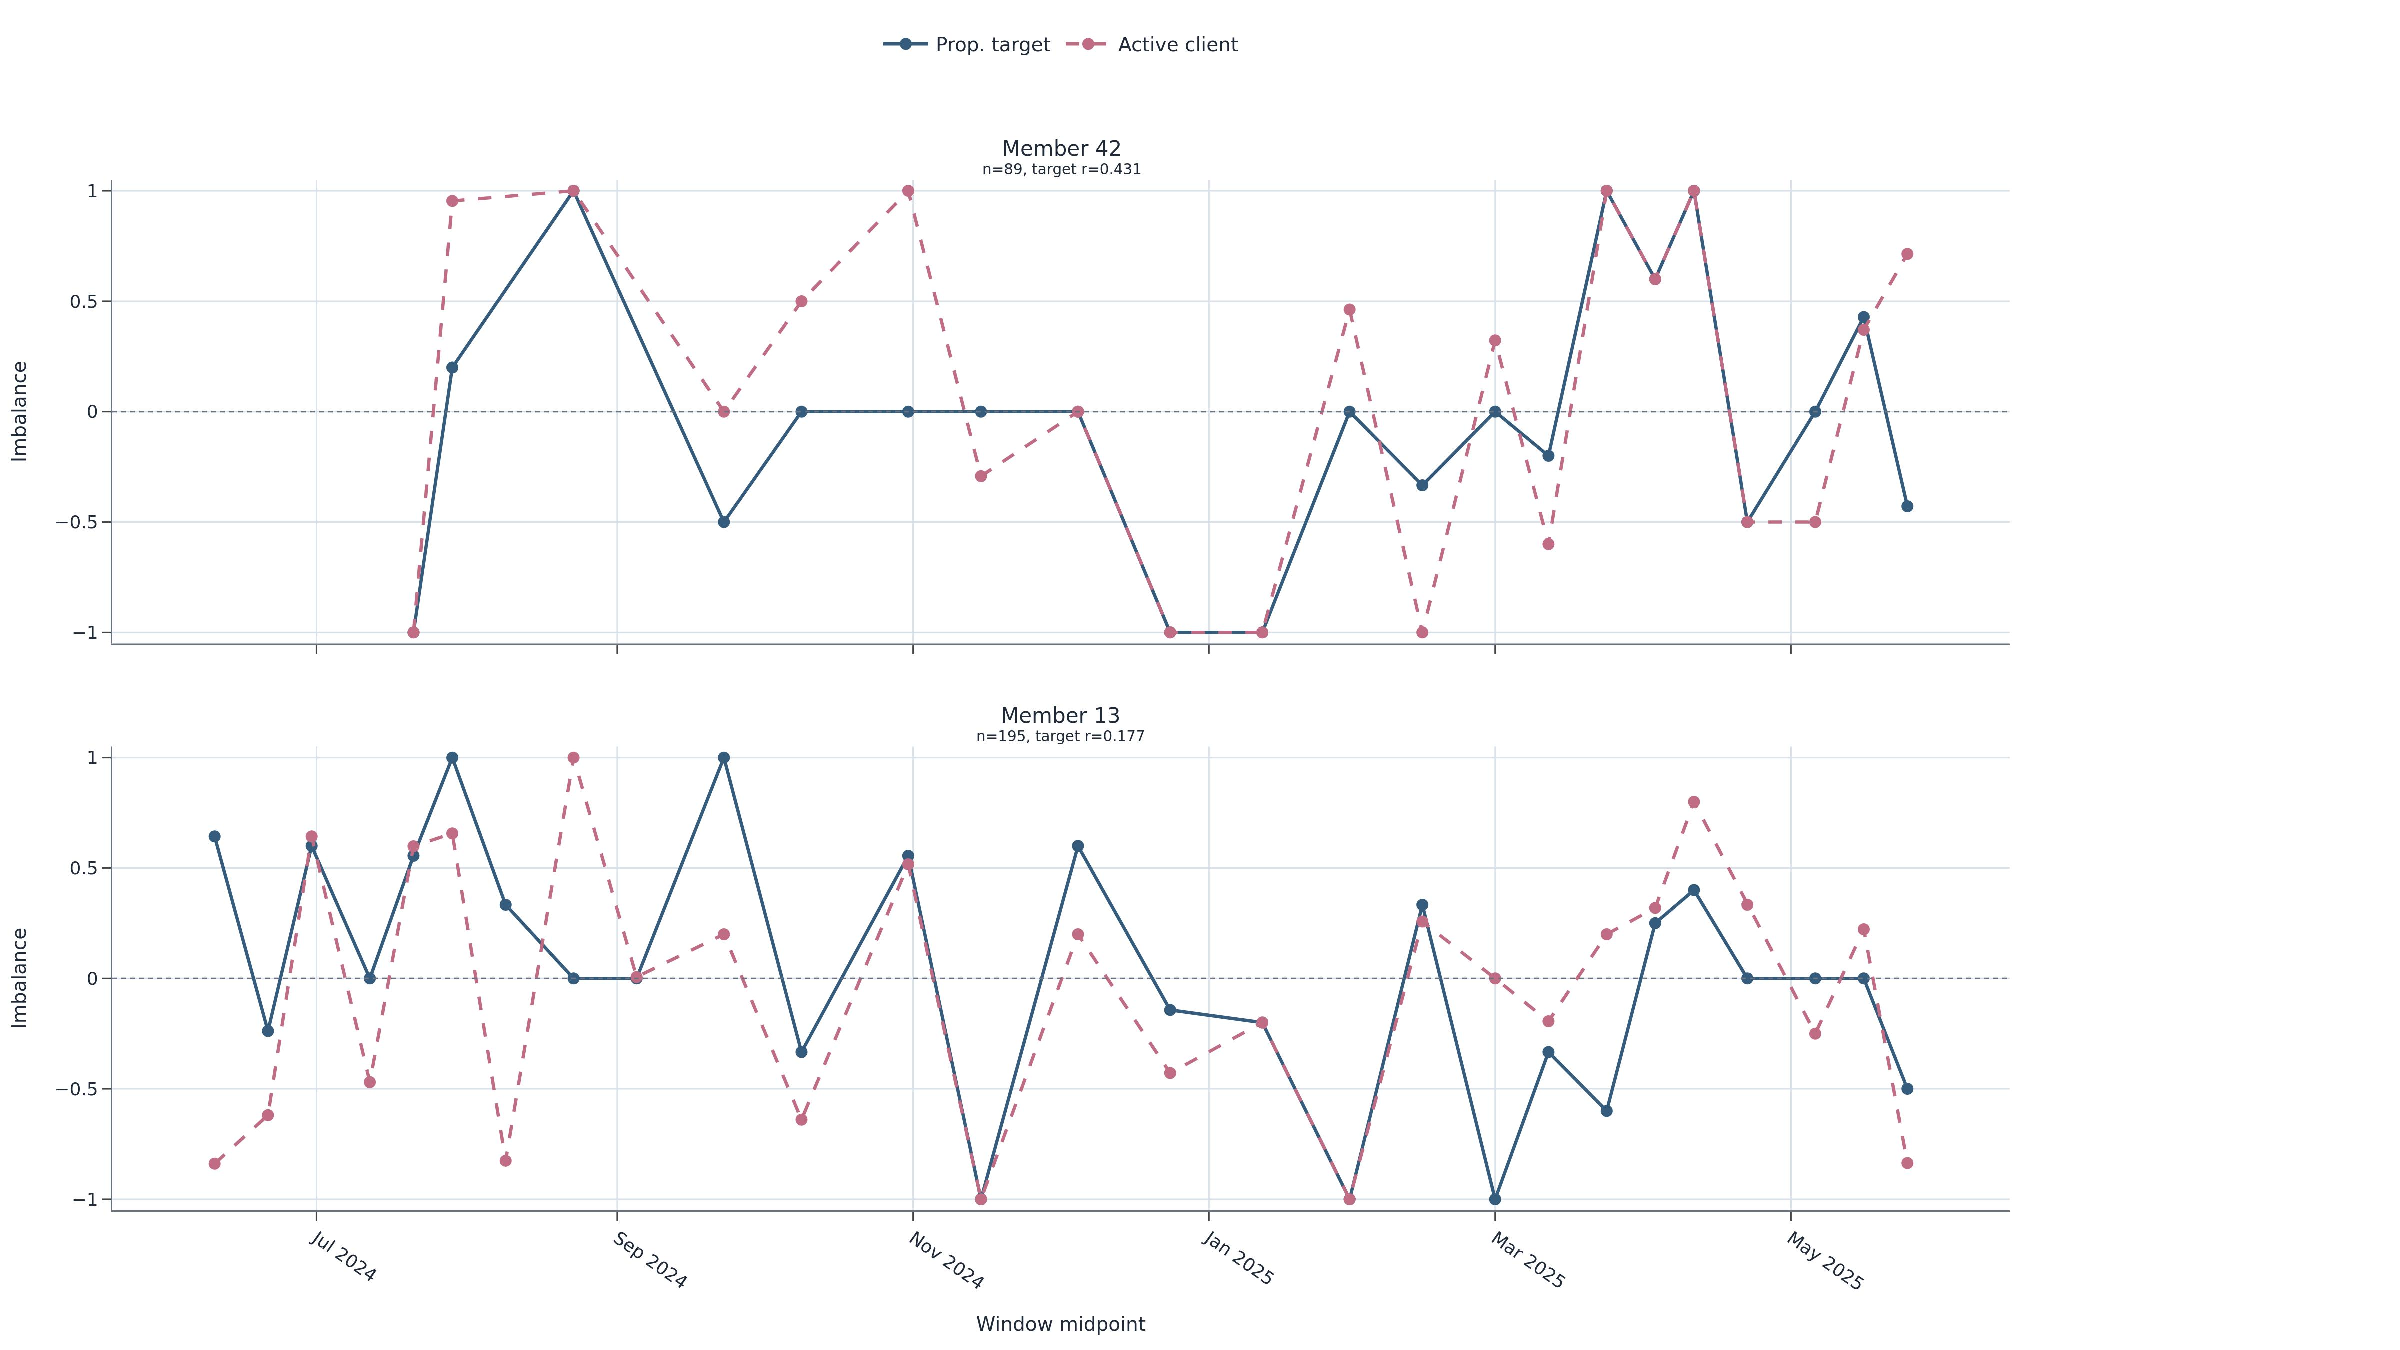
\includegraphics[width=\textwidth]{images/member_active_overlap_crowding/png/member_comovement_same_isin_all_active}
    \caption{Window-level co-movement for the two strongest positive members.}
  \end{subfigure}
  \caption{Active member-level prop--client alignment. The top panel reports
  $r_m^{\mathrm{act}}$ for members with at least 30 valid proprietary targets.
  The bottom panel compares the proprietary target-direction imbalance with the
  active client imbalance for Members 42 and 13 in non-overlapping
  5-trading-day windows.}
  \label{fig:member_active_overlap_crowding}
\end{figure}

Overall, the active-overlap evidence is not one of systematic alignment across
all members. It is instead member-specific. Most members with sufficient local
overlap are close to neutral, while a small number of members, especially
Member 42, exhibit sizeable positive correlations with their own active
client flow. We therefore interpret the analysis as a screening device for
member-level episodes of prop--client alignment. Positive values are consistent
with a front-running concern, but they are not proof of intent: common
information, inventory management, client facilitation, and execution
synchronisation can generate similar co-movement patterns.


\FloatBarrier

\section{Conclusion}
\label{sec:conclusion}

Using trade-by-trade data for FTSE MIB constituents from 2024/06/03 to 2025/05/30, we reconstruct member-level metaorders and
compare proprietary and client aggressive flow within a common framework. The main results are:

\begin{itemize}
  \item Basic properties differ mainly through aggressiveness rather than through radically different distributional
  shapes. Both groups display broad, heavy-tailed distributions for duration, size, relative size, and participation rate, but
  proprietary metaorders are executed with systematically higher participation rates than client metaorders
  (Section~\ref{sec:descriptive_properties}, Table~\ref{tab:distribution-means-medians}).

  \item Price impact is concave for both groups, but the impact law differs sharply by trading capacity. Client flow is
  close to the square-root benchmark, with $\hat\gamma = 0.5082 \pm 0.0228$, whereas proprietary flow is substantially more concave,
  with $\hat\gamma = 0.3662 \pm 0.0083$. In addition, the scale parameter is much larger for client flow
  ($Y_{\mathrm{client}}/Y_{\mathrm{prop}} \approx 1.76$), but this does not imply that the client fit lies
  uniformly above the proprietary one. Because the proprietary exponent is lower, the fitted proprietary curve lies above the
  client curve over most of the observed $\phi$ range and crosses it only around $\phi \approx 1.9 \times 10^{-2}$.
  (Section~\ref{subsec:impact_models}, Figure~\ref{fig:impact_vs_size_pw}).
  
  \item The dynamic response also differs across groups. After execution, proprietary metaorders retain a larger fraction
  of peak impact than client metaorders: at $\tau=3$, $\bar I(\tau{=}3)/\bar I(\tau{=}1)\approx 0.75$ for proprietary flow versus
  $\approx 0.57$ for client flow. This suggests a more persistent component for proprietary impact and a larger transient component
  for client executions (Section~\ref{subsec:impact-paths}, Figure~\ref{fig:normalized_impact_paths}).

  \item Crowding is economically meaningful in both segments, but it is clearly stronger for client flow. Within-group
  direction--imbalance correlations are positive and significant for both proprietary and client metaorders, equal to
  $r=0.108$ (95\% CI $[0.102,0.113]$) and $r=0.187$ (95\% CI $[0.180,0.196]$), respectively. Crowding also strengthens with
  participation rate, especially for clients, while cross-group relations remain weak and slightly contrarian. The all-vs-all
  correlations point in the same direction: client metaorders are more aligned with the aggregate market-side imbalance than
  proprietary metaorders (Section~\ref{sec:crowding}, Figure~\ref{fig:crowding_rolling_timeseries},
  Figure~\ref{fig:crowding_vs_eta_local}, Figure~\ref{fig:crowding_vs_eta_cross}).
  When daily crowding is linked directly to impact, more crowded metaorders do have larger impact, but the premium is larger for
  client flow; in pooled bin-level regressions, crowding enters positively while the proprietary dummy remains large and
  significant. A finer active-overlap analysis shows that proprietary metaorders are not exposed to a larger
  time-weighted count of overlapping metaorders, but their overlapping flow is more directionally aligned. Adding these active-overlap
  controls reduces the proprietary coefficient by about 16\% in metaorder-level regressions. In the log-binned WLS specification,
  which mirrors the original power-law fit, the positive proprietary coefficient becomes smaller and statistically insignificant after
  active-overlap controls enter.
  Thus crowding explains a material part of the proprietary impact premium, especially through directional active overlap, but not
  through a simple count of overlapping metaorders
  (Section~\ref{subsec:crowding_impact}, Tables~\ref{tab:crowding_impact_terciles}--\ref{tab:active_overlap_wls_regression}).

  \item At the executing-member level, prop--client co-movement is small on average but not absent. The mean per-member
  correlation is close to zero, yet the pooled correlation between proprietary direction and the imbalance of the same member's
  client flow is positive and statistically different from zero ($0.011$, 95\% CI $[0.001,0.022]$; permutation $p=0.014$). The
  evidence is episodic and heterogeneous across members rather than uniform over time (Section~\ref{subsec:member_level_crowding},
  Figure~\ref{fig:hist_imbcorr}, Figure~\ref{fig:heatmap_imbcorr}). A more local active-overlap version of the same statistic
  confirms this heterogeneity: the pooled same-ISIN active correlation is small ($0.036$, 95\% CI $[-0.032,0.104]$), but one
  member exhibits a sizeable positive correlation with own active client flow ($r_m^{\mathrm{act}}=0.431$, 95\% CI
  $[0.249,0.614]$). Thus member-level prop--client alignment is not pervasive, but some members display recurrent local
  co-movement with their clients (Section~\ref{subsec:member_active_overlap_crowding},
  Figure~\ref{fig:member_active_overlap_crowding}).
\end{itemize}

Taken together, the results point to a coherent economic picture. Client metaorders are more crowded on the
daily same-ISIN horizon and display a larger unconditional crowding premium, but the static impact ranking depends on the
relative-size range considered: despite the larger client intercept $Y$, the more concave proprietary fit lies above the client
fit over most of the observed $\phi$ range and crosses it only for sufficiently large $\phi$. Client impact also decays more
strongly after execution, whereas proprietary metaorders leave a more persistent footprint in prices. The active-overlap results
suggest that part of this difference is associated with directional overlap during execution; the remaining gap is specification
dependent, shrinking partially in metaorder-level regressions and disappearing in the lower-dimensional binned WLS check. The relevant
heterogeneity is therefore not limited to size or execution speed alone: it also reflects differences in execution motives,
information content, and interaction with the surrounding order-flow environment.

More broadly, the paper shows that proprietary and client metaorders should not be pooled into a single object. Pooling them would
mask differences that matter for empirical impact measurement, for transaction-cost modelling, and for the interpretation of
crowding and intermediation in the market. In this sense, the main contribution of the paper is not only to document distinct
impact curves, but to show that who trades is itself an essential state variable for understanding how large orders move prices.
These results also have a supervisory implication. They do not provide 
evidence of informed trading or misconduct, but they show that trading capacity is an 
economically relevant variable for interpreting price formation. For market surveillance, 
granular transaction data that distinguish proprietary and client activity can therefore 
help assess whether observed price movements are better understood from individual order 
characteristics alone or from the broader execution environment, including contemporaneous 
directional overlap. Trading capacity should consequently be treated not merely as an 
execution label, but as useful context when evaluating the market relevance of trading 
activity.

\newpage 

\appendix

\section{Member-Nationality Diagnostics and Italian-Member Robustness}
\label{app:member_nationality_results}
\label{app:it_member_results}

This appendix collects all results conditioned on the member-nationality label.
The label refers to the executing member (broker), not necessarily to the final
investor, and is therefore used only as a descriptive diagnostic. The main text
conditions on trading capacity---proprietary versus client flow---and reports
aggregate estimates.

\subsection{Nationality composition of executing members}
\label{subsec:metaorder_nationality}

At the member level, we can assign each metaorder to an Italian (IT) or foreign
executing broker using the member nationality mapping. The comparison with overall
trading activity helps clarify the result. In proprietary flow, Italian members are
already marginal in the market as a whole, accounting for only 1.94\% of traded
volume, and they are even less represented in the metaorder sample, with 0.36\% of
metaorders (2,093) and 0.57\% of metaorder volume. Only 11.00\% of Italian proprietary
volume is executed through detected metaorders, compared with 38.09\% for foreign
members. In client flow, the message is different: Italian members are not small
overall, since they account for 52.72\% of traded volume, but they contribute only
9.40\% of client metaorders (24,111) and 9.77\% of client metaorder volume.
Equivalently, only 4.15\% of Italian client volume is executed through detected
metaorders, against 42.69\% for foreign members. Thus, the dominance of foreign
brokers in the metaorder sample is not merely a reflection of larger aggregate
activity; it also reflects a much stronger tendency to execute through metaorder-like
order splitting, especially on the client side. Across both flows combined, Italian
members account for 26.34\% of traded volume but only 3.10\% of detected metaorders.
Aggregate distributions, impact estimates, and crowding results are therefore driven
predominantly by foreign-member execution.

\begin{table}[th!]
  \centering
  \begin{tabular}{lcc}
    \toprule
    Flow & IT & Foreign \\
    \midrule
    Proprietary & 2,093 (0.36\%) & 586,450 (99.64\%) \\
    Client (non-proprietary) & 24,111 (9.40\%) & 232,260 (90.60\%) \\
    \bottomrule
  \end{tabular}
  \caption{Member nationality split at the member level (FTSEMIB sample). Percentages are computed on metaorders with
  known member nationality.}
  \label{tab:metaorder_nationality_share}
\end{table}

Given this extreme skew, the nationality-conditioned results below must be interpreted cautiously, especially for
proprietary IT flow.

\FloatBarrier

\subsection{Italian-member dynamic impact paths}
\label{app:it_member_impact_paths}

As a robustness diagnostic, Figure~\ref{fig:normalized_impact_paths_it} reports the dynamic-impact exercise for the
Italian executing-member subsample. The picture is materially different from the aggregate one: the pooled Italian paths
are much noisier and, in both proprietary and client flow, the mean signed impact path is negative for most of the horizon.
Taken at face value, this means that Italian executing brokers have negative average impact in this subsample, in the sense
that prices move on average against the direction of their metaorders after execution starts. The buy/sell split also does
not recover the clean, stable pattern seen in the full sample, especially for proprietary Italian metaorders, whose
confidence bands are very wide. We therefore read the negative Italian path as a descriptive feature of the sample rather
than as conclusive evidence of a distinct structural regime.

By contrast, the corresponding foreign-member paths are visually indistinguishable from the overall curves in
Figure~\ref{fig:normalized_impact_paths}. This is exactly what one should expect from the composition results in
Section~\ref{subsec:metaorder_nationality}: foreign brokers account for 99.64\% of proprietary metaorders and 90.60\%
of client metaorders, so the aggregate dynamic-impact estimates are effectively foreign-member estimates.

\begin{figure}[t]
  \centering
  \begin{adjustwidth}{0.01\textwidth}{0.01\textwidth}
    \centering
    \begin{subfigure}[t]{0.49\linewidth}
      \centering
      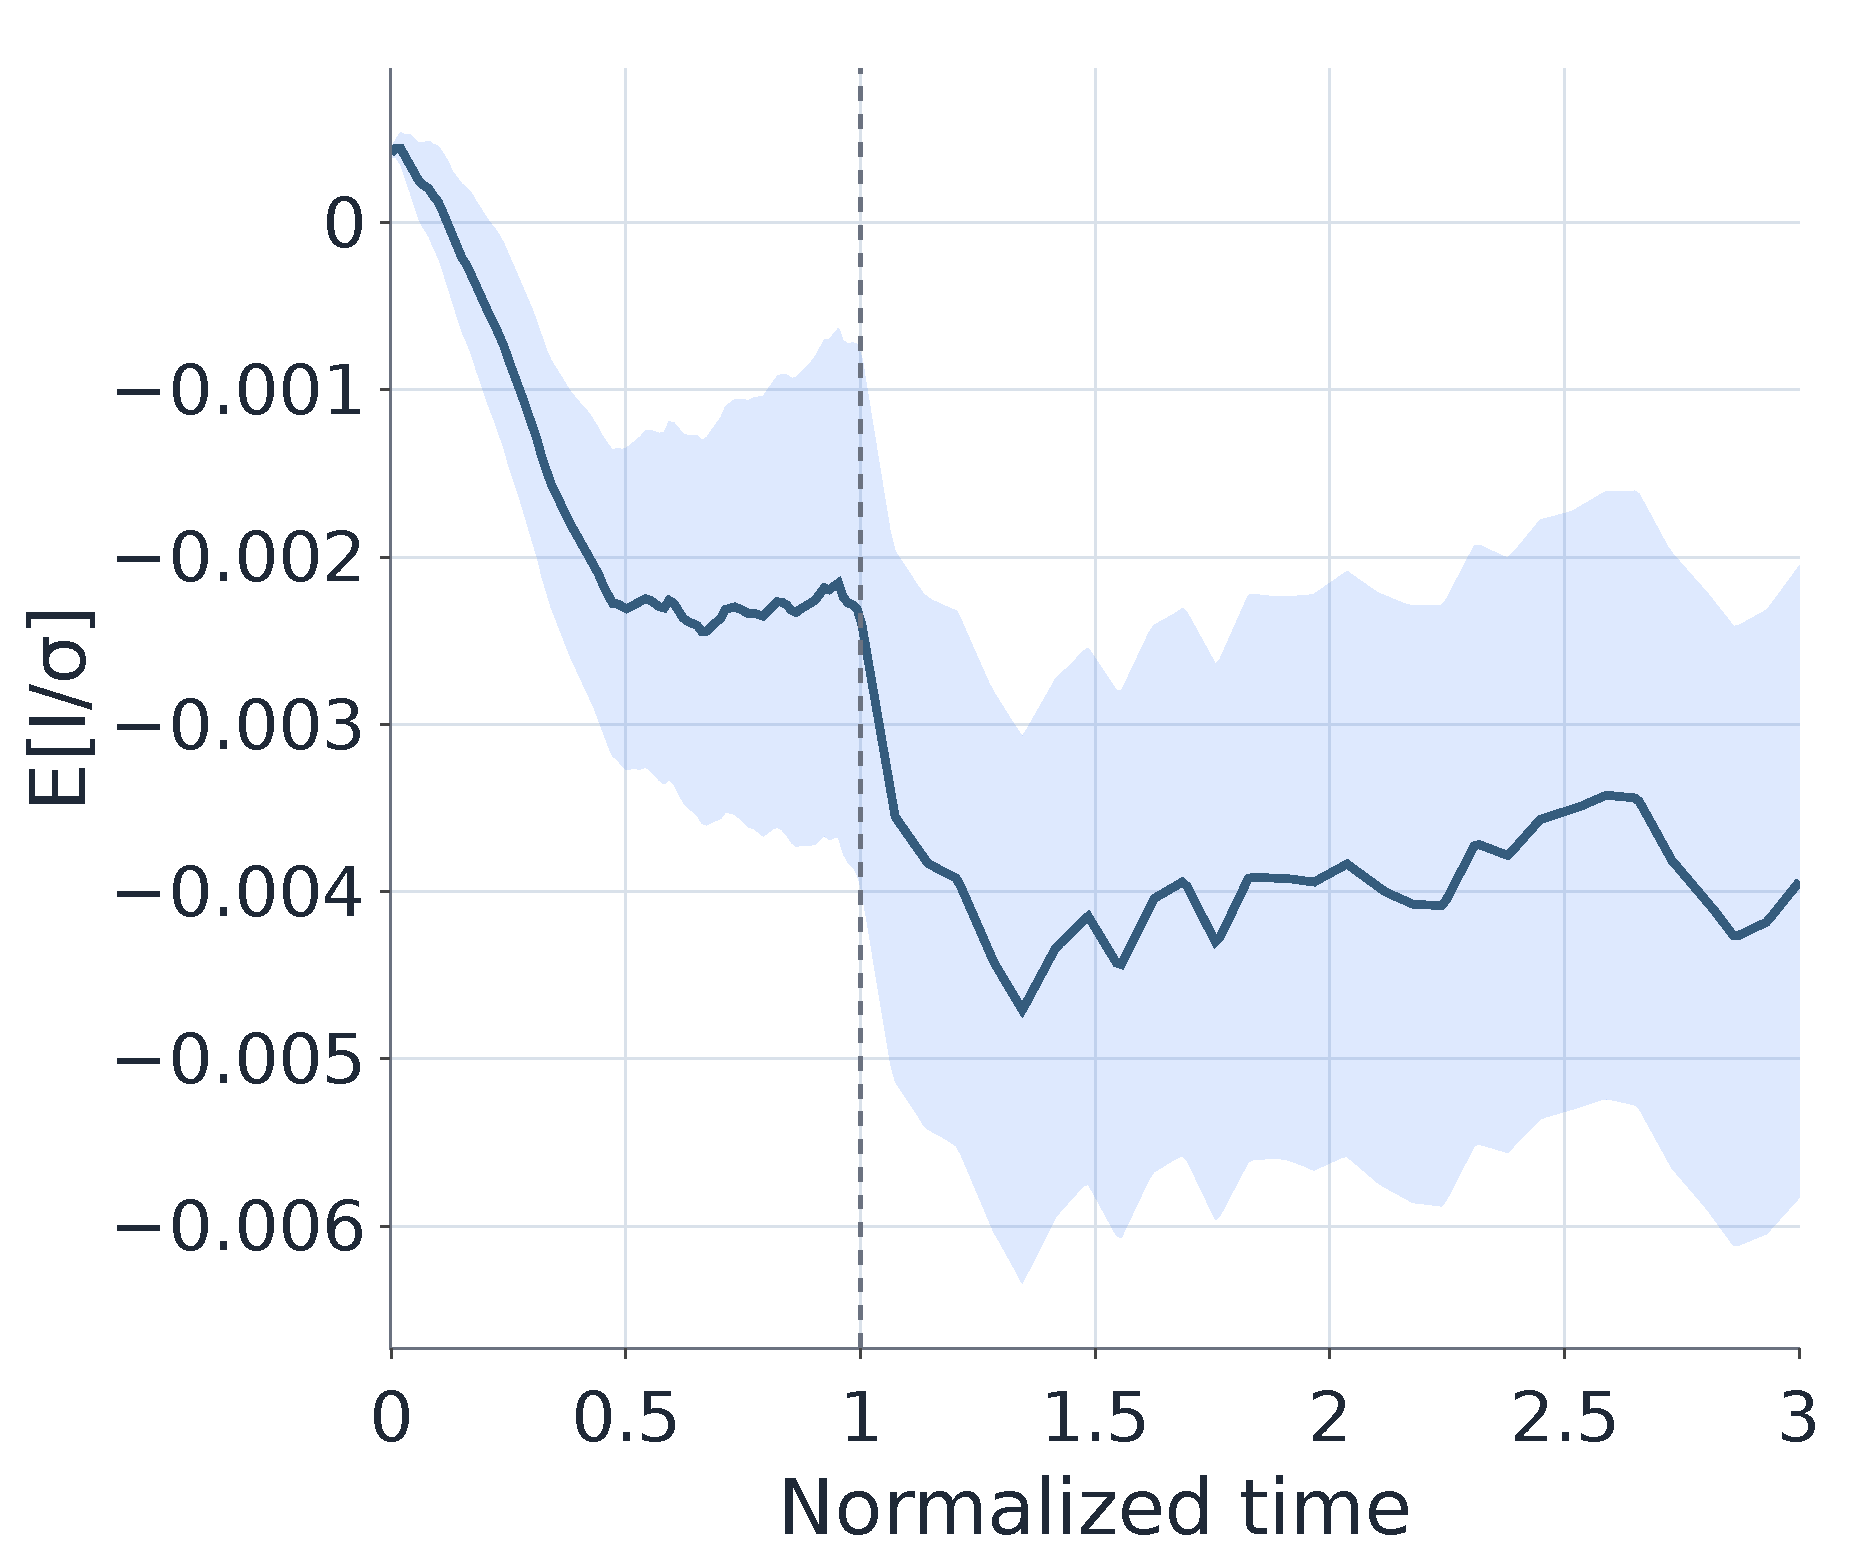
\includegraphics[width=\linewidth]{images/member_proprietary/png/normalized_impact_path_member_proprietary_member_nationality_it}
      \caption{Proprietary: overall}
    \end{subfigure}
    \begin{subfigure}[t]{0.49\linewidth}
      \centering
      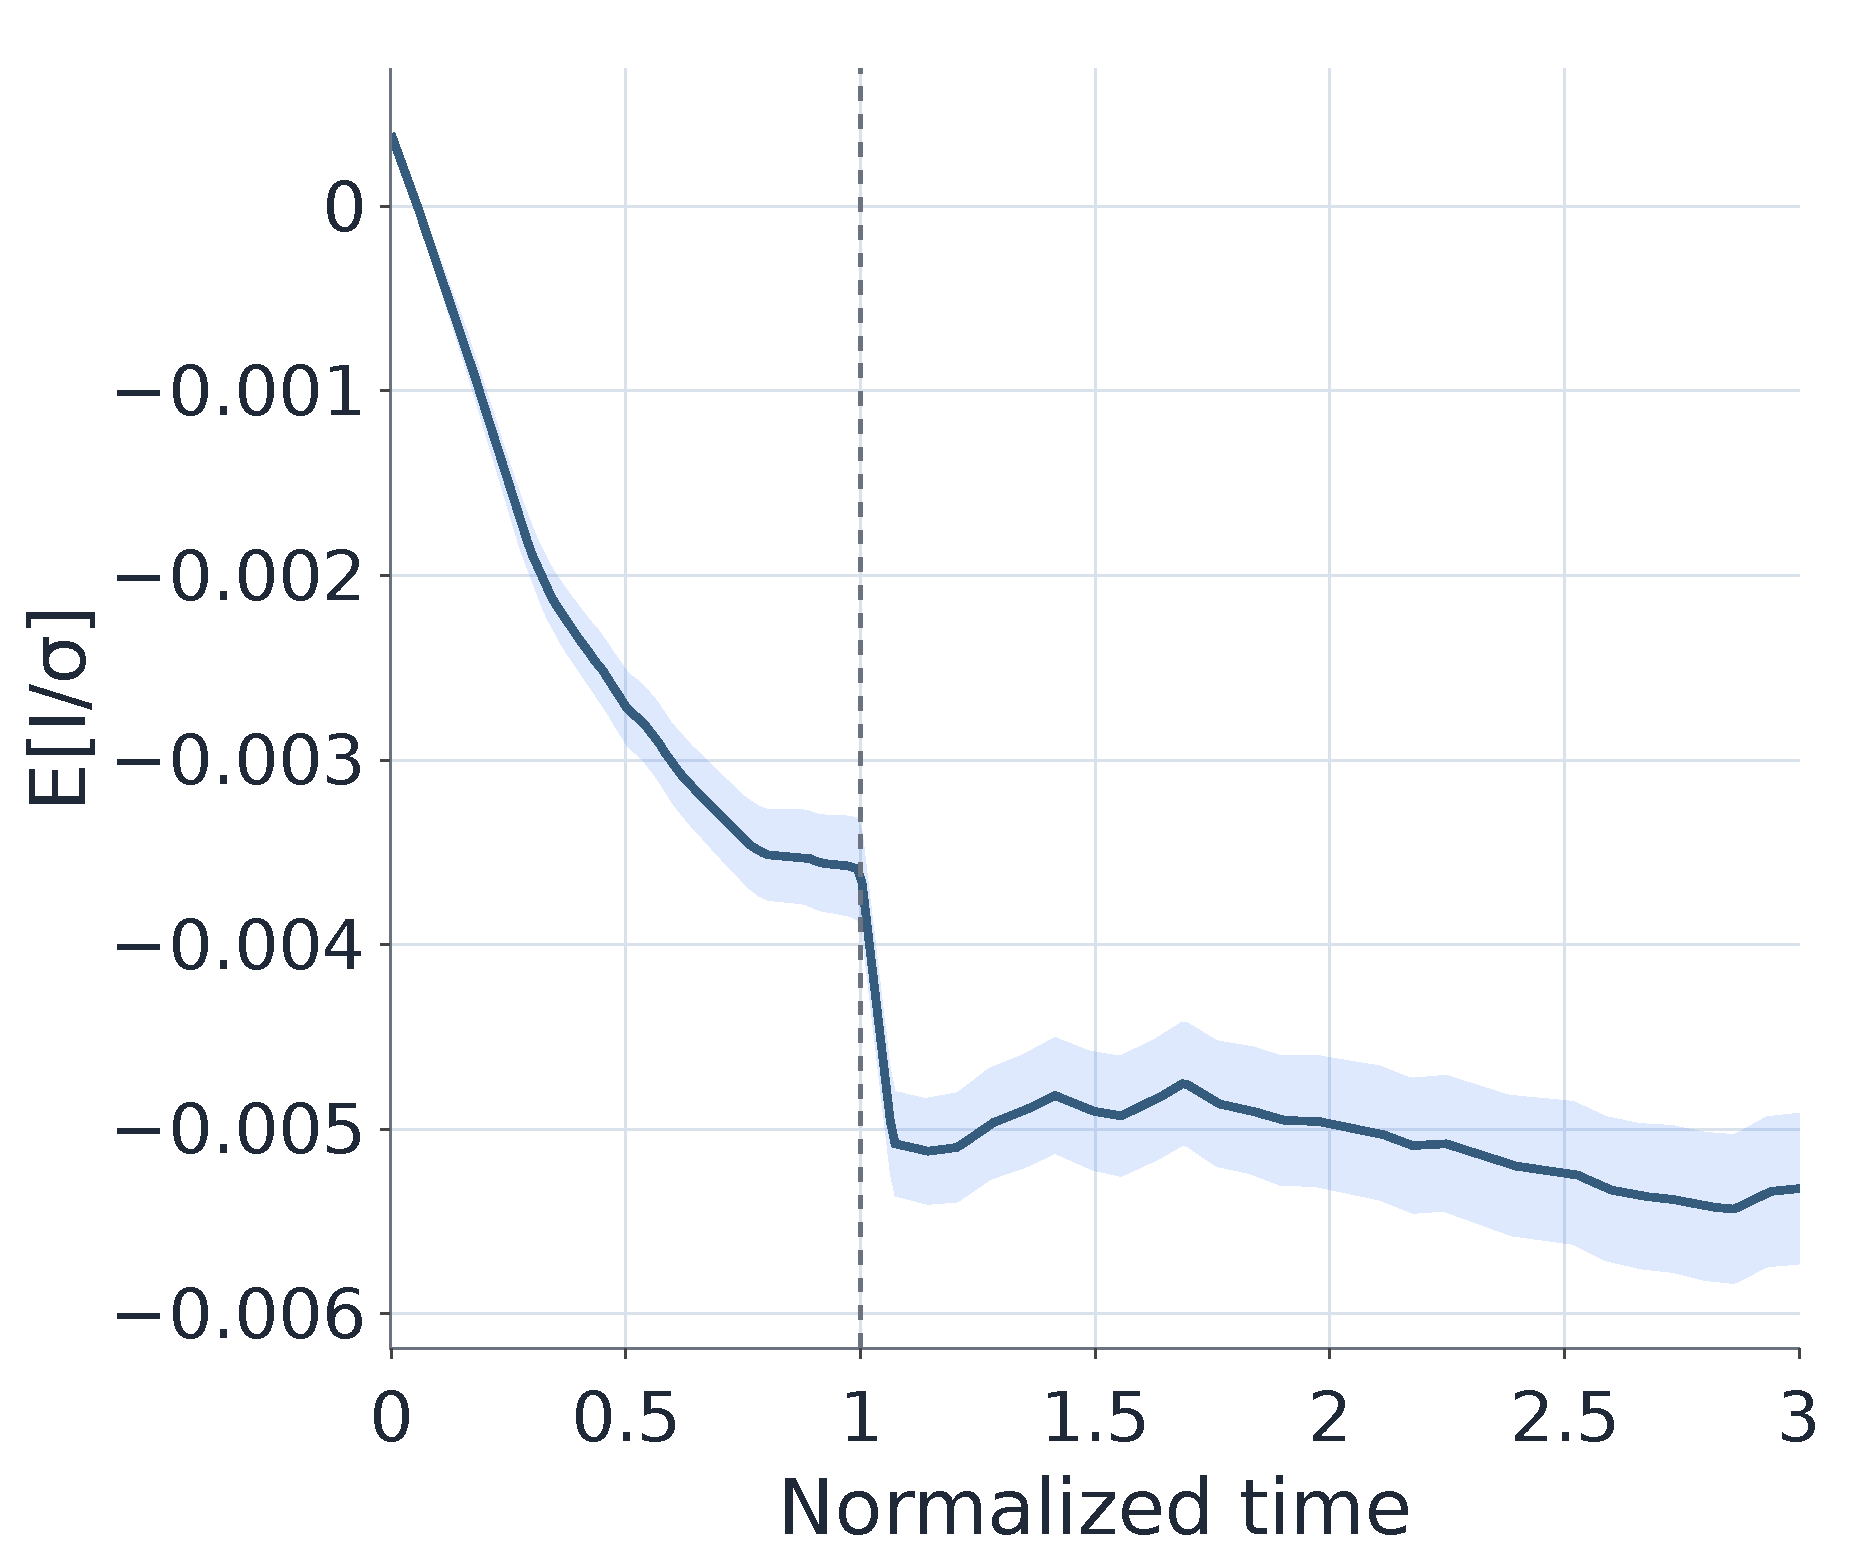
\includegraphics[width=\linewidth]{images/member_non_proprietary/png/normalized_impact_path_member_non_proprietary_member_nationality_it}
      \caption{Client: overall}
    \end{subfigure}
  \end{adjustwidth}
  \caption{Mean normalised impact paths $\bar I_G(\tau)$ for the Italian executing-member subsample. The analogous
  foreign-member paths are omitted because they are visually indistinguishable from the overall curves. Time is
  normalised so that $\tau = 0$ at the start of the metaorder and $\tau = 1$ at its end; the dashed line marks
  $\tau = 1$. Shaded regions are $\pm$SEM.}
  \label{fig:normalized_impact_paths_it}
\end{figure}

\FloatBarrier

\subsection{Italian-member summary statistics}
\label{app:it_member_summary_statistics}
This subsection reports summary statistics for the subsample of member-level metaorders executed by Italian members
(member nationality tag = IT). As discussed in Section~\ref{subsec:metaorder_nationality}, the proprietary IT
subsample is small, so estimates should be interpreted cautiously.
% AUTO-GENERATED FILE. DO NOT EDIT BY HAND.
% Generated by: scripts/export_paper_appendix_it.py
% Generated on: 2026-02-23T15:22:38
% Source summary CSV: out_files/ftsemib/paper_appendix/appendix_it_metaorder_stats_summary.csv

\begin{table}[t]
  \centering
  \small
  \begin{tabular}{lcc}
    \toprule
    Quantity & Proprietary (IT) & Client (IT) \\
    \midrule
    Metaorders (N) & 2093 & 24111 \\
    Buys / sells & 1033 / 1060 & 13607 / 10504 \\
    Duration $T$ (min): mean / median / IQR & 52.74 / 42.44 / 58.84 & 39.44 / 25.16 / 45.35 \\
    Inter-arrival $\Delta t$ (min): mean / median / IQR & 4.87 / 0.39 / 3.77 (N=22676) & 4.49 / 1.15 / 4.37 (N=211746) \\
    Volume $Q$ (shares): mean / median / IQR & 49221 / 10950 / 25409 & 40465 / 8131 / 18792 \\
    Relative size $Q/V$: mean / median / IQR & 0.0048 / 0.0014 / 0.0046 & 0.0030 / 0.0011 / 0.0022 \\
    Participation rate $\eta$: mean / median / IQR & 0.0679 / 0.0185 / 0.0726 & 0.0635 / 0.0191 / 0.0650 \\
    \bottomrule
  \end{tabular}
  \caption{Summary statistics for member-level metaorders executed by Italian members (member nationality tag = IT). Values are mean / median / interquartile range (IQR). Inter-arrival times are computed across child-trade gaps (sample size N is the number of gaps).}
  \label{tab:appendix_it_metaorder_stats}
\end{table}


\FloatBarrier

\begin{thebibliography}{99}

\bibitem{ChakrabartyCoxUpson2024RetailOrderFlow}
B.~Chakrabarty, J.~Cox, and J.~E. Upson.
\newblock The information content of retail order flow: Evidence from fragmented markets.
\newblock \emph{Journal of Banking \& Finance} \textbf{167}, 107275, 2024.
\newblock doi: \href{https://doi.org/10.1016/j.jbankfin.2024.107275}{10.1016/j.jbankfin.2024.107275}.


\bibitem{BacryEtAl2014}
E.~Bacry, A.~Iuga, M.~Lasnier, and C.-A. Lehalle.
\newblock Market impacts and the life cycle of investors orders.
\newblock arXiv preprint arXiv:1412.0217, 2014.

\bibitem{Torre1997}
N.~Torre.
\newblock {BARRA} market impact model handbook.
\newblock BARRA Inc., Berkeley, 1997.

\bibitem{AlmgrenEtAl2005}
R.~Almgren, C.~Thum, E.~Hauptmann, and H.~Li.
\newblock Direct estimation of equity market impact.
\newblock \emph{Risk} \textbf{18}(7), 58--62, 2005.

\bibitem{EngleEtAl2008}
R.~F. Engle, R.~Ferstenberg, and J.~Russell.
\newblock Measuring and modeling execution cost and risk.
\newblock Chicago GSB Research Paper No.~08-09, 2008.

\bibitem{MastromatteoEtAl2014}
I.~Mastromatteo, B.~T{'o}th, and J.-P. Bouchaud.
\newblock Agent-based models for latent liquidity and concave price impact.
\newblock \emph{Physical Review E} \textbf{89}(4), 042805, 2014.

\bibitem{BrokmannEtAl2014}
X.~Brokmann, E.~Serie, J.~Kockelkoren, and J.-P. Bouchaud.
\newblock Slow decay of impact in equity markets.
\newblock arXiv preprint arXiv:1407.3390, 2014.

\bibitem{SatoKanazawa2024}
Y.~Sato and K.~Kanazawa.
\newblock Does the square-root price impact law belong to the strict universal scalings? Quantitative support by a complete survey of the Tokyo Stock Exchange market.
\newblock arXiv preprint arXiv:2411.13965, 2024.

\bibitem{PuckettYan2008}
A.~Puckett and X.~Yan.
\newblock Short-term institutional herding and its impact on stock prices.
\newblock \emph{SSRN Electronic Journal}, 2008.
\newblock doi: \href{https://doi.org/10.2139/ssrn.972254}{10.2139/ssrn.972254}.

\bibitem{Sias2004}
R.~W. Sias.
\newblock Institutional herding.
\newblock \emph{Review of Financial Studies} \textbf{17}(1), 165--206, 2004.
\newblock doi: \href{https://doi.org/10.1093/rfs/hhg035}{10.1093/rfs/hhg035}.

\bibitem{DasguptaPratVerardo2011}
A.~Dasgupta, A.~Prat, and M.~Verardo.
\newblock The price impact of institutional herding.
\newblock \emph{Review of Financial Studies} \textbf{24}(3), 892--925, 2011.
\newblock doi: \href{https://doi.org/10.1093/rfs/hhq137}{10.1093/rfs/hhq137}.

\bibitem{BucciEtAl2020}
F.~Bucci, I.~Mastromatteo, Z.~Eisler, F.~Lillo, J.-P. Bouchaud, and C.-A. Lehalle.
\newblock Co-impact: crowding effects in institutional trading activity.
\newblock \emph{Quantitative Finance} \textbf{20}(2), 193--205, 2020.

\bibitem{BriereEtAl2019}
M.~Briere, C.-A. Lehalle, T.~Nefedova, and A.~Raboun.
\newblock Modelling transaction costs when trades may be crowded: a Bayesian network using partially observable orders imbalance.
\newblock Book chapter, 2019.

\bibitem{zarinelli}
E.~Zarinelli, M.~Treccani, J.~D. Farmer, and F.~Lillo.
\newblock Beyond the square root: Evidence for logarithmic dependence of market impact on size and participation rate.
\newblock \emph{Market Microstructure and Liquidity} \textbf{1}(2), 1550004, 2015.

\bibitem{BucciEtAl2018}
F.~Bucci, M.~Benzaquen, F.~Lillo, and J.-P. Bouchaud.
\newblock Slow decay of impact in equity markets: Insights from the ANcerno database.
\newblock \emph{Market Microstructure and Liquidity} \textbf{4}(3--4), 1950006, 2018.

\bibitem{BucciEtAl2020Invariants}
F.~Bucci, F.~Lillo, J.-P. Bouchaud, and M.~Benzaquen.
\newblock Are trading invariants really invariant? Trading costs matter.
\newblock \emph{Quantitative Finance} \textbf{20}(7), 1059--1068, 2020.

\bibitem{MoroEtAl2009}
E.~Moro, J.~Vicente, L.~G. Moyano, A.~Gerig, J.~D. Farmer, G.~Vaglica, F.~Lillo, and R.~N. Mantegna.
\newblock Market impact and trading profile of hidden orders in stock markets.
\newblock \emph{Physical Review E} \textbf{80}(6), 066102, 2009.

\bibitem{VaglicaEtAl2010}
G.~Vaglica, F.~Lillo, and R.~N. Mantegna.
\newblock Statistical identification with hidden {Markov} models of large order splitting strategies in an equity market.
\newblock \emph{New Journal of Physics} \textbf{12}(7), 075031, 2010.

\bibitem{GomesWaelbroeck2015}
C.~Gomes and H.~Waelbroeck.
\newblock Is market impact a measure of the information value of trades? Market response to liquidity vs. informed metaorders.
\newblock \emph{Quantitative Finance} \textbf{15}(5), 773--793, 2015.

\bibitem{Tsaknaki2025}
I.~Y. Tsaknaki, F.~Lillo, and P.~Mazzarisi.
\newblock Online learning of order flow and market impact with Bayesian change-point detection methods.
\newblock \emph{Quantitative Finance} \textbf{25}(2), 307--322, 2025.

\bibitem{MaitrierEtAl2025}
G.~Maitrier, G.~Loeper, and J.-P. Bouchaud.
\newblock Generating realistic metaorders from public data.
\newblock arXiv preprint arXiv:2503.18199, 2025.

\bibitem{BarndorffNielsen2008}
O.~E. Barndorff-Nielsen, P.~R. Hansen, A.~Lunde, and N.~Shephard.
\newblock Designing realized kernels to measure the ex post variation of equity prices in the presence of noise.
\newblock \emph{Econometrica} \textbf{76}(6), 1481--1536, 2008.

\bibitem{Clauset_2009}
A.~Clauset, C.~R. Shalizi, and M.~E.~J. Newman.
\newblock Power-law distributions in empirical data.
\newblock \emph{SIAM Review} \textbf{51}(4), 661--703, 2009.
\newblock doi: \href{https://doi.org/10.1137/070710111}{10.1137/070710111}.

\bibitem{BouchaudFarmerLillo2008}
J.-P. Bouchaud, J.~D. Farmer, and F.~Lillo.
\newblock How markets slowly digest changes in supply and demand.
\newblock In T.~Hens and K.~R. Schenk-Hopp{'e}, editors, \emph{Handbook of Financial Markets: Dynamics and Evolution}.
\newblock Academic Press, 2008.

% The following references do not appear to be cited in the current text.

% \bibitem{Lou2012}
% D.~Lou.
% \newblock A flow-based explanation for return predictability.
% \newblock \emph{Review of Financial Studies} \textbf{25}(12), 3457--3489, 2012.
% \newblock doi: \href{https://doi.org/10.1093/rfs/hhs103}{10.1093/rfs/hhs103}.

% \bibitem{NaviglioEtAl2025}
% M.~Naviglio, G.~Bormetti, F.~Campigli, G.~Rodikov, and F.~Lillo.
% \newblock Why is the estimation of metaorder impact with public market data so challenging?
% \newblock arXiv preprint arXiv:2501.17096, 2025.

% \bibitem{Guillaume2025}
% G.~Guillaume.
% \newblock The hidden complexity of price formation.
% \newblock PhD thesis, 2025.

% \bibitem{repo}
% D.~M. Di~Nosse.
% \newblock Metaorders_PriceImpact: Study of metaorder price impact using proprietary CONSOB data.
% \newblock GitHub repository, 2025.
% \newblock Available at \url{https://github.com/DanieleMDiNosse/Metaorders_PriceImpact}.



\end{thebibliography}

\end{document}
